\documentclass{scrartcl}
\usepackage{pgfplots}
\usepackage[scaled=0.85]{beramono}
\usepackage{makecell}
\usepackage{multirow} % For merged cells
\usepackage{booktabs} % For better table formatting
\usepackage{calc}
\usepackage{Style_File}
\usepackage{fancyhdr}
\usepackage{tensor}
\usepackage{array}
\usepackage{lmodern}
\everymath{\mathrm{\xdef\tmp{\fam\the\fam\relax}\aftergroup\tmp}}
\definecolor{violet}{rgb}{0.5,0.27,0.45}

\newcolumntype{P}[1]{>{\centering\arraybackslash}p{#1}}
% Recommended preamble:
\usetikzlibrary{arrows.meta}
\usetikzlibrary{backgrounds}
\usepgfplotslibrary{patchplots}
\usepgfplotslibrary{fillbetween}
\pgfplotsset{%
    layers/standard/.define layer set={%
        background,axis background,axis grid,axis ticks,axis lines,axis tick labels,pre main,main,axis descriptions,axis foreground%
    }{
        grid style={/pgfplots/on layer=axis grid},%
        tick style={/pgfplots/on layer=axis ticks},%
        axis line style={/pgfplots/on layer=axis lines},%
        label style={/pgfplots/on layer=axis descriptions},%
        legend style={/pgfplots/on layer=axis descriptions},%
        title style={/pgfplots/on layer=axis descriptions},%
        colorbar style={/pgfplots/on layer=axis descriptions},%
        ticklabel style={/pgfplots/on layer=axis tick labels},%
        axis background@ style={/pgfplots/on layer=axis background},%
        3d box foreground style={/pgfplots/on layer=axis foreground},%
    },
}
\newcommand{\amstitle}[1]{%
  {\Large\MakeUppercase{#1}}% First letter large, rest small caps (simplified)
  % OR for true small caps:
  % {\Large\MakeUppercase{\expandafter\@firstofone#1}\scshape\MakeLowercase{#1}}%
}
\usepackage[left = 1in,
right = 1in,
bottom = 1in,
top = 1in,
a4paper]{geometry}

% \setlength{\headheight}{0.75in}
% \setlength{\oddsidemargin}{0in}
%         \setlength{\evensidemargin}{0in}
%         \setlength{\textwidth}{6.5in}
%         \setlength{\headwidth}{7.3in}
%         \setlength{\textheight}{8.75in}
%         \rfoot{\thepage}
%         \renewcommand{\headrulewidth}{0pt} % Remove the header line
%         \renewcommand{\footrulewidth}{0pt}
\fancyhead[L,C]{}
\fancyhead[R]{PH3203}
\usepackage[hidelinks]{hyperref}
\hypersetup{colorlinks=true,linkcolor=cyan!80!black, citecolor=YellowOrange,urlcolor=cyan!80!black}
\fancyhead[L]{ Entanglement Classification using Knots}
\fancyfoot[C]{\thepage}
\fancyfoot[R,L]{}
\usetikzlibrary{calc}
\pagestyle{fancy}
\renewcommand{\headrulewidth}{0.4pt}
\definecolor{titleblue}{RGB}{0, 80, 120}
\usepackage{longtable} 


\begin{document}
\makeatletter
\begin{titlepage}
    \begin{tikzpicture}[remember picture, overlay]
        \draw[black!80!blue, line width=2pt] 
            ($(current page.north west)+(0.6cm,-0.6cm)$) rectangle 
            ($(current page.south east)+(-0.6cm,0.6cm)$);
    \end{tikzpicture}
    \vspace*{2cm}
    %\begin{center}
        %{\sffamily\bfseries
        %\Huge\textbf{\textcolor{blue!30!black}{\texttt{Classification of Entanglement using Knots}}}\\[0.7cm]
        %\LARGE \textcolor{black!50!cyan}{\texttt{A Topological Approach to Quantum States}}\\[1.0cm]
        %\Large PH3203 Term Project Report \\[0.2cm]
        %\Large \textit{Instructor: Prof. Sourin Das}}\\[1.5cm]\end{center}

        \begin{center}
            {\rmfamily
                \Huge{\textcolor{blue!30!black}{%
                    \textmd{\HUGE{{C}}}{LASSIFICATION {\HUGE{O}}F \\[0.3cm]{\HUGE E}NTANGLEMENT {\HUGE U}SING {\HUGE K}NOTS}%
                }}\\[0.7cm]
                
                \LARGE \textcolor{black!50!cyan}{%
                    \texttt{A \textsc{Topological Approach to Quantum States}}%
                }\\[1.0cm]
                
                \Large \textsc{PH3203 Term Project Report} \\[0.2cm]
                \Large \textit{Instructor: Prof. Sourin Das}%
            }\\[1.5cm]
            \end{center}
       
        \begin{figure}[H]
            \centering
            \includesvg[scale=0.4]{pics/Square_knot.svg}
        \end{figure}
        \vspace{1cm}
        \begin{table}[H]
			\centering
			\def\arraystretch{2}\tabcolsep=1.2cm
			\begin{tabular}{cc}
				\thead{\Large \texttt{\textbf{{\LARGE  S}agnik {\LARGE S}eth }}                      \\[5pt] \large 22MS026} &
				\thead{\Large  \texttt{\textbf{{\LARGE J}essica {\LARGE D}as} }              \\[5pt] \large 22MS157} \\
				\multicolumn{2}{c}{\thead{\Large  \texttt{\textbf{{\LARGE S}ayan {\LARGE K}armakar}} \\[5pt] \large 22MS163}}
			\end{tabular}
		\end{table}
        \vspace{0.5cm}
       \begin{center}
       \textbf{ Depart of Physical Sciences}\\
        \textbf{IISER Kolkata}
        \begin{figure}[H]
            \centering
            \includesvg[scale=0.2]{pics/IISER-Kolkata-logo-vector-01.svg}
        \end{figure}
       \end{center}
\end{titlepage}

  
       
\tableofcontents
\newpage
\section{Introduction}
%     Source - Wikipedia

Classifying entanglement is essential because not all quantum states are equally useful for quantum information tasks. Different types of entanglement serve as distinct resources, each suited to specific applications such as quantum algorithms or secure communication protocols like quantum key distribution. Understanding and identifying these entanglement types helps determine how quantum states can be used and manipulated effectively. hi hi hi this is testing\\[0.3cm]
SLOCC (Stochastic Local Operations and Classical Communication) is a method for classifying quantum entanglement. It defines equivalence classes of quantum states based on whether they can be converted into each other using local operations (on individual qubits) and classical communication.\\[0.3cm]
This idea has been used successfully to study three-qubit states, classifying four-qubit states Methods have been developed for handling systems with even more qubits [7,8].[0.3cm]
In this paper, the authors have proposed an alternative classification scheme for quantum entanglement based on topological links.\\[0.3cm]
One of the first images that comes to mind when we think of entanglement is that of entangled threads. Naturally, one wonders if we could study quantum entanglement using entangled 'knots'. Aravind~\cite{Aravind1997} was the first to point out the connections between entangled quantum states and classical knot configurations, focussing on similarity between 3-particle GHZ state and Borromean rings. He associated each particle with a ring, entanglement of any set of particles as inability to separate their corresponding rings, and measurement of particle state as cutting its ring. But he noted that performing the measurement in different basis would not lead to the same conclusions. This limit in analogy was dealt with by Sugita~\cite{Sugita2007-ko}. He proposed that cutting the ring is equivalent to tracing out the corresponding particle from the density operator, which is a basis-independent operation. This represents viewing the system as though that particle is no longer present. Moreover, the trace operation helps to generalise the idea to quantum systems with more than 2 levels.  

\section{How it all began$\ldots$}
In his 1997 paper, Aravind points out the connection between three-particle GHZ (Greenberger–Horne–Zeilinger)
state and Borromean Rings. The latter is a set of three interlinked rings that can not be pulled apart. However, if one of the rings is cut, the other two are separated. The GHZ state of 3 spin-$\frac{1}{2}$ particles has the form:

\[
\ket{\Psi} = \frac{1}{\sqrt{2}} (\ket{0}_1\ket{0}_2\ket{0}_3 - \ket{1}_1\ket{1}_2\ket{1}_3)
\]
where $\ket{0}$ and $\ket{1}$ are eigenvectors of the operator $\hat{S}_z$
\[
\hat{S}_z\ket{0} = \frac{\hbar}{2}\ket{0}\qquad
\hat{S}_z\ket{1} = -\frac{\hbar}{2}\ket{1}
\]
\begin{figure}[H]
    \centering
   \scalebox{0.8}{ 

\tikzset{every picture/.style={line width=0.75pt}} %set default line width to 0.75pt        

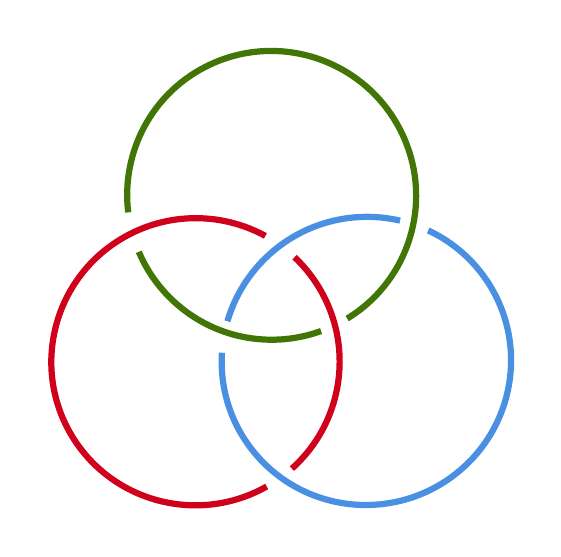
\begin{tikzpicture}[x=0.75pt,y=0.75pt,yscale=-1,xscale=1]
%uncomment if require: \path (0,300); %set diagram left start at 0, and has height of 300

%Shape: Arc [id:dp49278097545949884] 
\draw  [draw opacity=0][line width=2.25]  (328.62,163.73) .. controls (321.19,166.44) and (313.18,167.92) .. (304.82,167.92) .. controls (276.06,167.92) and (251.39,150.46) .. (240.8,125.56) -- (304.82,98.33) -- cycle ; \draw  [color={rgb, 255:red, 65; green, 117; blue, 5 }  ,draw opacity=1 ][line width=2.25]  (328.62,163.73) .. controls (321.19,166.44) and (313.18,167.92) .. (304.82,167.92) .. controls (276.06,167.92) and (251.39,150.46) .. (240.8,125.56) ;  
%Shape: Arc [id:dp7313937278600963] 
\draw  [draw opacity=0][line width=2.25]  (380.22,115.26) .. controls (389.75,119.69) and (398.4,126.36) .. (405.34,135.15) .. controls (429.07,165.23) and (423.73,208.87) .. (393.41,232.62) .. controls (363.09,256.37) and (319.27,251.24) .. (295.54,221.15) .. controls (284.6,207.29) and (279.84,190.54) .. (280.85,174.18) -- (350.44,178.15) -- cycle ; \draw  [color={rgb, 255:red, 74; green, 144; blue, 226 }  ,draw opacity=1 ][line width=2.25]  (380.22,115.26) .. controls (389.75,119.69) and (398.4,126.36) .. (405.34,135.15) .. controls (429.07,165.23) and (423.73,208.87) .. (393.41,232.62) .. controls (363.09,256.37) and (319.27,251.24) .. (295.54,221.15) .. controls (284.6,207.29) and (279.84,190.54) .. (280.85,174.18) ;  
%Shape: Arc [id:dp9082888658781946] 
\draw  [draw opacity=0][line width=2.25]  (235.71,106.58) .. controls (232.15,77.58) and (247.26,48.37) .. (275.16,35.34) .. controls (309.93,19.08) and (351.4,34.11) .. (367.78,68.91) .. controls (383.06,101.37) and (371.11,139.56) .. (341.2,157.73) -- (304.82,98.33) -- cycle ; \draw  [color={rgb, 255:red, 65; green, 117; blue, 5 }  ,draw opacity=1 ][line width=2.25]  (235.71,106.58) .. controls (232.15,77.58) and (247.26,48.37) .. (275.16,35.34) .. controls (309.93,19.08) and (351.4,34.11) .. (367.78,68.91) .. controls (383.06,101.37) and (371.11,139.56) .. (341.2,157.73) ;  
%Shape: Arc [id:dp7357603003827937] 
\draw  [draw opacity=0][line width=2.25]  (302.44,238.64) .. controls (269.08,257.52) and (226.71,245.99) .. (207.75,212.86) .. controls (188.77,179.69) and (200.44,137.44) .. (233.81,118.48) .. controls (255.62,106.09) and (281.32,106.72) .. (301.8,117.92) -- (268.17,178.53) -- cycle ; \draw  [color={rgb, 255:red, 208; green, 2; blue, 27 }  ,draw opacity=1 ][line width=2.25]  (302.44,238.64) .. controls (269.08,257.52) and (226.71,245.99) .. (207.75,212.86) .. controls (188.77,179.69) and (200.44,137.44) .. (233.81,118.48) .. controls (255.62,106.09) and (281.32,106.72) .. (301.8,117.92) ;  
%Shape: Arc [id:dp02993817280793909] 
\draw  [draw opacity=0][line width=2.25]  (283.51,159.01) .. controls (286.66,148.19) and (292.5,137.97) .. (301.03,129.39) .. controls (318.8,111.52) and (343.85,105.22) .. (366.69,110.55) -- (350.44,178.15) -- cycle ; \draw  [color={rgb, 255:red, 74; green, 144; blue, 226 }  ,draw opacity=1 ][line width=2.25]  (283.51,159.01) .. controls (286.66,148.19) and (292.5,137.97) .. (301.03,129.39) .. controls (318.8,111.52) and (343.85,105.22) .. (366.69,110.55) ;  
%Shape: Arc [id:dp6464277844327507] 
\draw  [draw opacity=0][line width=2.25]  (315.85,128.16) .. controls (331.94,143.37) and (340.46,165.99) .. (336.68,189.48) .. controls (334.06,205.76) and (325.96,219.8) .. (314.56,230.03) -- (268.17,178.53) -- cycle ; \draw  [color={rgb, 255:red, 208; green, 2; blue, 27 }  ,draw opacity=1 ][line width=2.25]  (315.85,128.16) .. controls (331.94,143.37) and (340.46,165.99) .. (336.68,189.48) .. controls (334.06,205.76) and (325.96,219.8) .. (314.56,230.03) ;  




\end{tikzpicture}
}
   \caption{The Borromean Link}
\end{figure}
\noindent
He made the following associations between the GHZ state and the Borromean rings:

\begin{itemize}
    \item Each particle is associated with a ring
    \item Measuring the spin of a particle along the z-direction is equivalent to cutting the corresponding ring
    \item The entanglement of any set of particles along is modelled by the inability to separate the corresponding rings.
\end{itemize}
Aravind claims, that as long as no measurement is made on particle 1, particles 2 and 3 are in an entangled state, as their reduced density operator $\hat{\rho}_{23}$ can not be written as a product of density operators of particles 2 and 3. However, as pointed out in Sugita's paper, $\hat{\rho}_{23}$ is a separable state. We compute $\hat{\rho}_{23}$ and show that it is a mixed separable state. The density matrix for the entire system is given as:

\[
\hat{\rho}_{123} = \ket{\Psi}\bra{\Psi}
 = \frac{1}{2} (\ket{000}\bra{000} - \ket{000}\bra{111} - \ket{111}\bra{000} + \ket{111}\bra{111})
\]
From this, we can find the reduced density operator as $\hat{\rho}_{23} = \mathrm{Tr}_1(\hat{\rho}_{123}) = \sum\limits_i \bra{i}\hat{\rho}_{23}\ket{i}$, where $\{\ket{i}\}$ are the basis of particle 3. Thus, we obtain: 
\[ \hat{\rho}_{23}
= \frac{1}{2} \left[(\mathrm{Tr}_1\ket{0}\bra{0})\cdot\ket{00}\bra{00} - \mathrm{Tr}_1(\ket{0}\bra{1})\cdot\ket{00}\bra{11} - \mathrm{Tr}_1(\ket{1}\bra{0})\cdot\ket{11}\bra{00} + \mathrm{Tr}_1(\ket{1}\bra{1})\cdot\ket{11}\bra{11}\right]
\]
We calculate partial trace as follows:
\[
\text{Tr}_1(\ket{0}\bra{0}) = \text{Tr} \left[
\begin{matrix}
\braket{0|0} \braket{0|0} & \braket{0|0}\braket{0|1} \\
\braket{1|0} \braket{0|0} & \braket{1|0}\braket{0|1}
\end{matrix}
\right]
= \text{Tr} \left[
\begin{matrix}
1 & 0 \\
0 & 0
\end{matrix}
\right] = 1
\]
%---------------------------------------------
\[
\text{Tr}_1(\ket{0}\bra{1}) = \text{Tr} \left[
\begin{matrix}
\braket{0|0} \braket{1|0} & \braket{0|0}\braket{1|1} \\
\braket{1|0} \braket{1|0} & \braket{1|0}\braket{1|1}
\end{matrix}
\right]
= \text{Tr} \left[
\begin{matrix}
0 & 1 \\
0 & 0
\end{matrix}
\right] = 0
\]
%-------------------------------------------------
We have used the fact that  $\ket{0}$ and $\ket{1}$ are orthonormal state vectors in the Hilbert space. Similarly, we can show that ${Tr}_1(\ket{1}\bra{0})$=0 and  ${Tr}_1(\ket{1}\bra{1})$=1\\[0.3cm]
Therefore, their reduced density operator is $
\hat{\rho}_{23} = \frac{1}{2} (\ket{00}\bra{00} + \ket{11}\bra{11})
$, proving $\hat{\rho}_{23}$ is a mixed state as it cannot be written as an outer product of pure state. Note that $\hat{\rho}_{23}$ can be written as:
\[
\hat{\rho}_{23} = \frac{1}{2} (\ket{0}\bra{0}) \otimes (\ket{0}\bra{0}) + \frac{1}{2} (\ket{1}\bra{1}) \otimes (\ket{1}\bra{1})
\]
Thus, our claim that $\hat{\rho}_{23}$ is a separable state is proved.\\[0.3cm]
Now, we will see the effect of measurement on the GHZ state. If we measure the spin of the first particle in GHZ state along z-direction, the result is either 
$\frac{\hbar}{2}$ {(corresponding to the first particle being spin-up)} or  $-\frac{\hbar}{2}$ {(corresponding to first particle being  spin-down)}. In both cases, the second and third particle collapses in a definite separable state. Thus, particles 2 and 3 become disentangled on measuring the first particle. Since GHZ state is symmetric in all the three particles, the above argument suffices for measurement along z-direction for all the three particles. Thus, the GHZ state can be `modelled' by the Borromean ring. \\[0.3cm]
Now, suppose that instead of measuring the spin along the z-direction, we measure them along the x-direction. It is then natural to associate the cutting of a knot with a spin measurement on the corresponding particle along the x-direction. However, with this `altered' meaning of `cutting a knot', we show that GHZ state is no longer modelled by the Borromean rings. For this, let us recall that the eigenvectors and eigenvalues of $\hat{S}_x$ are given by:
\begin{align*}
    \ket{\Psi} &= \frac{1}{\sqrt{2}} (\ket{000} - \ket{111}) \\
    &= \frac{1}{2\sqrt{2}} \left[ (\ket{000} - \ket{011} + \ket{100} - \ket{111}) + (\ket{000} + \ket{011} - \ket{100} - \ket{111}) \right] \\
    &= \frac{1}{2\sqrt{2}} \left[ (\ket{0} + \ket{1})(\ket{00} - \ket{11}) + (\ket{0} - \ket{1})(\ket{00} + \ket{11}) \right] \\
    &= \frac{1}{\sqrt{2}} \left[ \brac{\frac{\ket{0} + \ket{1}}{\sqrt{2}}}\brac{ \frac{\ket{00} - \ket{11}}{\sqrt{2}}} + \brac{\frac{\ket{0} - \ket{1}}{\sqrt{2}}} \brac{\frac{\ket{00} + \ket{11}}{\sqrt{2}}} \right] \\
    &= \frac{\ket{+}}{\sqrt{2}} \brac{\frac{\ket{00} - \ket{11}}{\sqrt{2}} }+ \frac{\ket{-}}{\sqrt{2}}\brac{ \frac{\ket{00} + \ket{11}}{\sqrt{2}}} 
    \end{align*}
Now, if the spin of the first particle is measured along the $x$-axis, the outcome is either $\frac{\hbar}{2}$ (corresponding to the first particle being spin-up along x) or $-\frac{\hbar}{2}$ (corresponding to the first particle being spin-down along x). In both the cases, second and third particles become entangled, as the state $\frac{\ket{00} \pm \ket{11}}{\sqrt{2}}$ is not separable.\\[0.3cm]
Therefore, the GHZ state can no longer be modelled by the Borromean rings, rather, it can be modelled by 3-Hopf rings, in which each pair of rings is linked and can not be separated even if the third ring is cut.
\begin{figure}[H]
    \centering
   \scalebox{0.8}{ 

\tikzset{every picture/.style={line width=0.75pt}} %set default line width to 0.75pt        

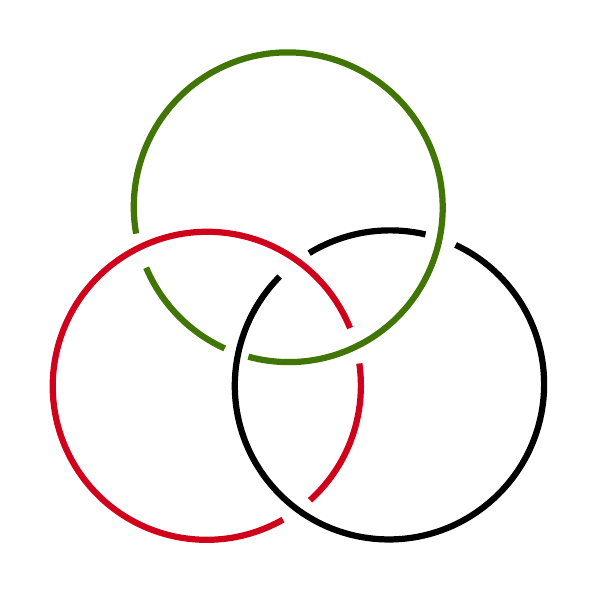
\begin{tikzpicture}[x=0.75pt,y=0.75pt,yscale=-1,xscale=1]
%uncomment if require: \path (0,300); %set diagram left start at 0, and has height of 300

%Shape: Arc [id:dp5841759180684423] 
\draw  [draw opacity=0][line width=2.25]  (290.27,165.55) .. controls (273.28,157.84) and (259.7,143.9) .. (252.41,126.63) -- (320.87,97.51) -- cycle ; \draw  [color={rgb, 255:red, 65; green, 117; blue, 5 }  ,draw opacity=1 ][line width=2.25]  (290.27,165.55) .. controls (273.28,157.84) and (259.7,143.9) .. (252.41,126.63) ;  
%Shape: Arc [id:dp7577998399786959] 
\draw  [draw opacity=0][line width=2.25]  (401.49,115.68) .. controls (411.67,120.44) and (420.91,127.58) .. (428.32,137) .. controls (453.68,169.27) and (447.97,216.08) .. (415.56,241.55) .. controls (383.16,267.03) and (336.33,261.52) .. (310.96,229.25) .. controls (287.54,199.45) and (290.62,157.26) .. (316.74,130.91) -- (369.64,183.13) -- cycle ; \draw  [color={rgb, 255:red, 0; green, 0; blue, 0 }  ,draw opacity=1 ][line width=2.25]  (401.49,115.68) .. controls (411.67,120.44) and (420.91,127.58) .. (428.32,137) .. controls (453.68,169.27) and (447.97,216.08) .. (415.56,241.55) .. controls (383.16,267.03) and (336.33,261.52) .. (310.96,229.25) .. controls (287.54,199.45) and (290.62,157.26) .. (316.74,130.91) ;  
%Shape: Arc [id:dp896095108426711] 
\draw  [draw opacity=0][line width=2.25]  (247.58,110.23) .. controls (241.88,77.87) and (258.12,44.5) .. (289.17,29.93) .. controls (326.35,12.5) and (370.67,28.62) .. (388.18,65.94) .. controls (405.69,103.27) and (389.75,147.66) .. (352.57,165.1) .. controls (336.02,172.86) and (318.05,173.97) .. (301.66,169.52) -- (320.87,97.51) -- cycle ; \draw  [color={rgb, 255:red, 65; green, 117; blue, 5 }  ,draw opacity=1 ][line width=2.25]  (247.58,110.23) .. controls (241.88,77.87) and (258.12,44.5) .. (289.17,29.93) .. controls (326.35,12.5) and (370.67,28.62) .. (388.18,65.94) .. controls (405.69,103.27) and (389.75,147.66) .. (352.57,165.1) .. controls (336.02,172.86) and (318.05,173.97) .. (301.66,169.52) ;  
%Shape: Arc [id:dp5765147440419169] 
\draw  [draw opacity=0][line width=2.25]  (318.33,248.02) .. controls (282.68,268.27) and (237.38,255.9) .. (217.12,220.36) .. controls (196.83,184.78) and (209.3,139.45) .. (244.97,119.12) .. controls (280.64,98.78) and (326,111.14) .. (346.28,146.72) .. controls (347.96,149.66) and (349.41,152.67) .. (350.65,155.72) -- (281.7,183.54) -- cycle ; \draw  [color={rgb, 255:red, 208; green, 2; blue, 27 }  ,draw opacity=1 ][line width=2.25]  (318.33,248.02) .. controls (282.68,268.27) and (237.38,255.9) .. (217.12,220.36) .. controls (196.83,184.78) and (209.3,139.45) .. (244.97,119.12) .. controls (280.64,98.78) and (326,111.14) .. (346.28,146.72) .. controls (347.96,149.66) and (349.41,152.67) .. (350.65,155.72) ;  
%Shape: Arc [id:dp9828413593386676] 
\draw  [draw opacity=0][line width=2.25]  (330.95,119.62) .. controls (347.94,109.22) and (368.18,106.21) .. (387.01,110.62) -- (369.64,183.13) -- cycle ; \draw  [color={rgb, 255:red, 0; green, 0; blue, 0 }  ,draw opacity=1 ][line width=2.25]  (330.95,119.62) .. controls (347.94,109.22) and (368.18,106.21) .. (387.01,110.62) ;  
%Shape: Arc [id:dp23316225635631627] 
\draw  [draw opacity=0][line width=2.25]  (355.12,172.79) .. controls (356.17,180.07) and (356.16,187.63) .. (354.93,195.28) .. controls (352.14,212.7) and (343.51,227.73) .. (331.38,238.69) -- (281.7,183.54) -- cycle ; \draw  [color={rgb, 255:red, 208; green, 2; blue, 27 }  ,draw opacity=1 ][line width=2.25]  (355.12,172.79) .. controls (356.17,180.07) and (356.16,187.63) .. (354.93,195.28) .. controls (352.14,212.7) and (343.51,227.73) .. (331.38,238.69) ;  




\end{tikzpicture}
}
   \caption{3-Hopf Rings}
\end{figure}
\noindent
The above discussion demonstrates that an entangled quantum state can correspond to more than one knot configuration if we define cutting of knot to be equivalent to measurement in a particular basis. As observables to be measured can be chosen in many different ways(for example spin can be measured along different directions in space), there seems to be no unique quantum process that corresponds to the mathematical act of cutting a knot. \\[0.3cm]
Now we investigate another three particle state, known as the $\ket{W}$ state, given by:
\[
\ket{\mathrm{W}} = \frac{1}{\sqrt{3}} (\ket{001}+\ket{010}+\ket{100}) 
\]
We measure spin of the first particle in z-direction. The outcome is $\frac{\hbar}{2}$ with probaility $\frac{2}{3}$, and $-\frac{\hbar}{2}$ with probability $\frac{1}{3}$.\\[0.2cm]
In the former case, after measurement, particles 2 and 3 are in state $\frac{1}{\sqrt{2}}(\ket{01}+\ket{10})$. This state is one of the Bell States and hence, maximally entangled. These can be modelled by 3-Hopf rings.\\[0.3cm] In the latter case, they are separable after the measurement and therefore modelled by Borromean rings.\\[0.3cm]
Thus we see that the $\ket{W}$ state can be modeled by Borromean rings with probability $\frac{1}{3}$ and by 3-Hopf rings with probability $\frac{2}{3}$.\\[0.3cm]
Aravind writes about one more linked 3-knots, where the middle ring in linked to the outer two rings, which are not connected to each other (we will call it the \textit{3-chain}). He shows that there exists a state corresponding to this link configuration.
\begin{figure}[H]
    \centering
   \scalebox{0.8}{ 

\tikzset{every picture/.style={line width=0.75pt}} %set default line width to 0.75pt        

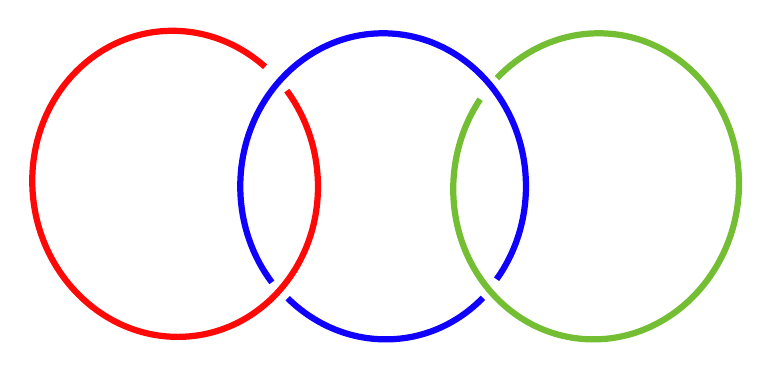
\begin{tikzpicture}[x=0.75pt,y=0.75pt,yscale=-1,xscale=1]
%uncomment if require: \path (0,300); %set diagram left start at 0, and has height of 300

%Shape: Arc [id:dp45545170377512756] 
\draw  [draw opacity=0][line width=2.25]  (234.67,185.2) .. controls (225.14,172.55) and (219.44,156.46) .. (219.44,138.93) .. controls (219.44,98.21) and (250.25,65.2) .. (288.26,65.2) .. controls (326.26,65.2) and (357.08,98.21) .. (357.08,138.93) .. controls (357.08,155.77) and (351.81,171.29) .. (342.94,183.71) -- (288.26,138.93) -- cycle ; \draw  [color={rgb, 255:red, 15; green, 0; blue, 255 }  ,draw opacity=1 ][line width=2.25]  (234.67,185.2) .. controls (225.14,172.55) and (219.44,156.46) .. (219.44,138.93) .. controls (219.44,98.21) and (250.25,65.2) .. (288.26,65.2) .. controls (326.26,65.2) and (357.08,98.21) .. (357.08,138.93) .. controls (357.08,155.77) and (351.81,171.29) .. (342.94,183.71) ;  
%Shape: Arc [id:dp43179396468586795] 
\draw  [draw opacity=0][line width=2.25]  (336.36,192.63) .. controls (324.26,205.05) and (307.81,212.67) .. (289.56,212.67) .. controls (271.41,212.67) and (254.78,205.14) .. (242.27,192.85) -- (288.26,138.93) -- cycle ; \draw  [color={rgb, 255:red, 15; green, 0; blue, 255 }  ,draw opacity=1 ][line width=2.25]  (336.36,192.63) .. controls (324.26,205.05) and (307.81,212.67) .. (289.56,212.67) .. controls (271.41,212.67) and (254.78,205.14) .. (242.27,192.85) ;  
%Shape: Arc [id:dp1272193908857524] 
\draw  [draw opacity=0][line width=2.25]  (241.85,92.84) .. controls (250.99,105.27) and (256.56,120.84) .. (256.86,137.73) .. controls (257.58,178.46) and (227.35,211.47) .. (189.34,211.47) .. controls (151.34,211.47) and (119.94,178.46) .. (119.23,137.73) .. controls (118.51,97.01) and (148.74,64) .. (186.74,64) .. controls (203.64,64) and (219.23,70.53) .. (231.4,81.35) -- (188.04,137.73) -- cycle ; \draw  [color={rgb, 255:red, 255; green, 8; blue, 8 }  ,draw opacity=1 ][line width=2.25]  (241.85,92.84) .. controls (250.99,105.27) and (256.56,120.84) .. (256.86,137.73) .. controls (257.58,178.46) and (227.35,211.47) .. (189.34,211.47) .. controls (151.34,211.47) and (119.94,178.46) .. (119.23,137.73) .. controls (118.51,97.01) and (148.74,64) .. (186.74,64) .. controls (203.64,64) and (219.23,70.53) .. (231.4,81.35) ;  
%Shape: Arc [id:dp33396414047455336] 
\draw  [draw opacity=0][line width=2.25]  (335.01,96.98) .. controls (327.1,108.89) and (322.33,123.35) .. (322.06,138.93) .. controls (321.34,179.65) and (351.57,212.67) .. (389.58,212.67) .. controls (427.59,212.67) and (458.99,179.65) .. (459.71,138.93) .. controls (460.43,98.21) and (430.19,65.2) .. (392.18,65.2) .. controls (373.16,65.2) and (355.8,73.46) .. (343.11,86.82) -- (390.88,138.93) -- cycle ; \draw  [color={rgb, 255:red, 115; green, 190; blue, 50 }  ,draw opacity=1 ][line width=2.25]  (335.01,96.98) .. controls (327.1,108.89) and (322.33,123.35) .. (322.06,138.93) .. controls (321.34,179.65) and (351.57,212.67) .. (389.58,212.67) .. controls (427.59,212.67) and (458.99,179.65) .. (459.71,138.93) .. controls (460.43,98.21) and (430.19,65.2) .. (392.18,65.2) .. controls (373.16,65.2) and (355.8,73.46) .. (343.11,86.82) ;  




\end{tikzpicture}
}
   \caption{3-chain}
\end{figure}
Notice that in previous sections, we started with a multi-particle quantum state, and checked how it behaves under various measurements and partial traces. Then, we tried to find a suitable link configuration but here we do just the reverse. 
Consider the state:
\[
\ket{\Psi} = \frac{1}{\sqrt{2}} (\ket{0++}+\ket{1--})
\]
We will show that this state can be modelled appropriately by the 3-chain.

\begin{align*}
    \ket{\Psi} &= \frac{1}{\sqrt{2}} \left[ \left( \ket{0} \otimes \frac{\ket{0} + \ket{1}}{\sqrt{2}} \otimes \frac{\ket{0} + \ket{1}}{\sqrt{2}} \right) + \left( \ket{1} \otimes \frac{\ket{0} - \ket{1}}{\sqrt{2}} \otimes \frac{\ket{0} - \ket{1}}{\sqrt{2}} \right) \right] \\[0.4cm]
    &= \frac{1}{\sqrt{2}} \left[ \frac{1}{\sqrt{2}} \left( \ket{00+} + \ket{01+} \right) + \frac{1}{\sqrt{2}} \left( \ket{10-} - \ket{11-} \right) \right] \\[0.4cm]
    &=\frac{\ket{0}_2}{\sqrt{2}}\brac{\frac{\ket{0}_1\ket{+}_3 +\ket{1}_1\ket{-}_3}{\sqrt{2}}}+\frac{\ket{1}_2}{\sqrt{2}}\brac{\frac{\ket{0}_1\ket{+}_3 -\ket{1}_1\ket{-}_3}{\sqrt{2}}}  \\[0.4cm]
    &= \frac{\ket{0}_3}{\sqrt{2}}\brac{\frac{\ket{0}_1\ket{+}_2 +\ket{1}_1\ket{-}_2}{\sqrt{2}}}+\frac{\ket{1}_3}{\sqrt{2}}\brac{\frac{\ket{0}_1\ket{+}_2 -\ket{1}_1\ket{-}_2}{\sqrt{2}}} \quad \text{[Changing $2\leftrightarrow 3$ since symmetric]}
    \end{align*}

Another alternate way of writing the same state is:
\[
\ket{\Psi} = \frac{\ket{+}_1}{\sqrt{2}}\brac{\frac{\ket{+}_2\ket{+}_3 +\ket{-}_2\ket{-}_3}{\sqrt{2}}}+\frac{\ket{-}_1}{\sqrt{2}}\brac{\frac{\ket{+}_2\ket{+}_3 -\ket{-}_1\ket{-}_3}{\sqrt{2}}}
\]



Now, we measure spin of the three particles in z-direction:
\begin{itemize}

    \item Measure spin of 1: After the measuement, particles 2 and 3 are in state $\ket{+}_2\ket{+}_3 \text{ or }\ket{-}_2\ket{-}_3$. Thus, irrespective of the outcome, particles 2 and 3 are disentangled. 
    
    \item Measure spin of 2: After the measurement, particles 1 and 3 are in state $\ket{0}_1\ket{+}_3 +\ket{1}_1\ket{-}_3\text{ or } \ket{0}_1\ket{+}_3 -\ket{1}_1\ket{-}_3$. Thus, irrespective of the outcome, particles 1 and 3 are maximally entangled (Using equation $(*_1)$). 
    
    \item Measure spin of 3: After the measurement, particles 1 and 2 are in state $\ket{0}_1\ket{+}_2 +\ket{1}_1\ket{-}_2\text{ or }\ket{0}_1\ket{+}_2 -\ket{1}_1\ket{-}_2$. Thus, irrespective of the outcome, particles 1 and 2 are maximally entangled (Using equation $(*_2)$).
    
\end{itemize}
Aravind concludes his paper by noting the low possiblility to develop the analogy between entangled quantum states and knot configurations in any systematic fashion. A part of the difficulty arises because there is no single quantum process that corresponds to the mathematical act of cutting a knot. It appears very unlikely that the classification of knot configurations could have any systematic application or utility in the study of entangled quantum states.\\[0.3cm]
However he listed some possible use cases for this classification scheme:
\begin{itemize}
    \item If some complicated knot becomes equivalent to the unknot, then there is a possibility that the corresponding quantum state is separable in some basis.
    \item Two equivalent knots might imply that two entangled states (represented by those knots) are equivalent, only written in different bases.
    \item More entangled knots might represent a higher degree of entanglement, leading to some topological entanglement measure.
\end{itemize}
We now consider another paper by Sugita (2007) extrapolating Aravind's work. Sugita introduced a basis-independent correspondence between quantum states and links. In the
 following, we consider composite systems consisting of qubits, and associate a ring
 with a qubit. Two entangled qubits are represented by two entangled rings, and two separable qubits are represented by two unentangled rings.\\[0.3cm] If we associate the measurement with cutting of the corresponding ring (as was done by Aravind), then the correspondence  depends on the choice of measurement basis. Instead, in this paper, partial trace was used instead of measurement as a counterpart of `cutting of a link'. Physically speaking, it means that the corresponding qubit is ignored and we focus only on the remaining qubits.\\[0.3cm]
We start with the 3-particle GHZ state and trace out qubit A from the original density matrix for the entire system, leading to the reduced density operator:
\[
\hat{\rho}_{bc} = \Tr_a\hat{\rho} = \frac{1}{2}(\ket{00}\bra{00}+\ket{11}\bra{11})
\]
which is a separable mixed state, as shown before. Therefore this state corresponds to the Borromean ring. Thus we can establish a connection between qubits and rings in a basis-independent way, since partial trace requires us to find trace, which is basis-independent.\\[0.3cm]
Now we will see how the correspondence between tracing out a particle (finding the reduced density operator) and cutting of the corresponding ring gives a natural basis-independent way to associate topological rings to quantum entangled states. We have the $\ket{W}$ state as follows:
\[
\ket{\mathrm{W}} = \frac{1}{\sqrt{3}}\brac{\ket{001}+\ket{010}+\ket{100}}
\]
The density operator for the W state is then $$\rho = \ket{\mathrm{W}}\bra{\mathrm{W}}$$
Using the partial trace with respect to particle A, we find the reduced density operator for particles B and C: 
\begin{align*}
    \rho_{BC} &= \tensor[_A]{\bra{0}\rho\ket{0}}{_A} + \tensor[_A]{\bra{1}\rho\ket{1}}{_A}
\end{align*}
From this calculation we can find the reduced density operator of particles 2 and 3 to be:
\[
 \rho_{BC} = \frac{1}{3}\brac{\ket{00}\bra{00}+\ket{01}\bra{10}+\ket{10}\bra{10}+\ket{01}\bra{01}+\ket{10}\bra{01}}
\]
Define
\[
\ket{\Psi} = \ket{01}+\ket{10}\Rightarrow \rho_{BC} = \frac{1}{3}\ket{00}\bra{00}+\frac{1}{3}\ket{\Psi}\bra{\Psi}
\]


Note that $\ket{\Psi}$ is not normalized.
Let $\ket{\Psi}_N$ denote normalized $\ket{\Psi}$
\[
\ket{\Psi}_N = \frac{1}{\sqrt{2}}(\ket{01}+\ket{10})
\]
\[
\Rightarrow \ket{\Psi}_N\bra{\Psi}_N= \frac{1}{2}\ket{\Psi}\bra{\Psi}
\Rightarrow \ket{\Psi}\bra{\Psi} = 2\ket{\Psi}_N\bra{\Psi}_N
\]
Thus 
\[
\rho^{BC} = \frac{1}{3}\ket{00}\bra{00}+\frac{2}{3}\ket{\Psi}_N\bra{\Psi}_N
\]
Here, $\ket{00}$ and $\ket{\Psi}_N$ are normalized. Hence $\rho^{BC}$ is a mixed state. Sugita uses the Concurrence Test\cite{Wootters1998} for separability. The concurrence of a density operator is defined as:
$$\mathrm{C}(\rho) = \max\{0,\lambda_1-\lambda_2-\lambda_3-\lambda_4\}$$
%  We can perform the Concurrence test. It turns out that $C(\rho^{BC})>0$, thus B and C are entangled. Therefore this state can be modelled by 3-Hopf rings.
Here $\lambda_i$ are the square root of the eigenvalues, in decreasing order, of the non-Hermitian matrix $\tilde{\rho}\rho$ where $\tilde{\rho}$ is defined by:
$$\tilde{\rho} = (\sigma_y\otimes\sigma_y)\rho^*(\sigma_y\otimes\sigma_y)$$
According to the Concurrence test, a state represented by the density operator $\rho$ is separable iff $C(\rho)=0$. \\[0.3cm]
For the above reduced density matrix, we find:
\begin{equation*}
    \tilde{\rho} =
    \left[
    \begin{array}{cccc}
    0.0 & 0.0 & 0.0 & 0.0 \\
    0.0 & 0.333 & 0.333 & 0.0 \\
    0.0 & 0.333 & 0.333 & 0.0 \\
    0.0 & 0.0 & 0.0 & 0.333 \\
    \end{array}
    \right] \quad \text{and}\quad \tilde{\rho}\rho = 
        \left[
        \begin{array}{cccc}
        0.0 & 0.0 & 0.0 & 0.0 \\
        0.0 & 0.148 & 0.148 & 0.0 \\
        0.0 & 0.148 & 0.148 & 0.0 \\
        0.0 & 0.0 & 0.0 & 0.0 \\
        \end{array}
        \right]    
    \end{equation*}
    The eigenvalues of $\tilde{\rho}\rho$ are $0.444, 0.0,0.0,0.0$ and hence $\mathrm{C(\rho)} = 0.444$ which is positive and hence the state is entangled.\\[0.3cm]
Now we consider the 3-chain state:
\[
\ket{\Psi} = a\ket{000} + b\ket{+1+},  \text{ with } \ a,b \in \mathbb{R}, \  |a|^2+|b|^2=1
\]
Then the density matrix is obtained as:
\[
\rho^{ABC}=\ket{\Psi}\bra{\Psi} = |a|^2 (\ket{000}\bra{000})+|b|^2(\ket{+1+}\bra{+1+})
\]
Now we trace out B and find $\rho^{AC} $:

\[\rho^{AC} = \mathrm{tr}_B(\rho^{ABC})=|a|^2\mathrm{tr}_B(\ket{0}\bra{0}).(\ket{00}\bra{00}) + |b|^2\mathrm{tr}_B(\ket{1}\bra{1}).(\ket{++}\bra{++})\]
Recall that $\mathrm{tr}_B(\ket{0}\bra{0})$ = $\mathrm{tr}_B(\ket{1}\bra{1})$ = 1. 
Therefore $\rho^{AC}$ represents a mixed state. Note that it can be written as:
\[
    \rho^{AC} = |a|^2\ket{00}\bra{00}+|b|^2\ket{++}\bra{++}=|a|^2\ket{0}\bra{0}\otimes\ket{0}\bra{0}+|b|^2\ket{+}\bra{+}\otimes\ket{+}\bra{+}
\]
Thus, we see that $\rho^{AC}$ is also separable. 
Similarly, we have $\rho^{BC}$ and $\rho^{AB}$:

\[
\rho^{AB}=|a|^2\ket{00}\bra{00}+|b|^2\ket{+1}\bra{+1}
\]
\[
\rho^{BC}=|a|^2\ket{00}\bra{00}+|b|^2\ket{1+}\bra{1+}
\]
Let us now calculate the concurrence of $\rho^{AB}$ and $\rho^{BC}$. From the definition, we calculated: 
\begin{equation*}
    \rho_{ab} =
    \left[
    \begin{array}{cccc}
    a^{2} & \frac{1}{2} a b & 0 & \frac{1}{2} a b \\[0.3cm]
    \frac{1}{2} a b & \frac{1}{2} b^{2} & 0 & \frac{1}{2} b^{2} \\[0.3cm]
    0 & 0 & 0 & 0 \\[0.3cm]
    \frac{1}{2} a b & \frac{1}{2} b^{2} & 0 & \frac{1}{2} b^{2} \\[0.3cm]
    \end{array}
    \right]\quad \tilde{\rho}_{ab}\rho_{ab} = \frac{ab}{4}\left[
        \begin{array}{cccc}
        3 a b & 3 b^{2} & 0 & 3 b^{2} \\[0.5cm]
        0 & 0 & 0 & 0 \\[0.5cm]
        -3 a b & -3 b^{2} & 0 & -3 b^{2} \\[0.5cm]
        4 a^{2} & 3 a b & 0 & 3 a b \\[0.5cm]
        \end{array}
        \right]
    \end{equation*}

    \begin{equation*}\
        \rho_{bc} =
        \left[
        \begin{array}{cccc}
        a^{2} & 0 & \frac{1}{2} a b & \frac{1}{2} a b \\[0.3cm]
        0 & 0 & 0 & 0 \\[0.3cm]
        \frac{1}{2} a b & 0 & \frac{1}{2} b^{2} & \frac{1}{2} b^{2} \\[0.3cm]
        \frac{1}{2} a b & 0 & \frac{1}{2} b^{2} & \frac{1}{2} b^{2} \\[0.3cm]
        \end{array}
        \right] \quad \tilde{\rho}_{bc}\rho_{bc} =\frac{ab}{4}\left[
            \begin{array}{cccc}
            3 a b& 0 & 2 b^{2} & 2 b^{2} \\[0.5cm]
           3 a b & 0 & -2 b^{2} & -2 b^{2} \\[0.5cm]
            0 & 0 & 0 & 0 \\[0.5cm]
            4 a^{2} & 0 & 3 a b& 3 a b\\[0.5cm]
            \end{array}
            \right]
        \end{equation*}
\noindent
These matrices have the same eigenvalues (since the system is symmetric with respect to A and C). The eigenvalues are: $|ab|\frac{(1 + \sqrt{2})}{2},|ab| \frac{(\sqrt{2} - 1)}{2},0,0$. Thus the concurrence is: $$\mathrm{C(\rho)} = |ab|>0$$
\noindent
Calculating the concurrence reveals that $\rho_{ab}$ and $\rho_{bc}$ are not separable. Thus, BC and AB are still entangled. This is clearly mirrored in the 3-chain link configuration, in which A and C are the outer rings and B is the middle one. So, if B is cut (or in the language of Quantum mechanics, traced out) A and C are separable, they are not linked. However if either A or C are cut, then, other 2 are still linked.
%88888888888888888888888888888888888888


\section{Classification of Links: A Polynomial Approach}
\subsection{Formalism of the Link Polynomial}
There are a number of rules that should be satisfied in order for a certain polynomial to represent a valid link, as explained in the following:
\begin{itemize}
    \item{There must not be any repeated terms, i.e., no ring variable can have a power greater than 1, for example, aab,
    should not appear,as it represents superfluous information ;we already know that the ring a is linked to b from the product ab,so multiplying another a is redundant. So, one only needs to use terms where no variables are repeated.}
    \item{Each ring variable must appear at least once, as we will only be concerned with the case where all initial rings are linked.}
    \item{There must not be first-order terms, possibility of including single variable terms is not of interest to us, since it would mean that the ring is not linked to any other. no particular importance is given to any ring variable since no information is contained in the variables themselves. For example, the polynomials ab+ac and ab+bc represent the same link class.}
    \item{ Relabeling of variables is irrelevant.}
    \item{An n-variable monomial M is irrelevant if all of its variables are already present as an n-ring link of lesser-order  monomials built only with the variables of M, consider the case where a given polynomial contains the terms ab and ac, it is irrelevant if we further add the term abc, since all the letters of the latter term have already appeared in the smaller monomials. Indeed, one may check by
    setting each letter to zero independently, that the results of all possible cuts are equal for both ab + ac and ab+ ac+ abc, and so both polynomials must represent the same link class. However, ab + cd and ab+cd+abcd represent different link class as the former represents two links, with 2 knots each, the latter represents 4 rings are linked.}
\end{itemize}
These rules are sufficient to select the desired polynomials, corresponding to each distinct link class, for any number of rings.  By construction, any link can be associated to one and only one of these classes. 
\subsection{Obtaining a Link from an Entangled Quantum State}\label{link_from_state}

\subsection{Obtaining an Entangled Quantum State from a Link}\label{state_from_link}
In this section, we will see how we can obtain a link from a quantum state. This is in general a difficult task to obtain an entangled quantum states from the polynomial as the number of qubits increases. The process in the paper mentions an algorithm which provides an `incomplete' map betwee a given link and a quantum state. Using the procedure, the general structure of the quantum state can be obtained, however, some free coefficients remain which needs to be fixed computationally. Moreover, presently only mixed states satisfying the link can be obtained using this procedure. \\[0.3cm]
Note that although incomplete, the map is still useful since we can ascertain the structure of each state contained in the mixed state. That is, from a possibility of $2^N$ (for $N$ qubits, there are $2^N$ basis states, namely $\ket{0}, \ket{1}, \ldots \ket{2^N-1}$ where each ket is to be assumed in the binary representation) states, we are reducing it to a much smaller number. \\[0.3cm]
For this, we will use the GHZ type of state as a building block which are of the form:
\begin{align*}
    \ket{N^1} = \frac{1}{\sqrt{2}}\brac{\ket{0}^{\otimes N} + \ket{1}^{\otimes N}} \\
\end{align*}
Here $\ket{0}^{\otimes N}$ is the tensor product of $N$ number of $\ket{0}$ states, that is, $\ket{0}^{\otimes N} = \ket{\underbrace{0000\ldots0}_{\mathrm{N\ times}}}$. The state $\ket{N^1}$ is a maximally entangled state of $N$ qubits. The general algorithm to obtain a state from the link is as follows:
\begin{enumerate}
    \item Let a polynomial $P$ be given. Select a term of the given `link' polynomial, say $t$. 
    \item The term $t$ is then mapped to a state of the form $\ket{\mathrm{E_q}}\otimes\ket{\mathrm{S_q}}\otimes\ket{\mathrm{Q_d}}$ where: 
    \begin{itemize}
        \item $\ket{\mathrm{E_q}}$ is the entangled qubit of the GHZ type as specified above, associated to ring variables contained in $t$.
        \item $\ket{\mathrm{S_q}}$ is a separable qubit associated with ring variables not contained in $t$. There are a number of possibilities for this separable qubit and we have to find it computationally.
        \item $\ket{\mathrm{Q_d}}$ is a qudit state which is associated with an artifically introduced ring variable (which is alphabetically the next letter of the largest ring variable present). The states always starts from 0 for the first term and is increased by 1 for each successive term of the polynomial. This will later be traced out, hence is of less significance. 
    \end{itemize}
    \item The full state $\ket{\psi}$ is constructed by summing these individual states obtained for each term of the polynomial. 
    \item The full mixed state characterised by this polynomial is then obtained by tracing out the qudit state $\ket{\mathrm{Q_d}}$.
    $$\boxed{\hat{\rho}(P)=\frac{\Tr_d{\ket{\psi}\bra{\psi}}}{\Tr{\Tr_d{\ket{\psi}\bra{\psi}}}}}$$
\end{enumerate}
\begin{figure}[H]
    \centering 
   \scalebox{0.8}{ 

\tikzset{every picture/.style={line width=0.75pt}} %set default line width to 0.75pt        

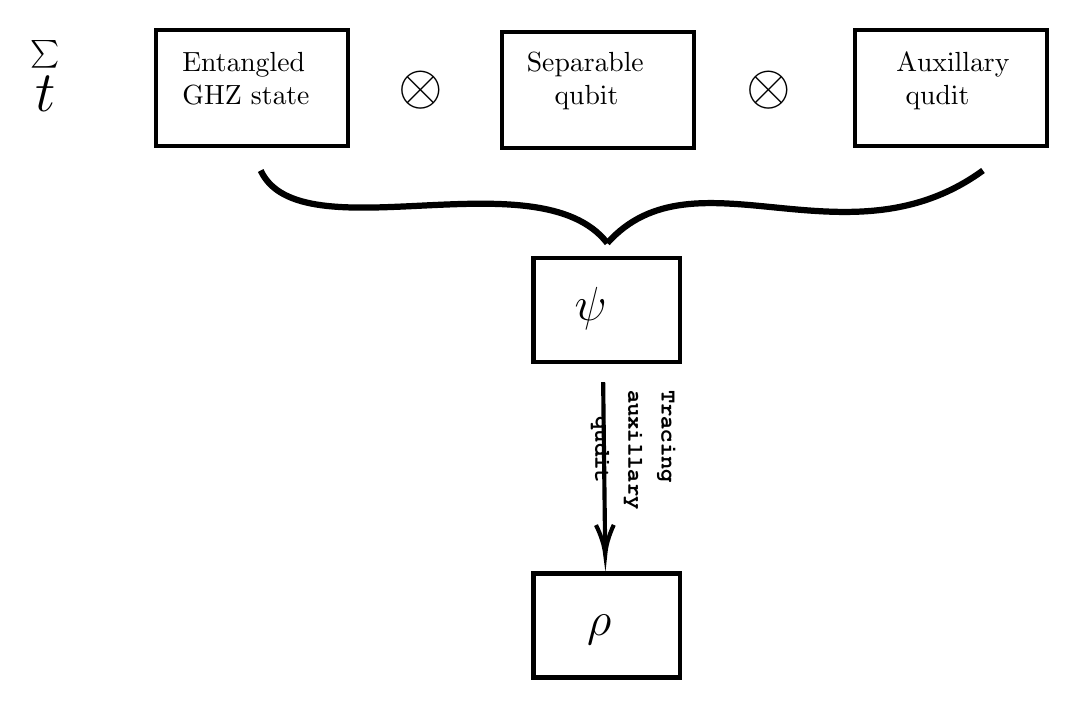
\begin{tikzpicture}[x=0.75pt,y=0.75pt,yscale=-1,xscale=1]
%uncomment if require: \path (0,418); %set diagram left start at 0, and has height of 418

%Shape: Rectangle [id:dp7294540182578855] 
\draw  [color={rgb, 255:red, 0; green, 0; blue, 0 }  ,draw opacity=1 ][fill={rgb, 255:red, 255; green, 255; blue, 255 }  ,fill opacity=1 ][line width=1.5]  (86.44,31.57) -- (178.88,31.57) -- (178.88,87.63) -- (86.44,87.63) -- cycle ;
%Shape: Rectangle [id:dp4761246648053713] 
\draw  [color={rgb, 255:red, 0; green, 0; blue, 0 }  ,draw opacity=1 ][fill={rgb, 255:red, 255; green, 255; blue, 255 }  ,fill opacity=1 ][line width=1.5]  (253.44,32.57) -- (345.88,32.57) -- (345.88,88.63) -- (253.44,88.63) -- cycle ;
%Shape: Rectangle [id:dp5375732459667567] 
\draw  [color={rgb, 255:red, 0; green, 0; blue, 0 }  ,draw opacity=1 ][fill={rgb, 255:red, 255; green, 255; blue, 255 }  ,fill opacity=1 ][line width=1.5]  (423.44,31.57) -- (515.88,31.57) -- (515.88,87.63) -- (423.44,87.63) -- cycle ;
%Shape: Rectangle [id:dp8708856606447273] 
\draw  [color={rgb, 255:red, 0; green, 0; blue, 0 }  ,draw opacity=1 ][fill={rgb, 255:red, 255; green, 255; blue, 255 }  ,fill opacity=1 ][line width=1.5]  (268.44,141.57) -- (339,141.57) -- (339,191.62) -- (268.44,191.62) -- cycle ;
%Curve Lines [id:da5387806644578281] 
\draw [line width=2.25]    (137,99.38) .. controls (156,140.38) and (271,91.77) .. (304,134.38) ;
%Curve Lines [id:da3604580216133906] 
\draw [line width=2.25]    (304,134.38) .. controls (346,87.38) and (419,147.38) .. (485,99.38) ;
%Straight Lines [id:da04531485758321774] 
\draw [line width=1.5]    (302,201.38) -- (302.96,281.38) ;
\draw [shift={(303,284.38)}, rotate = 269.31] [color={rgb, 255:red, 0; green, 0; blue, 0 }  ][line width=1.5]    (14.21,-4.28) .. controls (9.04,-1.82) and (4.3,-0.39) .. (0,0) .. controls (4.3,0.39) and (9.04,1.82) .. (14.21,4.28)   ;
%Shape: Rectangle [id:dp4350486178723396] 
\draw  [color={rgb, 255:red, 0; green, 0; blue, 0 }  ,draw opacity=1 ][fill={rgb, 255:red, 255; green, 255; blue, 255 }  ,fill opacity=1 ][line width=1.5]  (268.44,293.57) -- (339,293.57) -- (339,343.62) -- (268.44,343.62) -- cycle ;

% Text Node
\draw (97.98,41) node [anchor=north west][inner sep=0.75pt]   [align=left] {Entangled\\GHZ state};
% Text Node
\draw (263.98,41) node [anchor=north west][inner sep=0.75pt]   [align=left] {Separable\\ \ \ \ qubit};
% Text Node
\draw (441.98,41) node [anchor=north west][inner sep=0.75pt]   [align=left] {Auxillary \\ \ qudit};
% Text Node
\draw (287,154.4) node [anchor=north west][inner sep=0.75pt]  [font=\LARGE]  {$\ket{\psi }$};
% Text Node
\draw (202,50.4) node [anchor=north west][inner sep=0.75pt]  [font=\huge]  {$\mathlarger{\otimes} $};
% Text Node
\draw (370,50) node [anchor=north west][inner sep=0.75pt]  [font=\huge]  {$\mathbf{\otimes} $};
% Text Node
\draw (293,312.4) node [anchor=north west][inner sep=0.75pt]  [font=\LARGE]  {$\rho $};
% Text Node
\draw (338.5,203.88) node [anchor=north west][inner sep=0.75pt]  [rotate=-90] [align=left] {{\footnotesize {\fontfamily{pcr}\selectfont  \textbf{Tracing} }}\\{\footnotesize {\fontfamily{pcr}\selectfont \textbf{auxillary}}}\\{\footnotesize {\fontfamily{pcr}\selectfont  \ \ \textbf{qudit}}}};
% Text Node
\draw (25,35.4) node [anchor=north west][inner sep=0.75pt]  [font=\Huge]  {$\sum \limits_{{t}}$};


\end{tikzpicture}
}
   \caption{A schematic diagram of the algorithm}
\end{figure}
\textbf{Example demonstrating the algorithm:} \\[0.3cm]
We will see a simple example of the algorithm to obtain a state from a link. Consider the polynomial $P(a,b,c) = ab+ac$. This is a three-ring link. 
\begin{itemize}
    \item Let us choose the term $t = ab$. This term has two ring variables thus we will associate a two qubit GHZ type of state to $\ket{\mathrm{E_q}}$. Thus, we have $\ket{\mathrm{E_q}} = \frac{1}{\sqrt{2}}\brac{\ket{00} + \ket{11}}\equiv \ket{2^1}_{ab}$. \\[0.3cm]Since the separable qubit has large possibility, we will denote it generally by $\ket{q_1}$ and this will be associated with the remaining ring variable which is $c$. Thus, $\ket{\mathrm{S_q}} = \ket{q_1}_c$. The remaining term is the qudit state which will be associated to $d$ (since $d$ is alphabetical successor of the largest ring variable $c$). Then we will have the full state:
\begin{align*}
    \ket{\psi_1} &= \ket{2^1}_{ab}\otimes\ket{q_1}_c\otimes\ket{0}_d 
\end{align*}
\item Now, let us choose the next term in the polynomial which is $t = ac$. Similar to above, to the entangled qubit we will associate the two qubit GHZ state, thus, $\ket{\mathrm{E_q}} = \frac{1}{\sqrt{2}}\brac{\ket{00} + \ket{11}}\equiv \ket{2^1}_{ac}$.\\[0.3cm] The separable qubit will be associated with the remaining ring variable $b$ and we will denote it by $\ket{q_2}_b$. The qudit state will be associated with $d$ which is the alphabetical successor of $c$ but this time we will use $\ket{1}_d$ as for each successive term, the qudit state increases to the next level. Thus, we have:
\begin{align*}
    \ket{\psi_2} &= \ket{2^1}_{ac}\otimes\ket{q_2}_b\otimes\ket{1}_d
\end{align*}
\item The full state $\ket{\psi}$ is then obtained by summing the two states obtained above with some coefficients:
\begin{align*}
    \ket{\psi} &= c_1\ket{\psi_1} + c_2\ket{\psi_2} \\
    &=c_1(\ket{2^1}_{ab}\otimes\ket{q_1}_c\otimes\ket{0}_d )+ c_2(\ket{2^1}_{ac}\otimes\ket{q_2}_b\otimes\ket{1}_d)
\end{align*}
Then we can trace out the qudit state $\ket{d}$ to obtain the density matrix of the ring variables:
$$\boxed{\hat{\rho}_{abc}=\frac{\Tr_d{\ket{\psi}\bra{\psi}}}{\Tr{\Tr_d{\ket{\psi}\bra{\psi}}}}} $$
\end{itemize}
\subsection{Applying to Three Qubit Systems}
As a demonstration, we will apply our algorithm to three qubit systems. Note that from the rules of the `link' polynomial, the possible basis terms for three qubit system are: $\{ab,ac,bc, abc\}$. Using this, four distinct classes of polynomials are possible:
\begin{align*}
    \mathrm{P_1(a,b,c)} &=\mathrm{abc} \\
   \mathrm{P_2(a,b,c)} &=\mathrm{ abc+ab} \\
   \mathrm{P_3(a,b,c)} &=\mathrm{ ab+ac} \\
   \mathrm{P_4(a,b,c)} &=\mathrm{ ab+ac+bc}
\end{align*}
\textbf{\large \texttt{3\textsuperscript{1}} Link Class} \\[0.3cm]
Let us start with the $3^1$ link class, which corresponds to the Borromean Link and is given by $\mathrm{P_1(a,b,c)= abc}$. Cutting any of $a,b$ or $c$ will lead to complete separabability and loss of entanglement. 
\begin{figure}[H]
    \centering
  

\tikzset{every picture/.style={line width=0.75pt}} %set default line width to 0.75pt        

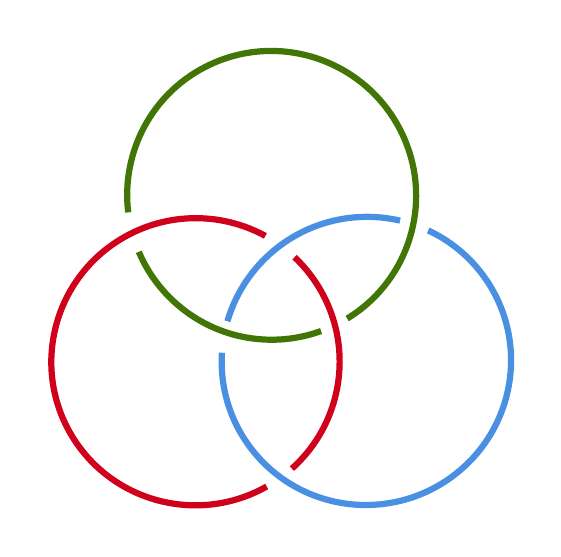
\begin{tikzpicture}[x=0.75pt,y=0.75pt,yscale=-1,xscale=1]
%uncomment if require: \path (0,300); %set diagram left start at 0, and has height of 300

%Shape: Arc [id:dp49278097545949884] 
\draw  [draw opacity=0][line width=2.25]  (328.62,163.73) .. controls (321.19,166.44) and (313.18,167.92) .. (304.82,167.92) .. controls (276.06,167.92) and (251.39,150.46) .. (240.8,125.56) -- (304.82,98.33) -- cycle ; \draw  [color={rgb, 255:red, 65; green, 117; blue, 5 }  ,draw opacity=1 ][line width=2.25]  (328.62,163.73) .. controls (321.19,166.44) and (313.18,167.92) .. (304.82,167.92) .. controls (276.06,167.92) and (251.39,150.46) .. (240.8,125.56) ;  
%Shape: Arc [id:dp7313937278600963] 
\draw  [draw opacity=0][line width=2.25]  (380.22,115.26) .. controls (389.75,119.69) and (398.4,126.36) .. (405.34,135.15) .. controls (429.07,165.23) and (423.73,208.87) .. (393.41,232.62) .. controls (363.09,256.37) and (319.27,251.24) .. (295.54,221.15) .. controls (284.6,207.29) and (279.84,190.54) .. (280.85,174.18) -- (350.44,178.15) -- cycle ; \draw  [color={rgb, 255:red, 74; green, 144; blue, 226 }  ,draw opacity=1 ][line width=2.25]  (380.22,115.26) .. controls (389.75,119.69) and (398.4,126.36) .. (405.34,135.15) .. controls (429.07,165.23) and (423.73,208.87) .. (393.41,232.62) .. controls (363.09,256.37) and (319.27,251.24) .. (295.54,221.15) .. controls (284.6,207.29) and (279.84,190.54) .. (280.85,174.18) ;  
%Shape: Arc [id:dp9082888658781946] 
\draw  [draw opacity=0][line width=2.25]  (235.71,106.58) .. controls (232.15,77.58) and (247.26,48.37) .. (275.16,35.34) .. controls (309.93,19.08) and (351.4,34.11) .. (367.78,68.91) .. controls (383.06,101.37) and (371.11,139.56) .. (341.2,157.73) -- (304.82,98.33) -- cycle ; \draw  [color={rgb, 255:red, 65; green, 117; blue, 5 }  ,draw opacity=1 ][line width=2.25]  (235.71,106.58) .. controls (232.15,77.58) and (247.26,48.37) .. (275.16,35.34) .. controls (309.93,19.08) and (351.4,34.11) .. (367.78,68.91) .. controls (383.06,101.37) and (371.11,139.56) .. (341.2,157.73) ;  
%Shape: Arc [id:dp7357603003827937] 
\draw  [draw opacity=0][line width=2.25]  (302.44,238.64) .. controls (269.08,257.52) and (226.71,245.99) .. (207.75,212.86) .. controls (188.77,179.69) and (200.44,137.44) .. (233.81,118.48) .. controls (255.62,106.09) and (281.32,106.72) .. (301.8,117.92) -- (268.17,178.53) -- cycle ; \draw  [color={rgb, 255:red, 208; green, 2; blue, 27 }  ,draw opacity=1 ][line width=2.25]  (302.44,238.64) .. controls (269.08,257.52) and (226.71,245.99) .. (207.75,212.86) .. controls (188.77,179.69) and (200.44,137.44) .. (233.81,118.48) .. controls (255.62,106.09) and (281.32,106.72) .. (301.8,117.92) ;  
%Shape: Arc [id:dp02993817280793909] 
\draw  [draw opacity=0][line width=2.25]  (283.51,159.01) .. controls (286.66,148.19) and (292.5,137.97) .. (301.03,129.39) .. controls (318.8,111.52) and (343.85,105.22) .. (366.69,110.55) -- (350.44,178.15) -- cycle ; \draw  [color={rgb, 255:red, 74; green, 144; blue, 226 }  ,draw opacity=1 ][line width=2.25]  (283.51,159.01) .. controls (286.66,148.19) and (292.5,137.97) .. (301.03,129.39) .. controls (318.8,111.52) and (343.85,105.22) .. (366.69,110.55) ;  
%Shape: Arc [id:dp6464277844327507] 
\draw  [draw opacity=0][line width=2.25]  (315.85,128.16) .. controls (331.94,143.37) and (340.46,165.99) .. (336.68,189.48) .. controls (334.06,205.76) and (325.96,219.8) .. (314.56,230.03) -- (268.17,178.53) -- cycle ; \draw  [color={rgb, 255:red, 208; green, 2; blue, 27 }  ,draw opacity=1 ][line width=2.25]  (315.85,128.16) .. controls (331.94,143.37) and (340.46,165.99) .. (336.68,189.48) .. controls (334.06,205.76) and (325.96,219.8) .. (314.56,230.03) ;  




\end{tikzpicture}
  
  \caption{The Borromean link, characterising the $3^1$ link class.}
\end{figure}
\noindent
We already know that on its own the GHZ state characterises the $3^1$ link, as discussed in the preceding works. Thus, we have the pure state:
$$\ket{3^1}_{abc} = \frac{1}{\sqrt{2}}\brac{\ket{000}_{abc}+\ket{111}_{abc}}$$\\[0.3cm]
The density matrix corresponding to the state is found to be:
\begin{equation*}
    \rho_{abc} =
    \left[
    \begin{array}{cccccccc}
    0.5 & 0.0 & 0.0 & 0.0 & 0.0 & 0.0 & 0.0 & 0.5 \\
    0.0 & 0.0 & 0.0 & 0.0 & 0.0 & 0.0 & 0.0 & 0.0 \\
    0.0 & 0.0 & 0.0 & 0.0 & 0.0 & 0.0 & 0.0 & 0.0 \\
    0.0 & 0.0 & 0.0 & 0.0 & 0.0 & 0.0 & 0.0 & 0.0 \\
    0.0 & 0.0 & 0.0 & 0.0 & 0.0 & 0.0 & 0.0 & 0.0 \\
    0.0 & 0.0 & 0.0 & 0.0 & 0.0 & 0.0 & 0.0 & 0.0 \\
    0.0 & 0.0 & 0.0 & 0.0 & 0.0 & 0.0 & 0.0 & 0.0 \\
    0.5 & 0.0 & 0.0 & 0.0 & 0.0 & 0.0 & 0.0 & 0.5 \\
    \end{array}
    \right]
    \end{equation*}
    The partial transpose with respect to any of the subsystem (since the polynomial is symmetric) is same and is given by:
    \begin{equation*}
        \rho^{T_a/T_b/T_c}_{abc} =
        \left[
        \begin{array}{cccccccc}
        0.5 & 0.0 & 0.0 & 0.0 & 0.0 & 0.0 & 0.0 & 0.0 \\
        0.0 & 0.0 & 0.0 & 0.0 & 0.0 & 0.0 & 0.0 & 0.0 \\
        0.0 & 0.0 & 0.0 & 0.0 & 0.0 & 0.0 & 0.0 & 0.0 \\
        0.0 & 0.0 & 0.0 & 0.0 & 0.5 & 0.0 & 0.0 & 0.0 \\
        0.0 & 0.0 & 0.0 & 0.5 & 0.0 & 0.0 & 0.0 & 0.0 \\
        0.0 & 0.0 & 0.0 & 0.0 & 0.0 & 0.0 & 0.0 & 0.0 \\
        0.0 & 0.0 & 0.0 & 0.0 & 0.0 & 0.0 & 0.0 & 0.0 \\
        0.0 & 0.0 & 0.0 & 0.0 & 0.0 & 0.0 & 0.0 & 0.5 \\
        \end{array}
        \right]
        \end{equation*}
        The eigenvalues corresponding to this matrix are $0.0, 0.5$ and $\mathbf{\mathbf{\mathcolor{red}{-0.5}}}$. Since there are negative eigenvalues, we can conclude that the system exhibits \textbf{tripartite entanglement} as a whole.\\[0.3cm]
        Now, let us reduce the system by tracing out one of the variable. Since the polynomial is symmetric, we can choose any of the variable to trace out, say $c$. The reduced density matrix is given by:
        \begin{equation*}
            \rho_{ab}
            \left[
            \begin{array}{cccc}
            0.5 & 0.0 & 0.0 & 0.0 \\
            0.0 & 0.0 & 0.0 & 0.0 \\
            0.0 & 0.0 & 0.0 & 0.0 \\
            0.0 & 0.0 & 0.0 & 0.5 \\
            \end{array}
            \right]
            \end{equation*} 
            The partial transpose with respect to $a$ or $b$ results in the same above matrix which have eigenvalues $0.5$ and $0.0$ which are all positive, thus concluding the absence of any entanglement in the system. This is consistent with the fact that for the Borromean link, cutting any link will result in complete separability of the links.
           \begin{figure}[H]
            \centering 
           \scalebox{0.8}{ 

\tikzset{every picture/.style={line width=0.75pt}} %set default line width to 0.75pt        

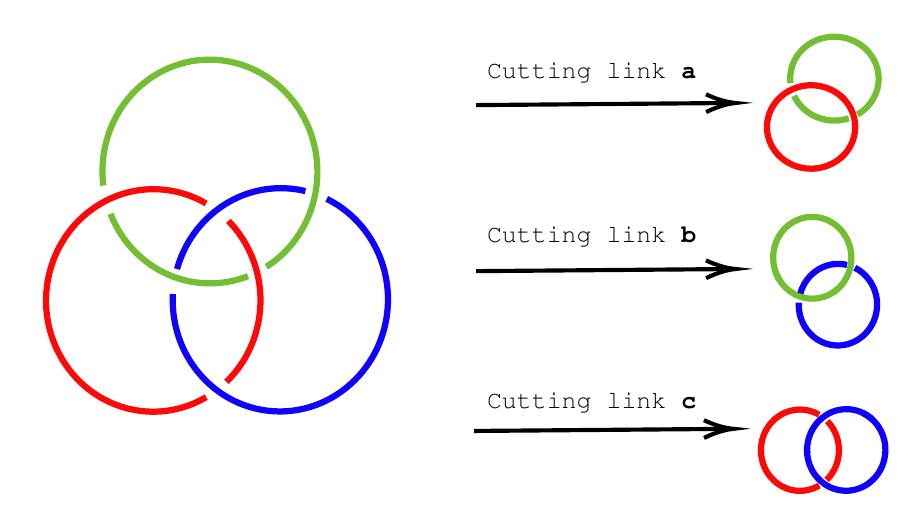
\begin{tikzpicture}[x=0.75pt,y=0.75pt,yscale=-1,xscale=1]
%uncomment if require: \path (0,284); %set diagram left start at 0, and has height of 284

%Shape: Arc [id:dp7197526417869784] 
\draw  [draw opacity=0][line width=2.25]  (174.11,165.4) .. controls (168.4,167.66) and (162.22,168.89) .. (155.76,168.89) .. controls (134.1,168.89) and (115.56,155.03) .. (107.85,135.36) -- (155.76,114.98) -- cycle ; \draw  [color={rgb, 255:red, 115; green, 190; blue, 50 }  ,draw opacity=1 ][line width=2.25]  (174.11,165.4) .. controls (168.4,167.66) and (162.22,168.89) .. (155.76,168.89) .. controls (134.1,168.89) and (115.56,155.03) .. (107.85,135.36) ;  
%Shape: Arc [id:dp4959572015620983] 
\draw  [draw opacity=0][line width=2.25]  (212.03,128.19) .. controls (219.04,131.63) and (225.41,136.76) .. (230.52,143.51) .. controls (248.18,166.81) and (244.2,200.62) .. (221.65,219.02) .. controls (199.1,237.42) and (166.51,233.45) .. (148.85,210.14) .. controls (140.77,199.47) and (137.22,186.61) .. (137.91,174.02) -- (189.69,176.82) -- cycle ; \draw  [color={rgb, 255:red, 15; green, 0; blue, 255 }  ,draw opacity=1 ][line width=2.25]  (212.03,128.19) .. controls (219.04,131.63) and (225.41,136.76) .. (230.52,143.51) .. controls (248.18,166.81) and (244.2,200.62) .. (221.65,219.02) .. controls (199.1,237.42) and (166.51,233.45) .. (148.85,210.14) .. controls (140.77,199.47) and (137.22,186.61) .. (137.91,174.02) ;  
%Shape: Arc [id:dp007665051622153252] 
\draw  [draw opacity=0][line width=2.25]  (104.41,121.78) .. controls (101.57,99.17) and (112.82,76.34) .. (133.7,66.17) .. controls (159.56,53.58) and (190.4,65.23) .. (202.59,92.18) .. controls (213.93,117.29) and (205.1,146.81) .. (182.94,160.93) -- (155.76,114.98) -- cycle ; \draw  [color={rgb, 255:red, 115; green, 190; blue, 50 }  ,draw opacity=1 ][line width=2.25]  (104.41,121.78) .. controls (101.57,99.17) and (112.82,76.34) .. (133.7,66.17) .. controls (159.56,53.58) and (190.4,65.23) .. (202.59,92.18) .. controls (213.93,117.29) and (205.1,146.81) .. (182.94,160.93) ;  
%Shape: Arc [id:dp9373017253564936] 
\draw  [draw opacity=0][line width=2.25]  (153.99,223.69) .. controls (129.19,238.32) and (97.67,229.38) .. (83.57,203.71) .. controls (69.45,178.02) and (78.12,145.28) .. (102.93,130.59) .. controls (119.3,120.9) and (138.61,121.49) .. (153.91,130.39) -- (128.5,177.12) -- cycle ; \draw  [color={rgb, 255:red, 255; green, 8; blue, 8 }  ,draw opacity=1 ][line width=2.25]  (153.99,223.69) .. controls (129.19,238.32) and (97.67,229.38) .. (83.57,203.71) .. controls (69.45,178.02) and (78.12,145.28) .. (102.93,130.59) .. controls (119.3,120.9) and (138.61,121.49) .. (153.91,130.39) ;  
%Shape: Arc [id:dp0642631306360737] 
\draw  [draw opacity=0][line width=2.25]  (139.91,162) .. controls (142.25,153.61) and (146.59,145.69) .. (152.94,139.05) .. controls (166.16,125.2) and (184.8,120.32) .. (201.78,124.45) -- (189.69,176.82) -- cycle ; \draw  [color={rgb, 255:red, 15; green, 0; blue, 255 }  ,draw opacity=1 ][line width=2.25]  (139.91,162) .. controls (142.25,153.61) and (146.59,145.69) .. (152.94,139.05) .. controls (166.16,125.2) and (184.8,120.32) .. (201.78,124.45) ;  
%Shape: Arc [id:dp3711468791957636] 
\draw  [draw opacity=0][line width=2.25]  (164.64,138.77) .. controls (176.16,150.54) and (182.21,167.75) .. (179.45,185.6) .. controls (177.56,197.85) and (171.82,208.47) .. (163.72,216.33) -- (128.5,177.12) -- cycle ; \draw  [color={rgb, 255:red, 255; green, 8; blue, 8 }  ,draw opacity=1 ][line width=2.25]  (164.64,138.77) .. controls (176.16,150.54) and (182.21,167.75) .. (179.45,185.6) .. controls (177.56,197.85) and (171.82,208.47) .. (163.72,216.33) ;  
%Straight Lines [id:da8108728397872645] 
\draw [line width=1.5]    (284,83) -- (327.98,82.64) -- (406,81.99) ;
\draw [shift={(409,81.97)}, rotate = 179.53] [color={rgb, 255:red, 0; green, 0; blue, 0 }  ][line width=1.5]    (14.21,-4.28) .. controls (9.04,-1.82) and (4.3,-0.39) .. (0,0) .. controls (4.3,0.39) and (9.04,1.82) .. (14.21,4.28)   ;
%Shape: Arc [id:dp6987925961310537] 
\draw  [draw opacity=0][line width=2.25]  (463.59,89.35) .. controls (461.41,90.07) and (459.07,90.46) .. (456.64,90.46) .. controls (447.98,90.46) and (440.52,85.55) .. (437.19,78.5) -- (456.64,70.24) -- cycle ; \draw  [color={rgb, 255:red, 115; green, 190; blue, 50 }  ,draw opacity=1 ][line width=2.25]  (463.59,89.35) .. controls (461.41,90.07) and (459.07,90.46) .. (456.64,90.46) .. controls (447.98,90.46) and (440.52,85.55) .. (437.19,78.5) ;  
%Shape: Arc [id:dp404500646035895] 
\draw  [draw opacity=0][line width=2.25]  (435.45,72.43) .. controls (434.46,64.06) and (439.08,55.69) .. (447.55,51.93) .. controls (458.2,47.2) and (470.9,51.57) .. (475.92,61.68) .. controls (480.61,71.14) and (476.92,82.27) .. (467.71,87.54) -- (456.64,70.24) -- cycle ; \draw  [color={rgb, 255:red, 115; green, 190; blue, 50 }  ,draw opacity=1 ][line width=2.25]  (435.45,72.43) .. controls (434.46,64.06) and (439.08,55.69) .. (447.55,51.93) .. controls (458.2,47.2) and (470.9,51.57) .. (475.92,61.68) .. controls (480.61,71.14) and (476.92,82.27) .. (467.71,87.54) ;  
%Shape: Arc [id:dp24258786153750556] 
\draw  [draw opacity=0][line width=2.25]  (461.17,107.03) .. controls (459.7,108.57) and (457.95,109.91) .. (455.94,110.99) .. controls (445.72,116.5) and (432.73,113.15) .. (426.91,103.52) .. controls (421.1,93.88) and (424.67,81.6) .. (434.89,76.09) .. controls (443.75,71.31) and (454.71,73.2) .. (461.25,80.08) -- (445.41,93.54) -- cycle ; \draw  [color={rgb, 255:red, 255; green, 8; blue, 8 }  ,draw opacity=1 ][line width=2.25]  (461.17,107.03) .. controls (459.7,108.57) and (457.95,109.91) .. (455.94,110.99) .. controls (445.72,116.5) and (432.73,113.15) .. (426.91,103.52) .. controls (421.1,93.88) and (424.67,81.6) .. (434.89,76.09) .. controls (443.75,71.31) and (454.71,73.2) .. (461.25,80.08) ;  
%Shape: Arc [id:dp2439073107835955] 
\draw  [draw opacity=0][line width=2.25]  (459.66,78.59) .. controls (464.81,83.01) and (467.58,89.73) .. (466.39,96.72) .. controls (465.56,101.63) and (462.93,105.83) .. (459.23,108.83) -- (445.41,93.54) -- cycle ; \draw  [color={rgb, 255:red, 255; green, 8; blue, 8 }  ,draw opacity=1 ][line width=2.25]  (459.66,78.59) .. controls (464.81,83.01) and (467.58,89.73) .. (466.39,96.72) .. controls (465.56,101.63) and (462.93,105.83) .. (459.23,108.83) ;  
%Straight Lines [id:da5533674689620419] 
\draw [line width=1.5]    (284,163) -- (327.98,162.64) -- (406,161.99) ;
\draw [shift={(409,161.97)}, rotate = 179.53] [color={rgb, 255:red, 0; green, 0; blue, 0 }  ][line width=1.5]    (14.21,-4.28) .. controls (9.04,-1.82) and (4.3,-0.39) .. (0,0) .. controls (4.3,0.39) and (9.04,1.82) .. (14.21,4.28)   ;
%Shape: Arc [id:dp14412002029410176] 
\draw  [draw opacity=0][line width=2.25]  (458.52,171.24) .. controls (455.19,174.36) and (450.79,176.26) .. (445.97,176.26) .. controls (438.08,176.26) and (431.32,171.18) .. (428.52,163.97) -- (445.97,156.55) -- cycle ; \draw  [color={rgb, 255:red, 115; green, 190; blue, 50 }  ,draw opacity=1 ][line width=2.25]  (458.52,171.24) .. controls (455.19,174.36) and (450.79,176.26) .. (445.97,176.26) .. controls (438.08,176.26) and (431.32,171.18) .. (428.52,163.97) ;  
%Shape: Arc [id:dp5310213203581242] 
\draw  [draw opacity=0][line width=2.25]  (466.46,161.38) .. controls (469.01,162.64) and (471.33,164.51) .. (473.18,166.98) .. controls (479.61,175.5) and (478.17,187.86) .. (469.96,194.58) .. controls (461.75,201.31) and (449.88,199.86) .. (443.45,191.34) .. controls (440.52,187.44) and (439.22,182.74) .. (439.47,178.15) -- (458.32,179.16) -- cycle ; \draw  [color={rgb, 255:red, 15; green, 0; blue, 255 }  ,draw opacity=1 ][line width=2.25]  (466.46,161.38) .. controls (469.01,162.64) and (471.33,164.51) .. (473.18,166.98) .. controls (479.61,175.5) and (478.17,187.86) .. (469.96,194.58) .. controls (461.75,201.31) and (449.88,199.86) .. (443.45,191.34) .. controls (440.52,187.44) and (439.22,182.74) .. (439.47,178.15) ;  
%Shape: Arc [id:dp7160820434365475] 
\draw  [draw opacity=0][line width=2.25]  (430.21,167.3) .. controls (429.73,166.54) and (429.3,165.73) .. (428.92,164.89) .. controls (424.49,155.03) and (428.52,143.31) .. (437.94,138.71) .. controls (447.35,134.11) and (458.58,138.37) .. (463.01,148.22) .. controls (467.14,157.39) and (463.93,168.18) .. (455.87,173.34) -- (445.97,156.55) -- cycle ; \draw  [color={rgb, 255:red, 115; green, 190; blue, 50 }  ,draw opacity=1 ][line width=2.25]  (430.21,167.3) .. controls (429.73,166.54) and (429.3,165.73) .. (428.92,164.89) .. controls (424.49,155.03) and (428.52,143.31) .. (437.94,138.71) .. controls (447.35,134.11) and (458.58,138.37) .. (463.01,148.22) .. controls (467.14,157.39) and (463.93,168.18) .. (455.87,173.34) ;  
%Shape: Arc [id:dp23294295907539653] 
\draw  [draw opacity=0][line width=2.25]  (440.2,173.74) .. controls (441.06,170.67) and (442.64,167.78) .. (444.95,165.35) .. controls (449.76,160.29) and (456.54,158.5) .. (462.72,160.01) -- (458.32,179.16) -- cycle ; \draw  [color={rgb, 255:red, 15; green, 0; blue, 255 }  ,draw opacity=1 ][line width=2.25]  (440.2,173.74) .. controls (441.06,170.67) and (442.64,167.78) .. (444.95,165.35) .. controls (449.76,160.29) and (456.54,158.5) .. (462.72,160.01) ;  
%Straight Lines [id:da8134783172582446] 
\draw [line width=1.5]    (283,240) -- (326.98,239.64) -- (405,238.99) ;
\draw [shift={(408,238.97)}, rotate = 179.53] [color={rgb, 255:red, 0; green, 0; blue, 0 }  ][line width=1.5]    (14.21,-4.28) .. controls (9.04,-1.82) and (4.3,-0.39) .. (0,0) .. controls (4.3,0.39) and (9.04,1.82) .. (14.21,4.28)   ;
%Shape: Arc [id:dp6797512985573594] 
\draw  [draw opacity=0][line width=2.25]  (470.46,231.38) .. controls (473.01,232.64) and (475.33,234.51) .. (477.18,236.98) .. controls (483.61,245.5) and (482.17,257.86) .. (473.96,264.58) .. controls (465.75,271.31) and (453.88,269.86) .. (447.45,261.34) .. controls (444.52,257.44) and (443.22,252.74) .. (443.47,248.15) -- (462.32,249.16) -- cycle ; \draw  [color={rgb, 255:red, 15; green, 0; blue, 255 }  ,draw opacity=1 ][line width=2.25]  (470.46,231.38) .. controls (473.01,232.64) and (475.33,234.51) .. (477.18,236.98) .. controls (483.61,245.5) and (482.17,257.86) .. (473.96,264.58) .. controls (465.75,271.31) and (453.88,269.86) .. (447.45,261.34) .. controls (444.52,257.44) and (443.22,252.74) .. (443.47,248.15) ;  
%Shape: Arc [id:dp6805462698981165] 
\draw  [draw opacity=0][line width=2.25]  (449.33,266.29) .. controls (440.3,271.64) and (428.83,268.37) .. (423.69,258.99) .. controls (418.55,249.59) and (421.71,237.63) .. (430.74,232.26) .. controls (436.71,228.71) and (443.74,228.93) .. (449.31,232.19) -- (440.05,249.27) -- cycle ; \draw  [color={rgb, 255:red, 255; green, 8; blue, 8 }  ,draw opacity=1 ][line width=2.25]  (449.33,266.29) .. controls (440.3,271.64) and (428.83,268.37) .. (423.69,258.99) .. controls (418.55,249.59) and (421.71,237.63) .. (430.74,232.26) .. controls (436.71,228.71) and (443.74,228.93) .. (449.31,232.19) ;  
%Shape: Arc [id:dp9569598735460279] 
\draw  [draw opacity=0][line width=2.25]  (443.52,250.88) .. controls (443.08,245.34) and (444.89,239.62) .. (448.95,235.35) .. controls (456.15,227.77) and (467.78,227.54) .. (475.19,234.72) -- (462.32,249.16) -- cycle ; \draw  [color={rgb, 255:red, 15; green, 0; blue, 255 }  ,draw opacity=1 ][line width=2.25]  (443.52,250.88) .. controls (443.08,245.34) and (444.89,239.62) .. (448.95,235.35) .. controls (456.15,227.77) and (467.78,227.54) .. (475.19,234.72) ;  
%Shape: Arc [id:dp4202480463000645] 
\draw  [draw opacity=0][line width=2.25]  (453.23,235.28) .. controls (457.41,239.58) and (459.59,245.85) .. (458.59,252.37) .. controls (457.9,256.83) and (455.83,260.7) .. (452.89,263.57) -- (440.05,249.27) -- cycle ; \draw  [color={rgb, 255:red, 255; green, 8; blue, 8 }  ,draw opacity=1 ][line width=2.25]  (453.23,235.28) .. controls (457.41,239.58) and (459.59,245.85) .. (458.59,252.37) .. controls (457.9,256.83) and (455.83,260.7) .. (452.89,263.57) ;  

% Text Node
\draw (288,61) node [anchor=north west][inner sep=0.75pt]  [font=\small] [align=left] {{\fontfamily{pcr}\selectfont Cutting link \textbf{a}}};
% Text Node
\draw (288,140) node [anchor=north west][inner sep=0.75pt]  [font=\small] [align=left] {{\fontfamily{pcr}\selectfont Cutting link \textbf{b}}};
% Text Node
\draw (288,220) node [anchor=north west][inner sep=0.75pt]  [font=\small] [align=left] {{\fontfamily{pcr}\selectfont Cutting link \textbf{c}}};


\end{tikzpicture}
}
           \caption{Possible link cuts for the Borromean link. All the cuts lead to the same configuration.}
           \end{figure}
           \noindent
            \textbf{\large \texttt{3\textsuperscript{2}} Link Class} \\[0.3cm]
Let us now consider the $3^2$ link class given by $P_2(a,b,c) = abc+ab$. Cutting any of $a,b$ will lead to complete separabality but if we cut $c$, then the other rings will remain entangled. The link can be represented as: 
\begin{figure}[H]
    \centering
  

\tikzset{every picture/.style={line width=0.75pt}} %set default line width to 0.75pt        

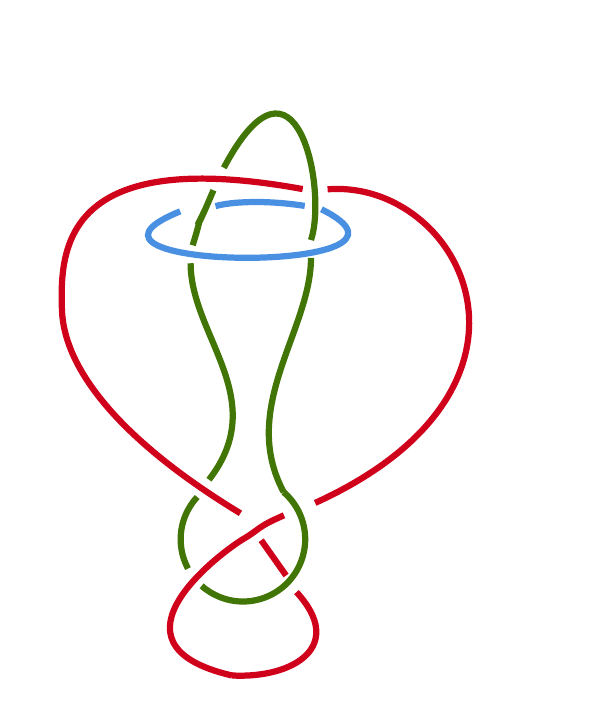
\begin{tikzpicture}[x=0.75pt,y=0.75pt,yscale=-1,xscale=1]
%uncomment if require: \path (0,300); %set diagram left start at 0, and has height of 300

%Curve Lines [id:da09943248726534226] 
\draw [color={rgb, 255:red, 208; green, 2; blue, 27 }  ,draw opacity=1 ][line width=2.25]    (343,46.68) .. controls (407,41.68) and (460,141.77) .. (337,197.77) ;
%Curve Lines [id:da6322873360352863] 
\draw [color={rgb, 255:red, 208; green, 2; blue, 27 }  ,draw opacity=1 ][line width=2.25]    (322,203.75) .. controls (309.03,209.29) and (311.19,209.93) .. (302.21,215.27) .. controls (293.23,220.61) and (231,265.75) .. (297,280.92) ;
%Curve Lines [id:da5011644671112231] 
\draw [color={rgb, 255:red, 208; green, 2; blue, 27 }  ,draw opacity=1 ][line width=2.25]    (331,46.57) .. controls (216,25.57) and (214,74.97) .. (215,104.68) .. controls (216,134.4) and (245,168.77) .. (301,202.77) ;
%Curve Lines [id:da44718777975671287] 
\draw [color={rgb, 255:red, 208; green, 2; blue, 27 }  ,draw opacity=1 ][line width=2.25]    (328,240.75) .. controls (352,266.75) and (326.73,282.41) .. (297,280.92) ;
%Shape: Arc [id:dp40054047053808206] 
\draw  [draw opacity=0][line width=2.25]  (321.85,192.58) .. controls (331.21,200.68) and (334.92,214.11) .. (330.11,226.28) .. controls (324.03,241.69) and (306.61,249.26) .. (291.19,243.17) .. controls (287.84,241.85) and (284.86,239.99) .. (282.31,237.73) -- (302.21,215.27) -- cycle ; \draw  [color={rgb, 255:red, 65; green, 117; blue, 5 }  ,draw opacity=1 ][line width=2.25]  (321.85,192.58) .. controls (331.21,200.68) and (334.92,214.11) .. (330.11,226.28) .. controls (324.03,241.69) and (306.61,249.26) .. (291.19,243.17) .. controls (287.84,241.85) and (284.86,239.99) .. (282.31,237.73) ;  
%Shape: Arc [id:dp11594177788693838] 
\draw  [draw opacity=0][line width=2.25]  (275.74,229.39) .. controls (271.75,221.9) and (270.94,212.77) .. (274.3,204.25) .. controls (275.71,200.7) and (277.71,197.56) .. (280.16,194.91) -- (302.21,215.27) -- cycle ; \draw  [color={rgb, 255:red, 65; green, 117; blue, 5 }  ,draw opacity=1 ][line width=2.25]  (275.74,229.39) .. controls (271.75,221.9) and (270.94,212.77) .. (274.3,204.25) .. controls (275.71,200.7) and (277.71,197.56) .. (280.16,194.91) ;  
%Straight Lines [id:da5976132825673692] 
\draw [color={rgb, 255:red, 208; green, 2; blue, 27 }  ,draw opacity=1 ][fill={rgb, 255:red, 208; green, 2; blue, 27 }  ,fill opacity=1 ][line width=2.25]    (311,215.75) -- (323,232.75) ;
%Curve Lines [id:da5325527173421334] 
\draw [color={rgb, 255:red, 65; green, 117; blue, 5 }  ,draw opacity=1 ][line width=2.25]    (335,79.68) .. controls (335,114.68) and (300,151.68) .. (321.85,192.58) ;
%Curve Lines [id:da2732197209903964] 
\draw [color={rgb, 255:red, 65; green, 117; blue, 5 }  ,draw opacity=1 ][line width=2.25]    (277,82.3) .. controls (277,117.3) and (316,147.68) .. (285.85,186.58) ;
%Curve Lines [id:da21608820690853647] 
\draw [color={rgb, 255:red, 65; green, 117; blue, 5 }  ,draw opacity=1 ][line width=2.25]    (278,73.65) .. controls (286,47.65) and (274,80.12) .. (288,47.12) ;
%Curve Lines [id:da1149451703987957] 
\draw [color={rgb, 255:red, 65; green, 117; blue, 5 }  ,draw opacity=1 ][line width=2.25]    (335,71.12) .. controls (343,47.12) and (328,-29.7) .. (293,36.3) ;
%Curve Lines [id:da6104443808138464] 
\draw [color={rgb, 255:red, 74; green, 144; blue, 226 }  ,draw opacity=1 ][line width=2.25]    (272,57.3) .. controls (200,86.3) and (405,88.3) .. (340,56.3) ;
%Curve Lines [id:da9503680162575591] 
\draw [color={rgb, 255:red, 74; green, 144; blue, 226 }  ,draw opacity=1 ][line width=2.25]    (289,54.8) .. controls (296,52.68) and (313,51.68) .. (332,54.68) ;




\end{tikzpicture}
  
  \caption{The knot diagram, characterising the $3^2$ link class.}
\end{figure}
\noindent
Here the blue knot corresponds to $c$ while the other two correspond to $a$ and $b$ (a,b are symmetric in the polynomial). An example of a pure state is found, as mentioned in the paper: 
$$\ket{3^2}_{abc} = \frac{1}{\sqrt{3}}\brac{\ket{000}_{abc} + \ket{111}_{abc} + \ket{001}_{abc}} $$
To check that this state indeed statistfies the link, let us calculate the density operator $\hat{\rho}_{abc}=\ket{3^2}_{abc}\bra{3^2}_{abc}$ and then check for the PPT test for each cuts. 
The density matrix obtained is: 
\begin{equation*}
    \rho_{abc}=
    \left[
    \begin{array}{cccccccc}
    0.333 & 0.333 & 0.0 & 0.0 & 0.0 & 0.0 & 0.0 & 0.333 \\
    0.333 & 0.333 & 0.0 & 0.0 & 0.0 & 0.0 & 0.0 & 0.333 \\
    0.0 & 0.0 & 0.0 & 0.0 & 0.0 & 0.0 & 0.0 & 0.0 \\
    0.0 & 0.0 & 0.0 & 0.0 & 0.0 & 0.0 & 0.0 & 0.0 \\
    0.0 & 0.0 & 0.0 & 0.0 & 0.0 & 0.0 & 0.0 & 0.0 \\
    0.0 & 0.0 & 0.0 & 0.0 & 0.0 & 0.0 & 0.0 & 0.0 \\
    0.0 & 0.0 & 0.0 & 0.0 & 0.0 & 0.0 & 0.0 & 0.0 \\
    0.333 & 0.333 & 0.0 & 0.0 & 0.0 & 0.0 & 0.0 & 0.333 \\
    \end{array}
    \right]
    \end{equation*}
    Since the variables $a$ and $b$ are symmetrix, we can choose to analyse only one of them and $c$. We then see the partial transpose with respect to $a$ and $c$. The matrices are given by:
    \begin{align*}
        \rho^{T_a}_{abc} &=
        \left[
        \begin{array}{cccccccc}
        0.333 & 0.333 & 0.0 & 0.0 & 0.0 & 0.0 & 0.0 & 0.0 \\
        0.333 & 0.333 & 0.0 & 0.0 & 0.0 & 0.0 & 0.0 & 0.0 \\
        0.0 & 0.0 & 0.0 & 0.0 & 0.0 & 0.0 & 0.0 & 0.0 \\
        0.0 & 0.0 & 0.0 & 0.0 & 0.333 & 0.333 & 0.0 & 0.0 \\
        0.0 & 0.0 & 0.0 & 0.333 & 0.0 & 0.0 & 0.0 & 0.0 \\
        0.0 & 0.0 & 0.0 & 0.333 & 0.0 & 0.0 & 0.0 & 0.0 \\
        0.0 & 0.0 & 0.0 & 0.0 & 0.0 & 0.0 & 0.0 & 0.0 \\
        0.0 & 0.0 & 0.0 & 0.0 & 0.0 & 0.0 & 0.0 & 0.333 \\
        \end{array}
        \right]\\
            \rho^{T_c}_{abc} &=
            \left[
            \begin{array}{cccccccc}
            0.333 & 0.333 & 0.0 & 0.0 & 0.0 & 0.0 & 0.0 & 0.0 \\
            0.333 & 0.333 & 0.0 & 0.0 & 0.0 & 0.0 & 0.333 & 0.333 \\
            0.0 & 0.0 & 0.0 & 0.0 & 0.0 & 0.0 & 0.0 & 0.0 \\
            0.0 & 0.0 & 0.0 & 0.0 & 0.0 & 0.0 & 0.0 & 0.0 \\
            0.0 & 0.0 & 0.0 & 0.0 & 0.0 & 0.0 & 0.0 & 0.0 \\
            0.0 & 0.0 & 0.0 & 0.0 & 0.0 & 0.0 & 0.0 & 0.0 \\
            0.0 & 0.333 & 0.0 & 0.0 & 0.0 & 0.0 & 0.0 & 0.0 \\
            0.0 & 0.333 & 0.0 & 0.0 & 0.0 & 0.0 & 0.0 & 0.333 \\
            \end{array}
            \right]
            \end{align*}
            The above matrices have eigenvalues $\lambda_a =\mathbf{\mathcolor{red}{-0.471}}, 0.0, 0.333, 0.471, 0.666$ and $\lambda_c=-0.333, 0.0, 0.127, \\0.333, 0.872 $ respectively. Since there are negative eigenvalues, we can conclude that the system exhibits \textbf{tripartite entanglement} as a whole.\\[0.3cm]
            The reduced density matrices are given by:
            \begin{align*}
                \rho_{bc} &=
                \left[
                \begin{array}{cccc}
                0.333 & 0.333 & 0.0 & 0.0 \\
                0.333 & 0.333 & 0.0 & 0.0 \\
                0.0 & 0.0 & 0.0 & 0.0 \\
                0.0 & 0.0 & 0.0 & 0.333 \\
                \end{array}
                \right]\\
                \rho_{ab} &=
                    \left[
                    \begin{array}{cccc}
                    0.666 & 0.0 & 0.0 & 0.333 \\
                    0.0 & 0.0 & 0.0 & 0.0 \\
                    0.0 & 0.0 & 0.0 & 0.0 \\
                    0.333 & 0.0 & 0.0 & 0.333 \\
                    \end{array}
                    \right]
                    \end{align*}
                   We now obtain the partial tranpose for the PPT test. We note that $\rho_{bc}^{T_b/T_c}$ is the same as that of the above matrix $\rho_{bc}$ whose eigenvalues are $0.0, 0.333, 0.666$ which are all positive. Thus, we can conclude that the system is separable. On the other hand, we obtain:
                   \begin{equation*}
                    \rho_{ab}^{T_a} =
                    \left[
                    \begin{array}{cccc}
                    0.666 & 0.0 & 0.0 & 0.0 \\
                    0.0 & 0.0 & 0.333 & 0.0 \\
                    0.0 & 0.333 & 0.0 & 0.0 \\
                    0.0 & 0.0 & 0.0 & 0.333 \\
                    \end{array}
                    \right]
                    \end{equation*}
                    The eigenvalues of this matrix are $0.333, -0.333, 0.666$, one of which is negative, thus denoting the presence of entanglement. This successfully verifies the behaviour of the link $abc+ab$. \\[0.3cm]
Using the above algorithm, we can also construct the mixed state corresponding to the link by considering the state:
$$\ket{\psi_2} = \ket{3^1}_{abc}\ket{0}_d + \ket{2^1}_{ab}\ket{0}_c\ket{1}_d$$
It is to be noted that this class has not been described in the previous works \cite{Aravind1997,Sugita2007-ko}. The density operator is then given by:
$$\hat{\rho}(a,b,c) = \frac{\Tr_d\ket{\psi_2}\bra{\psi_2}}{\sqrt{\braket{\psi_2|\psi_2}}} $$
Using numerical calculation and tracing out subsystem $d$, we found the density matrix to be:
\begin{equation*}
    \rho_{abc}=
    \left[
    \begin{array}{cccccccc}
    0.5 & 0.0 & 0.0 & 0.0 & 0.0 & 0.0 & 0.25 & 0.25 \\
    0.0 & 0.0 & 0.0 & 0.0 & 0.0 & 0.0 & 0.0 & 0.0 \\
    0.0 & 0.0 & 0.0 & 0.0 & 0.0 & 0.0 & 0.0 & 0.0 \\
    0.0 & 0.0 & 0.0 & 0.0 & 0.0 & 0.0 & 0.0 & 0.0 \\
    0.0 & 0.0 & 0.0 & 0.0 & 0.0 & 0.0 & 0.0 & 0.0 \\
    0.0 & 0.0 & 0.0 & 0.0 & 0.0 & 0.0 & 0.0 & 0.0 \\
    0.25 & 0.0 & 0.0 & 0.0 & 0.0 & 0.0 & 0.25 & 0.0 \\
    0.25 & 0.0 & 0.0 & 0.0 & 0.0 & 0.0 & 0.0 & 0.25 \\
    \end{array}
    \right]
    \end{equation*}
Let us now calculate the partial transposes for the PPT test: 
\begin{align*}
    \rho^{T_a}_{abc} &=
    \left[
    \begin{array}{cccccccc}
    0.5 & 0.0 & 0.0 & 0.0 & 0.0 & 0.0 & 0.0 & 0.0 \\
    0.0 & 0.0 & 0.0 & 0.0 & 0.0 & 0.0 & 0.0 & 0.0 \\
    0.0 & 0.0 & 0.0 & 0.0 & 0.25 & 0.0 & 0.0 & 0.0 \\
    0.0 & 0.0 & 0.0 & 0.0 & 0.25 & 0.0 & 0.0 & 0.0 \\
    0.0 & 0.0 & 0.25 & 0.25 & 0.0 & 0.0 & 0.0 & 0.0 \\
    0.0 & 0.0 & 0.0 & 0.0 & 0.0 & 0.0 & 0.0 & 0.0 \\
    0.0 & 0.0 & 0.0 & 0.0 & 0.0 & 0.0 & 0.25 & 0.0 \\
    0.0 & 0.0 & 0.0 & 0.0 & 0.0 & 0.0 & 0.0 & 0.25 \\
    \end{array}
    \right]
    \\
    \rho^{T_b}_{abc} &=
    \left[
    \begin{array}{cccccccc}
    0.5 & 0.0 & 0.0 & 0.0 & 0.0 & 0.0 & 0.0 & 0.0 \\
    0.0 & 0.0 & 0.0 & 0.0 & 0.0 & 0.0 & 0.0 & 0.0 \\
    0.0 & 0.0 & 0.0 & 0.0 & 0.25 & 0.25 & 0.0 & 0.0 \\
    0.0 & 0.0 & 0.0 & 0.0 & 0.0 & 0.0 & 0.0 & 0.0 \\
    0.0 & 0.0 & 0.25 & 0.0 & 0.0 & 0.0 & 0.0 & 0.0 \\
    0.0 & 0.0 & 0.25 & 0.0 & 0.0 & 0.0 & 0.0 & 0.0 \\
    0.0 & 0.0 & 0.0 & 0.0 & 0.0 & 0.0 & 0.25 & 0.0 \\
    0.0 & 0.0 & 0.0 & 0.0 & 0.0 & 0.0 & 0.0 & 0.25 \\
    \end{array}
    \right]
    \\
    \rho^{T_c}_{abc} &=
    \left[
    \begin{array}{cccccccc}
    0.5 & 0.0 & 0.0 & 0.0 & 0.0 & 0.0 & 0.25 & 0.0 \\
    0.0 & 0.0 & 0.0 & 0.0 & 0.0 & 0.0 & 0.25 & 0.0 \\
    0.0 & 0.0 & 0.0 & 0.0 & 0.0 & 0.0 & 0.0 & 0.0 \\
    0.0 & 0.0 & 0.0 & 0.0 & 0.0 & 0.0 & 0.0 & 0.0 \\
    0.0 & 0.0 & 0.0 & 0.0 & 0.0 & 0.0 & 0.0 & 0.0 \\
    0.0 & 0.0 & 0.0 & 0.0 & 0.0 & 0.0 & 0.0 & 0.0 \\
    0.25 & 0.25 & 0.0 & 0.0 & 0.0 & 0.0 & 0.25 & 0.0 \\
    0.0 & 0.0 & 0.0 & 0.0 & 0.0 & 0.0 & 0.0 & 0.25 \\
    \end{array}
    \right]
    \end{align*}
    
    The set of eigenvalues for the above matrices are:
    \begin{itemize}
        \item $ \lambda_a = \mathbf{\mathcolor{red}{-0.354}}, 0.0, 0.0, 0.0, 0.25, 0.25, 0.354, 0.5$
        \item $ \lambda_b = \mathbf{\mathcolor{red}{-0.354}}, 0.0, 0.0, 0.0, 0.25, 0.25, 0.354, 0.5$
        \item $ \lambda_c = \mathbf{\mathcolor{red}{-0.183}}, 0.0, 0.0, 0.0, 0.0, 0.25, 0.25, 0.683$
    \end{itemize}
Each of the above matrices have atleast one negative eigenvalues, thus denoting the presence of entanglement in the system as a whole. Let us now analyse the reduced density matrices and their PPT matrices which corresponds to the act of `cutting a link': 
\begin{align*}
    \rho_{bc} &=
    \left[
    \begin{array}{cccc}
    0.5 & 0.0 & 0.0 & 0.0 \\
    0.0 & 0.0 & 0.0 & 0.0 \\
    0.0 & 0.0 & 0.25 & 0.0 \\
    0.0 & 0.0 & 0.0 & 0.25 \\
    \end{array}
    \right] \quad \rho_{bc}^{T_b} = \left[
        \begin{array}{cccc}
        0.5 & 0.0 & 0.0 & 0.0 \\
        0.0 & 0.0 & 0.0 & 0.0 \\
        0.0 & 0.0 & 0.25 & 0.0 \\
        0.0 & 0.0 & 0.0 & 0.25 \\
        \end{array}
        \right]
    \\
    \rho_{ac} &=
    \left[
    \begin{array}{cccc}
    0.5 & 0.0 & 0.0 & 0.0 \\
    0.0 & 0.0 & 0.0 & 0.0 \\
    0.0 & 0.0 & 0.25 & 0.0 \\
    0.0 & 0.0 & 0.0 & 0.25 \\
    \end{array}
    \right] \quad \rho_{ac}^{T_a} =\left[
        \begin{array}{cccc}
        0.5 & 0.0 & 0.0 & 0.0 \\
        0.0 & 0.0 & 0.0 & 0.0 \\
        0.0 & 0.0 & 0.25 & 0.0 \\
        0.0 & 0.0 & 0.0 & 0.25 \\
        \end{array}
        \right]
    \\
    \rho_{ab} &=
    \left[
    \begin{array}{cccc}
    0.5 & 0.0 & 0.0 & 0.25 \\
    0.0 & 0.0 & 0.0 & 0.0 \\
    0.0 & 0.0 & 0.0 & 0.0 \\
    0.25 & 0.0 & 0.0 & 0.5 \\
    \end{array}
    \right] \quad \rho_{ab}^{T_a} = \left[
        \begin{array}{cccc}
        0.5 & 0.0 & 0.0 & 0.0 \\
        0.0 & 0.0 & 0.25 & 0.0 \\
        0.0 & 0.25 & 0.0 & 0.0 \\
        0.0 & 0.0 & 0.0 & 0.5 \\
        \end{array}
        \right]
    \end{align*}
    
    The set of eigenvalues for the above matrices are:
    \begin{itemize}
        \item $0.0, 0.25, 0.25, 0.5 \longrightarrow$ no eigenvalue is negative, thus cutting $a$ separates the systems $b$ and $c$.        
        \item $0.0, 0.25, 0.25, 0.5 \longrightarrow$ no eigenvalue is negative, thus cutting $b$ separates the systems $a$ and $c$.        
       \item $ \mathbf{\mathcolor{red}{-0.25},} 0.25, 0.5, 0.5 \longrightarrow$ one eigenvalue is negative, thus on cutting $c$, the systems $a$ and $b$ remain entangled.
    \end{itemize}
    This faithfully reproduces the behaviour of the link $abc+ab$ and thus, the state characterises the link.\begin{figure}[H]
        \centering
        \scalebox{0.8}{ 

\tikzset{every picture/.style={line width=0.75pt}} %set default line width to 0.75pt        

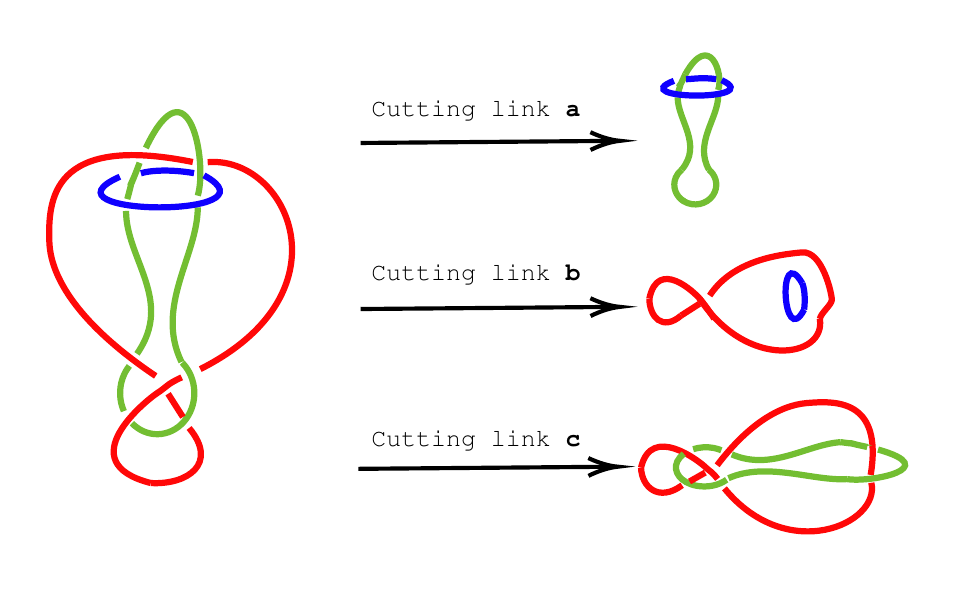
\begin{tikzpicture}[x=0.75pt,y=0.75pt,yscale=-1,xscale=1]
%uncomment if require: \path (0,300); %set diagram left start at 0, and has height of 300

%Curve Lines [id:da12875223491219945] 
\draw [color={rgb, 255:red, 255; green, 8; blue, 8 }  ,draw opacity=1 ][line width=2.25]    (167.36,66.26) .. controls (205.5,62.96) and (237.09,129.01) .. (163.78,165.96) ;
%Curve Lines [id:da8552594726616213] 
\draw [color={rgb, 255:red, 255; green, 8; blue, 8 }  ,draw opacity=1 ][line width=2.25]    (154.84,169.91) .. controls (147.12,173.57) and (148.4,173.99) .. (143.05,177.51) .. controls (137.7,181.03) and (100.61,210.83) .. (139.94,220.84) ;
%Curve Lines [id:da009148374133189585] 
\draw [color={rgb, 255:red, 255; green, 8; blue, 8 }  ,draw opacity=1 ][line width=2.25]    (160.21,66.18) .. controls (91.67,52.32) and (90.48,84.92) .. (91.08,104.53) .. controls (91.67,124.14) and (108.96,146.82) .. (142.33,169.26) ;
%Curve Lines [id:da6982542275996216] 
\draw [color={rgb, 255:red, 255; green, 8; blue, 8 }  ,draw opacity=1 ][line width=2.25]    (158.42,194.33) .. controls (172.72,211.49) and (157.66,221.82) .. (139.94,220.84) ;
%Shape: Arc [id:dp5661257343878181] 
\draw  [draw opacity=0][line width=2.25]  (155.06,162.84) .. controls (160.41,168.22) and (162.49,176.9) .. (159.68,184.78) .. controls (156.05,194.95) and (145.67,199.94) .. (136.48,195.93) .. controls (134.35,194.99) and (132.46,193.65) .. (130.87,192.02) -- (143.05,177.51) -- cycle ; \draw  [color={rgb, 255:red, 115; green, 190; blue, 50 }  ,draw opacity=1 ][line width=2.25]  (155.06,162.84) .. controls (160.41,168.22) and (162.49,176.9) .. (159.68,184.78) .. controls (156.05,194.95) and (145.67,199.94) .. (136.48,195.93) .. controls (134.35,194.99) and (132.46,193.65) .. (130.87,192.02) ;  
%Shape: Arc [id:dp8791859009639712] 
\draw  [draw opacity=0][line width=2.25]  (126.98,186.2) .. controls (124.86,181.38) and (124.5,175.63) .. (126.42,170.24) .. controls (127.2,168.05) and (128.3,166.1) .. (129.63,164.43) -- (143.05,177.51) -- cycle ; \draw  [color={rgb, 255:red, 115; green, 190; blue, 50 }  ,draw opacity=1 ][line width=2.25]  (126.98,186.2) .. controls (124.86,181.38) and (124.5,175.63) .. (126.42,170.24) .. controls (127.2,168.05) and (128.3,166.1) .. (129.63,164.43) ;  
%Straight Lines [id:da2087504851234686] 
\draw [color={rgb, 255:red, 255; green, 8; blue, 8 }  ,draw opacity=1 ][fill={rgb, 255:red, 208; green, 2; blue, 27 }  ,fill opacity=1 ][line width=2.25]    (148.29,177.83) -- (155.44,189.05) ;
%Curve Lines [id:da20849263880719082] 
\draw [color={rgb, 255:red, 115; green, 190; blue, 50 }  ,draw opacity=1 ][line width=2.25]    (162.59,88.03) .. controls (162.59,111.13) and (141.73,135.55) .. (154.75,162.54) ;
%Curve Lines [id:da0588954229632106] 
\draw [color={rgb, 255:red, 115; green, 190; blue, 50 }  ,draw opacity=1 ][line width=2.25]    (128.03,89.76) .. controls (128.03,112.86) and (151.27,132.91) .. (133.3,158.58) ;
%Curve Lines [id:da860090698559123] 
\draw [color={rgb, 255:red, 115; green, 190; blue, 50 }  ,draw opacity=1 ][line width=2.25]    (128.62,84.05) .. controls (133.39,66.89) and (126.24,88.32) .. (134.58,66.54) ;
%Curve Lines [id:da413135274152026] 
\draw [color={rgb, 255:red, 115; green, 190; blue, 50 }  ,draw opacity=1 ][line width=2.25]    (162.59,82.38) .. controls (167.36,66.54) and (158.42,15.85) .. (137.56,59.4) ;
%Curve Lines [id:da14507504444650798] 
\draw [color={rgb, 255:red, 15; green, 0; blue, 255 }  ,draw opacity=1 ][line width=2.25]    (125.05,73.26) .. controls (82.14,92.4) and (204.31,93.72) .. (165.57,72.6) ;
%Curve Lines [id:da15354691086785033] 
\draw [color={rgb, 255:red, 15; green, 0; blue, 255 }  ,draw opacity=1 ][line width=2.25]    (135.18,71.61) .. controls (139.35,70.22) and (149.48,69.56) .. (160.8,71.54) ;
%Straight Lines [id:da3134846016152506] 
\draw [line width=1.5]    (241,57) -- (284.98,56.64) -- (363,55.99) ;
\draw [shift={(366,55.97)}, rotate = 179.53] [color={rgb, 255:red, 0; green, 0; blue, 0 }  ][line width=1.5]    (14.21,-4.28) .. controls (9.04,-1.82) and (4.3,-0.39) .. (0,0) .. controls (4.3,0.39) and (9.04,1.82) .. (14.21,4.28)   ;
%Straight Lines [id:da9569788198448126] 
\draw [line width=1.5]    (241,137) -- (284.98,136.64) -- (363,135.99) ;
\draw [shift={(366,135.97)}, rotate = 179.53] [color={rgb, 255:red, 0; green, 0; blue, 0 }  ][line width=1.5]    (14.21,-4.28) .. controls (9.04,-1.82) and (4.3,-0.39) .. (0,0) .. controls (4.3,0.39) and (9.04,1.82) .. (14.21,4.28)   ;
%Straight Lines [id:da08772413911010224] 
\draw [line width=1.5]    (240,214) -- (283.98,213.64) -- (362,212.99) ;
\draw [shift={(365,212.97)}, rotate = 179.53] [color={rgb, 255:red, 0; green, 0; blue, 0 }  ][line width=1.5]    (14.21,-4.28) .. controls (9.04,-1.82) and (4.3,-0.39) .. (0,0) .. controls (4.3,0.39) and (9.04,1.82) .. (14.21,4.28)   ;
%Shape: Arc [id:dp531278752687114] 
\draw  [draw opacity=0][line width=2.25]  (408.8,69.84) .. controls (412.03,72.39) and (413.33,76.7) .. (411.69,80.6) .. controls (409.64,85.48) and (403.77,87.87) .. (398.58,85.95) .. controls (397.5,85.55) and (396.53,84.99) .. (395.7,84.31) -- (402.29,77.11) -- cycle ; \draw  [color={rgb, 255:red, 115; green, 190; blue, 50 }  ,draw opacity=1 ][line width=2.25]  (408.8,69.84) .. controls (412.03,72.39) and (413.33,76.7) .. (411.69,80.6) .. controls (409.64,85.48) and (403.77,87.87) .. (398.58,85.95) .. controls (397.5,85.55) and (396.53,84.99) .. (395.7,84.31) ;  
%Shape: Arc [id:dp019593257892404514] 
\draw  [draw opacity=0][line width=2.25]  (396.98,85.2) .. controls (392.89,82.83) and (391.06,77.97) .. (392.89,73.62) .. controls (393.53,72.09) and (394.55,70.81) .. (395.8,69.82) -- (402.29,77.11) -- cycle ; \draw  [color={rgb, 255:red, 115; green, 190; blue, 50 }  ,draw opacity=1 ][line width=2.25]  (396.98,85.2) .. controls (392.89,82.83) and (391.06,77.97) .. (392.89,73.62) .. controls (393.53,72.09) and (394.55,70.81) .. (395.8,69.82) ;  
%Curve Lines [id:da49715416371135246] 
\draw [color={rgb, 255:red, 115; green, 190; blue, 50 }  ,draw opacity=1 ][line width=2.25]    (413.34,34.17) .. controls (413.34,45.25) and (401.55,56.97) .. (408.91,69.92) ;
%Curve Lines [id:da7628262692824233] 
\draw [color={rgb, 255:red, 115; green, 190; blue, 50 }  ,draw opacity=1 ][line width=2.25]    (393.8,35) .. controls (393.8,46.08) and (405.96,57.5) .. (395.8,69.82) ;
%Curve Lines [id:da15776170677437595] 
\draw [color={rgb, 255:red, 115; green, 190; blue, 50 }  ,draw opacity=1 ][line width=2.25]    (394.14,32.26) .. controls (396.83,24.02) and (392.79,34.3) .. (397.5,23.85) ;
%Curve Lines [id:da6639875574644403] 
\draw [color={rgb, 255:red, 115; green, 190; blue, 50 }  ,draw opacity=1 ][line width=2.25]    (413.34,31.45) .. controls (416.03,23.85) and (409.29,2.95) .. (397.5,23.85) ;
%Curve Lines [id:da3889899808295765] 
\draw [color={rgb, 255:red, 15; green, 0; blue, 255 }  ,draw opacity=1 ][line width=2.25]    (392,27.07) .. controls (367.75,36.25) and (436.91,36.9) .. (415.02,26.76) ;
%Curve Lines [id:da3769808426781921] 
\draw [color={rgb, 255:red, 15; green, 0; blue, 255 }  ,draw opacity=1 ][line width=2.25]    (397.84,26.29) .. controls (401,26.17) and (405.92,25.3) .. (412.32,26.25) ;
%Curve Lines [id:da04168948675118911] 
\draw [color={rgb, 255:red, 255; green, 8; blue, 8 }  ,draw opacity=1 ][line width=2.25]    (462.29,141.79) .. controls (465.41,160.56) and (427.29,166.8) .. (404.3,131.87) ;
%Curve Lines [id:da18467694946613922] 
\draw [color={rgb, 255:red, 255; green, 8; blue, 8 }  ,draw opacity=1 ][line width=2.25]    (411.41,141.71) .. controls (409.12,138.02) and (406.44,134.39) .. (404.3,131.87) .. controls (402.17,129.35) and (384.38,112.11) .. (380.16,131.97) ;
%Curve Lines [id:da8722190077480936] 
\draw [color={rgb, 255:red, 255; green, 8; blue, 8 }  ,draw opacity=1 ][line width=2.25]    (462.29,141.79) .. controls (462.73,138.97) and (467.93,135.03) .. (468.07,132.62) .. controls (468.21,130.21) and (463.62,108.77) .. (453.65,109.72) .. controls (443.67,110.68) and (420.55,113.15) .. (409.22,130.54) ;
%Curve Lines [id:da12756001604786704] 
\draw [color={rgb, 255:red, 255; green, 8; blue, 8 }  ,draw opacity=1 ][line width=2.25]    (395.49,140.13) .. controls (386.45,147.86) and (380.21,140.79) .. (380.16,131.97) ;
%Straight Lines [id:da6083498463348601] 
\draw [color={rgb, 255:red, 255; green, 8; blue, 8 }  ,draw opacity=1 ][fill={rgb, 255:red, 208; green, 2; blue, 27 }  ,fill opacity=1 ][line width=2.25]    (404.3,134.48) -- (395.49,140.13) ;
%Curve Lines [id:da2675295109724416] 
\draw [color={rgb, 255:red, 15; green, 0; blue, 255 }  ,draw opacity=1 ][line width=2.25]    (453.82,124.58) .. controls (441.75,104.04) and (444.32,157.27) .. (454.73,137.27) ;
%Curve Lines [id:da34703185132477266] 
\draw [color={rgb, 255:red, 15; green, 0; blue, 255 }  ,draw opacity=1 ][line width=2.25]    (453.82,124.58) .. controls (454.74,126.59) and (455.45,131.59) .. (454.73,137.27) ;
%Curve Lines [id:da3428791500345205] 
\draw [color={rgb, 255:red, 255; green, 8; blue, 8 }  ,draw opacity=1 ][line width=2.25]    (487.13,220.7) .. controls (491.56,240.62) and (446.52,260.29) .. (416.33,223.42) ;
%Curve Lines [id:da09145183935237511] 
\draw [color={rgb, 255:red, 255; green, 8; blue, 8 }  ,draw opacity=1 ][line width=2.25]    (413.04,218.9) .. controls (410.03,215) and (409.8,215.7) .. (407.01,213.04) .. controls (404.23,210.39) and (381.1,192.25) .. (376.16,213.41) ;
%Curve Lines [id:da9002899251329601] 
\draw [color={rgb, 255:red, 255; green, 8; blue, 8 }  ,draw opacity=1 ][line width=2.25]    (486.79,216.94) .. controls (492.85,180.23) and (469.7,181.11) .. (455.84,182.33) .. controls (441.99,183.54) and (426.88,193.69) .. (412.82,212.28) ;
%Curve Lines [id:da18604085337754517] 
\draw [color={rgb, 255:red, 255; green, 8; blue, 8 }  ,draw opacity=1 ][line width=2.25]    (395.95,221.91) .. controls (384.58,230.23) and (376.44,222.78) .. (376.16,213.41) ;
%Shape: Arc [id:dp51615588916968] 
\draw  [draw opacity=0][line width=2.25]  (417.39,219.23) .. controls (413.81,221.92) and (408.17,223.17) .. (402.78,222.13) .. controls (395.38,220.69) and (391.27,215.46) .. (393.61,210.44) .. controls (394.27,209.03) and (395.37,207.79) .. (396.77,206.76) -- (407.01,213.04) -- cycle ; \draw  [color={rgb, 255:red, 115; green, 190; blue, 50 }  ,draw opacity=1 ][line width=2.25]  (417.39,219.23) .. controls (413.81,221.92) and (408.17,223.17) .. (402.78,222.13) .. controls (395.38,220.69) and (391.27,215.46) .. (393.61,210.44) .. controls (394.27,209.03) and (395.37,207.79) .. (396.77,206.76) ;  
%Shape: Arc [id:dp5020648069456706] 
\draw  [draw opacity=0][line width=2.25]  (401.27,204.53) .. controls (404.3,203.56) and (407.83,203.29) .. (411.25,203.96) .. controls (412.56,204.21) and (413.76,204.59) .. (414.85,205.06) -- (407.01,213.04) -- cycle ; \draw  [color={rgb, 255:red, 115; green, 190; blue, 50 }  ,draw opacity=1 ][line width=2.25]  (401.27,204.53) .. controls (404.3,203.56) and (407.83,203.29) .. (411.25,203.96) .. controls (412.56,204.21) and (413.76,204.59) .. (414.85,205.06) ;  
%Straight Lines [id:da5581942332188228] 
\draw [color={rgb, 255:red, 255; green, 8; blue, 8 }  ,draw opacity=1 ][fill={rgb, 255:red, 208; green, 2; blue, 27 }  ,fill opacity=1 ][line width=2.25]    (407.08,215.82) -- (399.52,220.1) ;
%Curve Lines [id:da9488913221978837] 
\draw [color={rgb, 255:red, 115; green, 190; blue, 50 }  ,draw opacity=1 ][line width=2.25]    (475.45,218.94) .. controls (459.09,220) and (436.66,210.41) .. (418.26,218.51) ;
%Curve Lines [id:da7482325423285066] 
\draw [color={rgb, 255:red, 115; green, 190; blue, 50 }  ,draw opacity=1 ][line width=2.25]    (472.4,201.14) .. controls (456.05,202.2) and (439.05,215.31) .. (419.89,207.04) ;
%Curve Lines [id:da967631793204382] 
\draw [color={rgb, 255:red, 115; green, 190; blue, 50 }  ,draw opacity=1 ][line width=2.25]    (472.4,201.14) .. controls (484.82,202.86) and (469.25,200.08) .. (485.13,203.47) ;
%Curve Lines [id:da7962523321097766] 
\draw [color={rgb, 255:red, 115; green, 190; blue, 50 }  ,draw opacity=1 ][line width=2.25]    (475.45,218.94) .. controls (486.93,220.72) and (522.34,213.67) .. (490.35,204.71) ;

% Text Node
\draw (245,35) node [anchor=north west][inner sep=0.75pt]  [font=\small] [align=left] {{\fontfamily{pcr}\selectfont Cutting link \textbf{a}}};
% Text Node
\draw (245,114) node [anchor=north west][inner sep=0.75pt]  [font=\small] [align=left] {{\fontfamily{pcr}\selectfont Cutting link \textbf{b}}};
% Text Node
\draw (245,194) node [anchor=north west][inner sep=0.75pt]  [font=\small] [align=left] {{\fontfamily{pcr}\selectfont Cutting link \textbf{c}}};


\end{tikzpicture}
}
        \caption{Possible link cuts for the $3^2$ link class. Two cuts lead to complete separability while other cut lead to different entangled configuration.}
    \end{figure}
    \noindent
\textbf{\large \texttt{3\textsuperscript{3}} Link Class} \\[0.3cm]
We now analyse the link class given by $P_3(a,b,c) = ab+ac$. The link diagram is given by:
\begin{figure}[H]
    \centering
  

\tikzset{every picture/.style={line width=0.75pt}} %set default line width to 0.75pt        

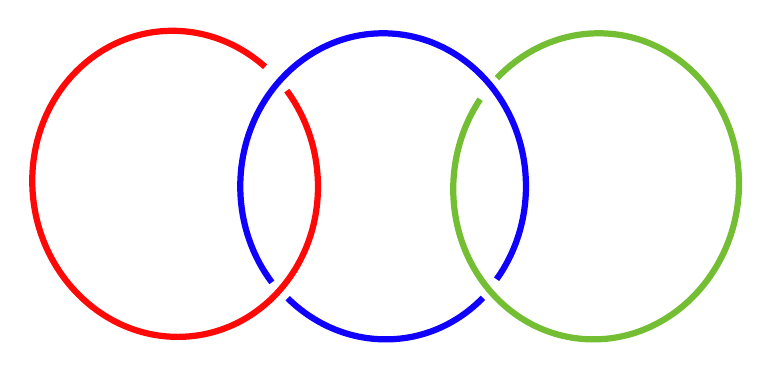
\begin{tikzpicture}[x=0.75pt,y=0.75pt,yscale=-1,xscale=1]
%uncomment if require: \path (0,300); %set diagram left start at 0, and has height of 300

%Shape: Arc [id:dp45545170377512756] 
\draw  [draw opacity=0][line width=2.25]  (234.67,185.2) .. controls (225.14,172.55) and (219.44,156.46) .. (219.44,138.93) .. controls (219.44,98.21) and (250.25,65.2) .. (288.26,65.2) .. controls (326.26,65.2) and (357.08,98.21) .. (357.08,138.93) .. controls (357.08,155.77) and (351.81,171.29) .. (342.94,183.71) -- (288.26,138.93) -- cycle ; \draw  [color={rgb, 255:red, 15; green, 0; blue, 255 }  ,draw opacity=1 ][line width=2.25]  (234.67,185.2) .. controls (225.14,172.55) and (219.44,156.46) .. (219.44,138.93) .. controls (219.44,98.21) and (250.25,65.2) .. (288.26,65.2) .. controls (326.26,65.2) and (357.08,98.21) .. (357.08,138.93) .. controls (357.08,155.77) and (351.81,171.29) .. (342.94,183.71) ;  
%Shape: Arc [id:dp43179396468586795] 
\draw  [draw opacity=0][line width=2.25]  (336.36,192.63) .. controls (324.26,205.05) and (307.81,212.67) .. (289.56,212.67) .. controls (271.41,212.67) and (254.78,205.14) .. (242.27,192.85) -- (288.26,138.93) -- cycle ; \draw  [color={rgb, 255:red, 15; green, 0; blue, 255 }  ,draw opacity=1 ][line width=2.25]  (336.36,192.63) .. controls (324.26,205.05) and (307.81,212.67) .. (289.56,212.67) .. controls (271.41,212.67) and (254.78,205.14) .. (242.27,192.85) ;  
%Shape: Arc [id:dp1272193908857524] 
\draw  [draw opacity=0][line width=2.25]  (241.85,92.84) .. controls (250.99,105.27) and (256.56,120.84) .. (256.86,137.73) .. controls (257.58,178.46) and (227.35,211.47) .. (189.34,211.47) .. controls (151.34,211.47) and (119.94,178.46) .. (119.23,137.73) .. controls (118.51,97.01) and (148.74,64) .. (186.74,64) .. controls (203.64,64) and (219.23,70.53) .. (231.4,81.35) -- (188.04,137.73) -- cycle ; \draw  [color={rgb, 255:red, 255; green, 8; blue, 8 }  ,draw opacity=1 ][line width=2.25]  (241.85,92.84) .. controls (250.99,105.27) and (256.56,120.84) .. (256.86,137.73) .. controls (257.58,178.46) and (227.35,211.47) .. (189.34,211.47) .. controls (151.34,211.47) and (119.94,178.46) .. (119.23,137.73) .. controls (118.51,97.01) and (148.74,64) .. (186.74,64) .. controls (203.64,64) and (219.23,70.53) .. (231.4,81.35) ;  
%Shape: Arc [id:dp33396414047455336] 
\draw  [draw opacity=0][line width=2.25]  (335.01,96.98) .. controls (327.1,108.89) and (322.33,123.35) .. (322.06,138.93) .. controls (321.34,179.65) and (351.57,212.67) .. (389.58,212.67) .. controls (427.59,212.67) and (458.99,179.65) .. (459.71,138.93) .. controls (460.43,98.21) and (430.19,65.2) .. (392.18,65.2) .. controls (373.16,65.2) and (355.8,73.46) .. (343.11,86.82) -- (390.88,138.93) -- cycle ; \draw  [color={rgb, 255:red, 115; green, 190; blue, 50 }  ,draw opacity=1 ][line width=2.25]  (335.01,96.98) .. controls (327.1,108.89) and (322.33,123.35) .. (322.06,138.93) .. controls (321.34,179.65) and (351.57,212.67) .. (389.58,212.67) .. controls (427.59,212.67) and (458.99,179.65) .. (459.71,138.93) .. controls (460.43,98.21) and (430.19,65.2) .. (392.18,65.2) .. controls (373.16,65.2) and (355.8,73.46) .. (343.11,86.82) ;  




\end{tikzpicture}
  
  \caption{The knot diagram, characterising the $3^3$ link class.}
\end{figure}
\noindent
We can see that the knot polynomial is symmetric in $b$ and $c$. Thus, if we cut either $b$ or $c$, the other will remain entangled with $a$ but complete separation results from cutting $a$. This case has already been discussed in section \ref{link_from_state} and a pure state has been obtained. The mixed state can be obtained using the state:
$$\ket{\psi_3} = \ket{2^1}_{ab}\ket{0}_c\ket{0}_d + \ket{2^1}_{ac}\ket{1}_b\ket{1}_d  $$ 
The density matrix obtained for the system is: 
\begin{equation*}
    \rho_{abc}=
    \left[
    \begin{array}{cccccccc}
    0.25 & 0.0 & 0.0 & 0.0 & 0.0 & 0.0 & 0.25 & 0.0 \\
    0.0 & 0.0 & 0.0 & 0.0 & 0.0 & 0.0 & 0.0 & 0.0 \\
    0.0 & 0.0 & 0.25 & 0.0 & 0.0 & 0.0 & 0.0 & 0.25 \\
    0.0 & 0.0 & 0.0 & 0.0 & 0.0 & 0.0 & 0.0 & 0.0 \\
    0.0 & 0.0 & 0.0 & 0.0 & 0.0 & 0.0 & 0.0 & 0.0 \\
    0.0 & 0.0 & 0.0 & 0.0 & 0.0 & 0.0 & 0.0 & 0.0 \\
    0.25 & 0.0 & 0.0 & 0.0 & 0.0 & 0.0 & 0.25 & 0.0 \\
    0.0 & 0.0 & 0.25 & 0.0 & 0.0 & 0.0 & 0.0 & 0.25 \\
    \end{array}
    \right]
    \end{equation*}
    Let us calculate the partial transposes for the PPT test: 
    \begin{align*}
        \rho^{T_a}_{abc} &=
        \left[
        \begin{array}{cccccccc}
        0.25 & 0.0 & 0.0 & 0.0 & 0.0 & 0.0 & 0.0 & 0.0 \\
        0.0 & 0.0 & 0.0 & 0.0 & 0.0 & 0.0 & 0.0 & 0.0 \\
        0.0 & 0.0 & 0.25 & 0.0 & 0.25 & 0.0 & 0.0 & 0.0 \\
        0.0 & 0.0 & 0.0 & 0.0 & 0.0 & 0.0 & 0.25 & 0.0 \\
        0.0 & 0.0 & 0.25 & 0.0 & 0.0 & 0.0 & 0.0 & 0.0 \\
        0.0 & 0.0 & 0.0 & 0.0 & 0.0 & 0.0 & 0.0 & 0.0 \\
        0.0 & 0.0 & 0.0 & 0.25 & 0.0 & 0.0 & 0.25 & 0.0 \\
        0.0 & 0.0 & 0.0 & 0.0 & 0.0 & 0.0 & 0.0 & 0.25 \\
        \end{array}
        \right]\\  \rho^{T_b}_{abc} &=
        \left[
        \begin{array}{cccccccc}
        0.25 & 0.0 & 0.0 & 0.0 & 0.0 & 0.0 & 0.0 & 0.0 \\
        0.0 & 0.0 & 0.0 & 0.0 & 0.0 & 0.0 & 0.0 & 0.0 \\
        0.0 & 0.0 & 0.25 & 0.0 & 0.25 & 0.0 & 0.0 & 0.25 \\
        0.0 & 0.0 & 0.0 & 0.0 & 0.0 & 0.0 & 0.0 & 0.0 \\
        0.0 & 0.0 & 0.25 & 0.0 & 0.0 & 0.0 & 0.0 & 0.0 \\
        0.0 & 0.0 & 0.0 & 0.0 & 0.0 & 0.0 & 0.0 & 0.0 \\
        0.0 & 0.0 & 0.0 & 0.0 & 0.0 & 0.0 & 0.25 & 0.0 \\
        0.0 & 0.0 & 0.25 & 0.0 & 0.0 & 0.0 & 0.0 & 0.25 \\
        \end{array}
        \right]\\  \rho^{T_c}_{abc} &=
        \left[
        \begin{array}{cccccccc}
        0.25 & 0.0 & 0.0 & 0.0 & 0.0 & 0.0 & 0.25 & 0.0 \\
        0.0 & 0.0 & 0.0 & 0.0 & 0.0 & 0.0 & 0.0 & 0.0 \\
        0.0 & 0.0 & 0.25 & 0.0 & 0.0 & 0.0 & 0.0 & 0.0 \\
        0.0 & 0.0 & 0.0 & 0.0 & 0.0 & 0.0 & 0.25 & 0.0 \\
        0.0 & 0.0 & 0.0 & 0.0 & 0.0 & 0.0 & 0.0 & 0.0 \\
        0.0 & 0.0 & 0.0 & 0.0 & 0.0 & 0.0 & 0.0 & 0.0 \\
        0.25 & 0.0 & 0.0 & 0.25 & 0.0 & 0.0 & 0.25 & 0.0 \\
        0.0 & 0.0 & 0.0 & 0.0 & 0.0 & 0.0 & 0.0 & 0.25 \\
        \end{array}
        \right]
        \end{align*}
        The set of eigenvalues obtained for the above matrices are: 
        \begin{itemize}
            \item $\lambda_a =\mathbf{\mathcolor{red}{-0.155}}, \mathbf{\mathcolor{red}{-0.155}}, 0.0, 0.0, 0.25, 0.25, 0.405, 0.405$
            \item $\lambda_b = \mathbf{\mathcolor{red}{-0.2}, }0.0, 0.0, 0.0, 0.139, 0.25, 0.25, 0.562$
            \item $\lambda_c = \mathbf{\mathcolor{red}{-0.2}, }0.0, 0.0, 0.0, 0.139, 0.25, 0.25, 0.562$
        \end{itemize}
        Since atleast one of the eigenvalues is negative for each matrix, we can conclude that the system exhibits \textbf{tripartite entanglement} as a whole. Let us now consider the reduced systems. We obtain the density matrices and their PPT matrices for the reduced system as:
        \begin{align*}
            \rho_{bc} &= 
            \left[
            \begin{array}{cccc}
            0.25 & 0.0 & 0.0 & 0.0 \\
            0.0 & 0.0 & 0.0 & 0.0 \\
            0.0 & 0.0 & 0.5 & 0.0 \\
            0.0 & 0.0 & 0.0 & 0.25 \\
            \end{array}
            \right] \quad \rho_{bc}^{T_b} = \left[
                \begin{array}{cccc}
                0.25 & 0.0 & 0.0 & 0.0 \\
                0.0 & 0.0 & 0.0 & 0.0 \\
                0.0 & 0.0 & 0.5 & 0.0 \\
                0.0 & 0.0 & 0.0 & 0.25 \\
                \end{array}
                \right]\\
            \rho_{ac} &=
            \left[
            \begin{array}{cccc}
            0.5 & 0.0 & 0.0 & 0.25 \\
            0.0 & 0.0 & 0.0 & 0.0 \\
            0.0 & 0.0 & 0.25 & 0.0 \\
            0.25 & 0.0 & 0.0 & 0.25 \\
            \end{array}
            \right] \quad \rho_{ac}^{T_a} = \left[
                \begin{array}{cccc}
                0.5 & 0.0 & 0.0 & 0.0 \\
                0.0 & 0.0 & 0.25 & 0.0 \\
                0.0 & 0.25 & 0.25 & 0.0 \\
                0.0 & 0.0 & 0.0 & 0.25 \\
                \end{array}
                \right]\\
            \rho_{ab} &=
            \left[
            \begin{array}{cccc}
            0.25 & 0.0 & 0.0 & 0.25 \\
            0.0 & 0.25 & 0.0 & 0.0 \\
            0.0 & 0.0 & 0.0 & 0.0 \\
            0.25 & 0.0 & 0.0 & 0.5 \\
            \end{array}
            \right]\quad \rho_{ab}^{T_a} = \left[
                \begin{array}{cccc}
                0.25 & 0.0 & 0.0 & 0.0 \\
                0.0 & 0.25 & 0.25 & 0.0 \\
                0.0 & 0.25 & 0.0 & 0.0 \\
                0.0 & 0.0 & 0.0 & 0.5 \\
                \end{array}
                \right]
            \end{align*}
            The set of eigenvalues obtained for the above matrices are:
            \begin{itemize}
                \item $0.0, 0.25, 0.25, 0.5 \longrightarrow$ no negative eigenvalues, so cutting $a$ makes the system separable.        
                \item $\mathbf{\mathcolor{red}{-0.155}}, 0.25, 0.405, 0.5$ $\longrightarrow$ negative eigenvalue, so on cutting $b$, system $a$ and $c$ remain entangled.
                \item $\mathbf{\mathcolor{red}{-0.155}}, 0.25, 0.405, 0.5$ $\longrightarrow$ negative eigenvalue, so on cutting $c$  system $a$ and $b$ remain entangled.
            \end{itemize}
            This is consistent with the link properties and hence the mixed state obtained is indeed characterises the link. 
            \begin{figure}[H]
                \centering
                \scalebox{0.8}{ 

\tikzset{every picture/.style={line width=0.75pt}} %set default line width to 0.75pt        

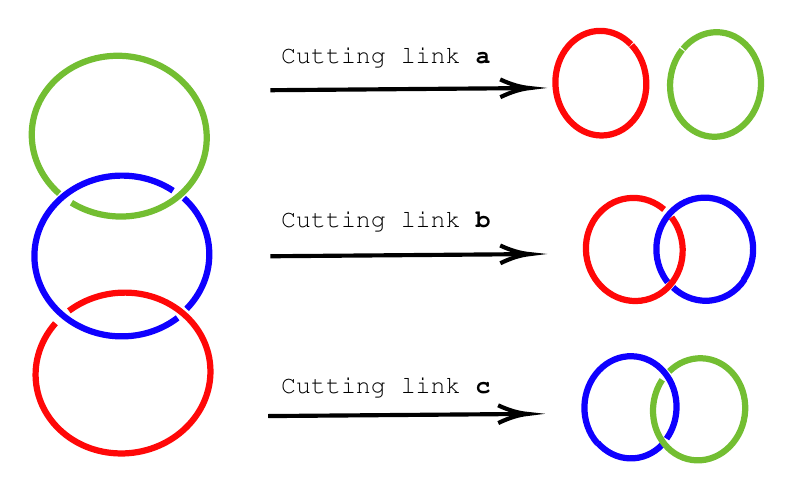
\begin{tikzpicture}[x=0.75pt,y=0.75pt,yscale=-1,xscale=1]
%uncomment if require: \path (0,300); %set diagram left start at 0, and has height of 300

%Shape: Arc [id:dp07834231427117577] 
\draw  [draw opacity=0][line width=2.25]  (167.34,164.68) .. controls (160.27,170.07) and (151.23,173.39) .. (141.34,173.59) .. controls (118.07,174.05) and (98.82,157.09) .. (98.35,135.71) .. controls (97.88,114.33) and (116.36,96.62) .. (139.63,96.15) .. controls (149.14,95.96) and (157.98,98.68) .. (165.14,103.43) -- (140.48,134.87) -- cycle ; \draw  [color={rgb, 255:red, 15; green, 0; blue, 255 }  ,draw opacity=1 ][line width=2.25]  (167.34,164.68) .. controls (160.27,170.07) and (151.23,173.39) .. (141.34,173.59) .. controls (118.07,174.05) and (98.82,157.09) .. (98.35,135.71) .. controls (97.88,114.33) and (116.36,96.62) .. (139.63,96.15) .. controls (149.14,95.96) and (157.98,98.68) .. (165.14,103.43) ;  
%Shape: Arc [id:dp07802046067718771] 
\draw  [draw opacity=0][line width=2.25]  (170.34,106.99) .. controls (177.73,113.67) and (182.37,122.93) .. (182.6,133.3) .. controls (182.83,143.62) and (178.65,153.15) .. (171.65,160.36) -- (140.48,134.87) -- cycle ; \draw  [color={rgb, 255:red, 15; green, 0; blue, 255 }  ,draw opacity=1 ][line width=2.25]  (170.34,106.99) .. controls (177.73,113.67) and (182.37,122.93) .. (182.6,133.3) .. controls (182.83,143.62) and (178.65,153.15) .. (171.65,160.36) ;  
%Shape: Arc [id:dp1431518413580678] 
\draw  [draw opacity=0][line width=2.25]  (114.96,161.32) .. controls (121.92,156.14) and (130.65,152.9) .. (140.19,152.55) .. controls (163.45,151.68) and (182.68,168.32) .. (183.15,189.7) .. controls (183.62,211.08) and (165.15,229.12) .. (141.89,229.98) .. controls (118.63,230.85) and (99.39,214.22) .. (98.92,192.83) .. controls (98.71,183.22) and (102.33,174.28) .. (108.49,167.28) -- (141.04,191.27) -- cycle ; \draw  [color={rgb, 255:red, 255; green, 8; blue, 8 }  ,draw opacity=1 ][line width=2.25]  (114.96,161.32) .. controls (121.92,156.14) and (130.65,152.9) .. (140.19,152.55) .. controls (163.45,151.68) and (182.68,168.32) .. (183.15,189.7) .. controls (183.62,211.08) and (165.15,229.12) .. (141.89,229.98) .. controls (118.63,230.85) and (99.39,214.22) .. (98.92,192.83) .. controls (98.71,183.22) and (102.33,174.28) .. (108.49,167.28) ;  
%Shape: Arc [id:dp1312110151162147] 
\draw  [draw opacity=0][line width=2.25]  (116.19,109.2) .. controls (123.04,113.42) and (131.27,115.88) .. (140.07,115.86) .. controls (163.35,115.81) and (181.84,98.42) .. (181.37,77.03) .. controls (180.89,55.64) and (161.64,38.35) .. (138.36,38.4) .. controls (115.09,38.45) and (96.6,55.83) .. (97.07,77.22) .. controls (97.31,88.03) and (102.34,97.8) .. (110.26,104.81) -- (139.22,77.13) -- cycle ; \draw  [color={rgb, 255:red, 115; green, 190; blue, 50 }  ,draw opacity=1 ][line width=2.25]  (116.19,109.2) .. controls (123.04,113.42) and (131.27,115.88) .. (140.07,115.86) .. controls (163.35,115.81) and (181.84,98.42) .. (181.37,77.03) .. controls (180.89,55.64) and (161.64,38.35) .. (138.36,38.4) .. controls (115.09,38.45) and (96.6,55.83) .. (97.07,77.22) .. controls (97.31,88.03) and (102.34,97.8) .. (110.26,104.81) ;  
%Straight Lines [id:da9656223218785889] 
\draw [line width=1.5]    (212,55) -- (255.98,54.64) -- (334,53.99) ;
\draw [shift={(337,53.97)}, rotate = 179.53] [color={rgb, 255:red, 0; green, 0; blue, 0 }  ][line width=1.5]    (14.21,-4.28) .. controls (9.04,-1.82) and (4.3,-0.39) .. (0,0) .. controls (4.3,0.39) and (9.04,1.82) .. (14.21,4.28)   ;
%Straight Lines [id:da08259161958889605] 
\draw [line width=1.5]    (212,135) -- (255.98,134.64) -- (334,133.99) ;
\draw [shift={(337,133.97)}, rotate = 179.53] [color={rgb, 255:red, 0; green, 0; blue, 0 }  ][line width=1.5]    (14.21,-4.28) .. controls (9.04,-1.82) and (4.3,-0.39) .. (0,0) .. controls (4.3,0.39) and (9.04,1.82) .. (14.21,4.28)   ;
%Straight Lines [id:da9863080107956984] 
\draw [line width=1.5]    (211,212) -- (254.98,211.64) -- (333,210.99) ;
\draw [shift={(336,210.97)}, rotate = 179.53] [color={rgb, 255:red, 0; green, 0; blue, 0 }  ][line width=1.5]    (14.21,-4.28) .. controls (9.04,-1.82) and (4.3,-0.39) .. (0,0) .. controls (4.3,0.39) and (9.04,1.82) .. (14.21,4.28)   ;
%Shape: Arc [id:dp9948335434775479] 
\draw  [draw opacity=0][line width=2.25]  (386.07,33.3) .. controls (390.37,37.91) and (393.09,44.45) .. (393.17,51.69) .. controls (393.31,65.61) and (383.63,76.86) .. (371.53,76.82) .. controls (359.43,76.77) and (349.5,65.46) .. (349.36,51.54) .. controls (349.21,37.62) and (358.9,26.37) .. (371,26.41) .. controls (376.66,26.43) and (381.84,28.91) .. (385.77,32.98) -- (371.26,51.61) -- cycle ; \draw  [color={rgb, 255:red, 255; green, 8; blue, 8 }  ,draw opacity=1 ][line width=2.25]  (386.07,33.3) .. controls (390.37,37.91) and (393.09,44.45) .. (393.17,51.69) .. controls (393.31,65.61) and (383.63,76.86) .. (371.53,76.82) .. controls (359.43,76.77) and (349.5,65.46) .. (349.36,51.54) .. controls (349.21,37.62) and (358.9,26.37) .. (371,26.41) .. controls (376.66,26.43) and (381.84,28.91) .. (385.77,32.98) ;  
%Shape: Arc [id:dp07032538499930807] 
\draw  [draw opacity=0][line width=2.25]  (410.44,35.54) .. controls (406.94,39.96) and (404.75,45.78) .. (404.6,52.16) .. controls (404.29,66.08) and (413.85,77.4) .. (425.95,77.44) .. controls (438.05,77.48) and (448.12,66.23) .. (448.43,52.32) .. controls (448.74,38.4) and (439.19,27.08) .. (427.08,27.04) .. controls (420.75,27.02) and (414.97,30.09) .. (410.86,35.02) -- (426.52,52.24) -- cycle ; \draw  [color={rgb, 255:red, 115; green, 190; blue, 50 }  ,draw opacity=1 ][line width=2.25]  (410.44,35.54) .. controls (406.94,39.96) and (404.75,45.78) .. (404.6,52.16) .. controls (404.29,66.08) and (413.85,77.4) .. (425.95,77.44) .. controls (438.05,77.48) and (448.12,66.23) .. (448.43,52.32) .. controls (448.74,38.4) and (439.19,27.08) .. (427.08,27.04) .. controls (420.75,27.02) and (414.97,30.09) .. (410.86,35.02) ;  
%Shape: Arc [id:dp8695510187382657] 
\draw  [draw opacity=0][line width=2.25]  (403.44,147.53) .. controls (400.13,143.31) and (398.1,137.89) .. (398.01,131.97) .. controls (397.79,118.24) and (408.06,106.96) .. (420.93,106.76) .. controls (433.8,106.56) and (444.41,117.53) .. (444.62,131.25) .. controls (444.71,136.95) and (442.99,142.22) .. (440.03,146.46) -- (421.31,131.61) -- cycle ; \draw  [color={rgb, 255:red, 15; green, 0; blue, 255 }  ,draw opacity=1 ][line width=2.25]  (403.44,147.53) .. controls (400.13,143.31) and (398.1,137.89) .. (398.01,131.97) .. controls (397.79,118.24) and (408.06,106.96) .. (420.93,106.76) .. controls (433.8,106.56) and (444.41,117.53) .. (444.62,131.25) .. controls (444.71,136.95) and (442.99,142.22) .. (440.03,146.46) ;  
%Shape: Arc [id:dp30093039172219116] 
\draw  [draw opacity=0][line width=2.25]  (440.52,146.13) .. controls (436.48,152.28) and (429.81,156.33) .. (422.14,156.45) .. controls (416.02,156.54) and (410.36,154.11) .. (406.07,150.06) -- (421.31,131.61) -- cycle ; \draw  [color={rgb, 255:red, 15; green, 0; blue, 255 }  ,draw opacity=1 ][line width=2.25]  (440.52,146.13) .. controls (436.48,152.28) and (429.81,156.33) .. (422.14,156.45) .. controls (416.02,156.54) and (410.36,154.11) .. (406.07,150.06) ;  
%Shape: Arc [id:dp8029802001836879] 
\draw  [draw opacity=0][line width=2.25]  (405.32,116.27) .. controls (408.5,120.42) and (410.48,125.66) .. (410.67,131.37) .. controls (411.13,145.09) and (401.07,156.37) .. (388.2,156.57) .. controls (375.33,156.77) and (364.53,145.8) .. (364.07,132.09) .. controls (363.61,118.37) and (373.67,107.08) .. (386.54,106.89) .. controls (392.24,106.8) and (397.54,108.9) .. (401.71,112.46) -- (387.37,131.73) -- cycle ; \draw  [color={rgb, 255:red, 255; green, 8; blue, 8 }  ,draw opacity=1 ][line width=2.25]  (405.32,116.27) .. controls (408.5,120.42) and (410.48,125.66) .. (410.67,131.37) .. controls (411.13,145.09) and (401.07,156.37) .. (388.2,156.57) .. controls (375.33,156.77) and (364.53,145.8) .. (364.07,132.09) .. controls (363.61,118.37) and (373.67,107.08) .. (386.54,106.89) .. controls (392.24,106.8) and (397.54,108.9) .. (401.71,112.46) ;  
%Shape: Arc [id:dp03635674066481054] 
\draw  [draw opacity=0][line width=2.25]  (369.75,225.23) .. controls (365.6,220.62) and (363.12,214.17) .. (363.35,207.11) .. controls (363.79,193.52) and (374.08,182.8) .. (386.33,183.16) .. controls (398.58,183.52) and (408.15,194.83) .. (407.71,208.42) .. controls (407.53,213.89) and (405.76,218.89) .. (402.9,222.9) -- (385.53,207.76) -- cycle ; \draw  [color={rgb, 255:red, 15; green, 0; blue, 255 }  ,draw opacity=1 ][line width=2.25]  (369.75,225.23) .. controls (365.6,220.62) and (363.12,214.17) .. (363.35,207.11) .. controls (363.79,193.52) and (374.08,182.8) .. (386.33,183.16) .. controls (398.58,183.52) and (408.15,194.83) .. (407.71,208.42) .. controls (407.53,213.89) and (405.76,218.89) .. (402.9,222.9) ;  
%Shape: Arc [id:dp5441819996566084] 
\draw  [draw opacity=0][line width=2.25]  (400.74,225.85) .. controls (396.67,230.05) and (391.17,232.56) .. (385.15,232.38) .. controls (379.17,232.2) and (373.78,229.41) .. (369.85,225.01) -- (385.53,207.76) -- cycle ; \draw  [color={rgb, 255:red, 15; green, 0; blue, 255 }  ,draw opacity=1 ][line width=2.25]  (400.74,225.85) .. controls (396.67,230.05) and (391.17,232.56) .. (385.15,232.38) .. controls (379.17,232.2) and (373.78,229.41) .. (369.85,225.01) ;  
%Shape: Arc [id:dp8213345284708432] 
\draw  [draw opacity=0][line width=2.25]  (400.83,194.53) .. controls (398.27,198.37) and (396.67,203.03) .. (396.42,208.08) .. controls (395.74,221.66) and (405.13,232.97) .. (417.38,233.33) .. controls (429.63,233.69) and (440.11,222.97) .. (440.78,209.39) .. controls (441.45,195.81) and (432.07,184.51) .. (419.82,184.15) .. controls (413.89,183.97) and (408.38,186.39) .. (404.2,190.47) -- (418.6,208.74) -- cycle ; \draw  [color={rgb, 255:red, 115; green, 190; blue, 50 }  ,draw opacity=1 ][line width=2.25]  (400.83,194.53) .. controls (398.27,198.37) and (396.67,203.03) .. (396.42,208.08) .. controls (395.74,221.66) and (405.13,232.97) .. (417.38,233.33) .. controls (429.63,233.69) and (440.11,222.97) .. (440.78,209.39) .. controls (441.45,195.81) and (432.07,184.51) .. (419.82,184.15) .. controls (413.89,183.97) and (408.38,186.39) .. (404.2,190.47) ;  

% Text Node
\draw (216,33) node [anchor=north west][inner sep=0.75pt]  [font=\small] [align=left] {{\fontfamily{pcr}\selectfont Cutting link \textbf{a}}};
% Text Node
\draw (216,112) node [anchor=north west][inner sep=0.75pt]  [font=\small] [align=left] {{\fontfamily{pcr}\selectfont Cutting link \textbf{b}}};
% Text Node
\draw (216,192) node [anchor=north west][inner sep=0.75pt]  [font=\small] [align=left] {{\fontfamily{pcr}\selectfont Cutting link \textbf{c}}};


\end{tikzpicture}
}
                \caption{Possible link cuts for the $3^3$ link class. One cut lead to complete separability while two of the cuts lead to entangled configurations.}
            \end{figure}
            \noindent   
\textbf{\large \texttt{3\textsuperscript{4}} Link Class} \\[0.3cm]
Let us now analyse the class $P_4(a,b,c) = ab+ac+bc$. The link diagram is given by:
\begin{figure}[H]
    \centering
  

\tikzset{every picture/.style={line width=0.75pt}} %set default line width to 0.75pt        

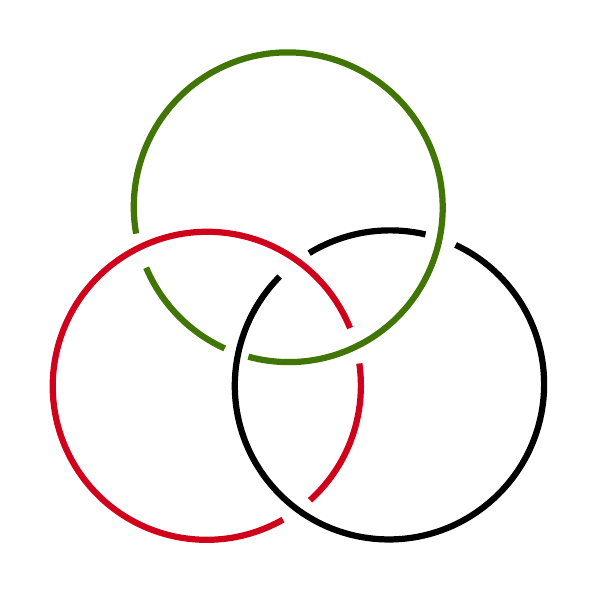
\begin{tikzpicture}[x=0.75pt,y=0.75pt,yscale=-1,xscale=1]
%uncomment if require: \path (0,300); %set diagram left start at 0, and has height of 300

%Shape: Arc [id:dp5841759180684423] 
\draw  [draw opacity=0][line width=2.25]  (290.27,165.55) .. controls (273.28,157.84) and (259.7,143.9) .. (252.41,126.63) -- (320.87,97.51) -- cycle ; \draw  [color={rgb, 255:red, 65; green, 117; blue, 5 }  ,draw opacity=1 ][line width=2.25]  (290.27,165.55) .. controls (273.28,157.84) and (259.7,143.9) .. (252.41,126.63) ;  
%Shape: Arc [id:dp7577998399786959] 
\draw  [draw opacity=0][line width=2.25]  (401.49,115.68) .. controls (411.67,120.44) and (420.91,127.58) .. (428.32,137) .. controls (453.68,169.27) and (447.97,216.08) .. (415.56,241.55) .. controls (383.16,267.03) and (336.33,261.52) .. (310.96,229.25) .. controls (287.54,199.45) and (290.62,157.26) .. (316.74,130.91) -- (369.64,183.13) -- cycle ; \draw  [color={rgb, 255:red, 0; green, 0; blue, 0 }  ,draw opacity=1 ][line width=2.25]  (401.49,115.68) .. controls (411.67,120.44) and (420.91,127.58) .. (428.32,137) .. controls (453.68,169.27) and (447.97,216.08) .. (415.56,241.55) .. controls (383.16,267.03) and (336.33,261.52) .. (310.96,229.25) .. controls (287.54,199.45) and (290.62,157.26) .. (316.74,130.91) ;  
%Shape: Arc [id:dp896095108426711] 
\draw  [draw opacity=0][line width=2.25]  (247.58,110.23) .. controls (241.88,77.87) and (258.12,44.5) .. (289.17,29.93) .. controls (326.35,12.5) and (370.67,28.62) .. (388.18,65.94) .. controls (405.69,103.27) and (389.75,147.66) .. (352.57,165.1) .. controls (336.02,172.86) and (318.05,173.97) .. (301.66,169.52) -- (320.87,97.51) -- cycle ; \draw  [color={rgb, 255:red, 65; green, 117; blue, 5 }  ,draw opacity=1 ][line width=2.25]  (247.58,110.23) .. controls (241.88,77.87) and (258.12,44.5) .. (289.17,29.93) .. controls (326.35,12.5) and (370.67,28.62) .. (388.18,65.94) .. controls (405.69,103.27) and (389.75,147.66) .. (352.57,165.1) .. controls (336.02,172.86) and (318.05,173.97) .. (301.66,169.52) ;  
%Shape: Arc [id:dp5765147440419169] 
\draw  [draw opacity=0][line width=2.25]  (318.33,248.02) .. controls (282.68,268.27) and (237.38,255.9) .. (217.12,220.36) .. controls (196.83,184.78) and (209.3,139.45) .. (244.97,119.12) .. controls (280.64,98.78) and (326,111.14) .. (346.28,146.72) .. controls (347.96,149.66) and (349.41,152.67) .. (350.65,155.72) -- (281.7,183.54) -- cycle ; \draw  [color={rgb, 255:red, 208; green, 2; blue, 27 }  ,draw opacity=1 ][line width=2.25]  (318.33,248.02) .. controls (282.68,268.27) and (237.38,255.9) .. (217.12,220.36) .. controls (196.83,184.78) and (209.3,139.45) .. (244.97,119.12) .. controls (280.64,98.78) and (326,111.14) .. (346.28,146.72) .. controls (347.96,149.66) and (349.41,152.67) .. (350.65,155.72) ;  
%Shape: Arc [id:dp9828413593386676] 
\draw  [draw opacity=0][line width=2.25]  (330.95,119.62) .. controls (347.94,109.22) and (368.18,106.21) .. (387.01,110.62) -- (369.64,183.13) -- cycle ; \draw  [color={rgb, 255:red, 0; green, 0; blue, 0 }  ,draw opacity=1 ][line width=2.25]  (330.95,119.62) .. controls (347.94,109.22) and (368.18,106.21) .. (387.01,110.62) ;  
%Shape: Arc [id:dp23316225635631627] 
\draw  [draw opacity=0][line width=2.25]  (355.12,172.79) .. controls (356.17,180.07) and (356.16,187.63) .. (354.93,195.28) .. controls (352.14,212.7) and (343.51,227.73) .. (331.38,238.69) -- (281.7,183.54) -- cycle ; \draw  [color={rgb, 255:red, 208; green, 2; blue, 27 }  ,draw opacity=1 ][line width=2.25]  (355.12,172.79) .. controls (356.17,180.07) and (356.16,187.63) .. (354.93,195.28) .. controls (352.14,212.7) and (343.51,227.73) .. (331.38,238.69) ;  




\end{tikzpicture}
  
  \caption{The knot diagram, characterising the $3^4$ link class.}
\end{figure}
\noindent
This link demostrates a behaviour opposite to that of the Borromean ring, that is, setting any one variable to zero with not result in complete separability. The other two links remain entangled. The pure state having the characteristic of the link is the \textbf{W state} which has been documented in previous works:
$$\ket{3^4} = \frac{1}{\sqrt{3}}\brac{\ket{001}_{abc}+\ket{010}_{abc}+\ket{100}_{abc}}$$ 
Let us check whether this state satisfies the link property. The density matrix is given by:
\begin{equation*}
    \rho{abc}=
    \left[
    \begin{array}{cccccccc}
    0.0 & 0.0 & 0.0 & 0.0 & 0.0 & 0.0 & 0.0 & 0.0 \\
    0.0 & 0.333 & 0.333 & 0.0 & 0.333 & 0.0 & 0.0 & 0.0 \\
    0.0 & 0.333 & 0.333 & 0.0 & 0.333 & 0.0 & 0.0 & 0.0 \\
    0.0 & 0.0 & 0.0 & 0.0 & 0.0 & 0.0 & 0.0 & 0.0 \\
    0.0 & 0.333 & 0.333 & 0.0 & 0.333 & 0.0 & 0.0 & 0.0 \\
    0.0 & 0.0 & 0.0 & 0.0 & 0.0 & 0.0 & 0.0 & 0.0 \\
    0.0 & 0.0 & 0.0 & 0.0 & 0.0 & 0.0 & 0.0 & 0.0 \\
    0.0 & 0.0 & 0.0 & 0.0 & 0.0 & 0.0 & 0.0 & 0.0 \\
    \end{array}
    \right]
    \end{equation*}
    The corresponding partial transpose with respect to the three variables are given by:
    \begin{equation*}
        \rho^{T_a}_{abc} =
        \left[
        \begin{array}{cccccccc}
        0.0 & 0.0 & 0.0 & 0.0 & 0.0 & 0.333 & 0.333 & 0.0 \\
        0.0 & 0.333 & 0.333 & 0.0 & 0.0 & 0.0 & 0.0 & 0.0 \\
        0.0 & 0.333 & 0.333 & 0.0 & 0.0 & 0.0 & 0.0 & 0.0 \\
        0.0 & 0.0 & 0.0 & 0.0 & 0.0 & 0.0 & 0.0 & 0.0 \\
        0.0 & 0.0 & 0.0 & 0.0 & 0.333 & 0.0 & 0.0 & 0.0 \\
        0.333 & 0.0 & 0.0 & 0.0 & 0.0 & 0.0 & 0.0 & 0.0 \\
        0.333 & 0.0 & 0.0 & 0.0 & 0.0 & 0.0 & 0.0 & 0.0 \\
        0.0 & 0.0 & 0.0 & 0.0 & 0.0 & 0.0 & 0.0 & 0.0 \\
        \end{array}
        \right]
        \end{equation*}
        \begin{equation*}
            \rho^{T_b}_{abc}=
            \left[
            \begin{array}{cccccccc}
            0.0 & 0.0 & 0.0 & 0.333 & 0.0 & 0.0 & 0.333 & 0.0 \\
            0.0 & 0.333 & 0.0 & 0.0 & 0.333 & 0.0 & 0.0 & 0.0 \\
            0.0 & 0.0 & 0.333 & 0.0 & 0.0 & 0.0 & 0.0 & 0.0 \\
            0.333 & 0.0 & 0.0 & 0.0 & 0.0 & 0.0 & 0.0 & 0.0 \\
            0.0 & 0.333 & 0.0 & 0.0 & 0.333 & 0.0 & 0.0 & 0.0 \\
            0.0 & 0.0 & 0.0 & 0.0 & 0.0 & 0.0 & 0.0 & 0.0 \\
            0.333 & 0.0 & 0.0 & 0.0 & 0.0 & 0.0 & 0.0 & 0.0 \\
            0.0 & 0.0 & 0.0 & 0.0 & 0.0 & 0.0 & 0.0 & 0.0 \\
            \end{array}
            \right]
            \end{equation*}
            \begin{equation*}
                \rho^{T_c}_{abc}=
                \left[
                \begin{array}{cccccccc}
                0.0 & 0.0 & 0.0 & 0.333 & 0.0 & 0.333 & 0.0 & 0.0 \\
                0.0 & 0.333 & 0.0 & 0.0 & 0.0 & 0.0 & 0.0 & 0.0 \\
                0.0 & 0.0 & 0.333 & 0.0 & 0.333 & 0.0 & 0.0 & 0.0 \\
                0.333 & 0.0 & 0.0 & 0.0 & 0.0 & 0.0 & 0.0 & 0.0 \\
                0.0 & 0.0 & 0.333 & 0.0 & 0.333 & 0.0 & 0.0 & 0.0 \\
                0.333 & 0.0 & 0.0 & 0.0 & 0.0 & 0.0 & 0.0 & 0.0 \\
                0.0 & 0.0 & 0.0 & 0.0 & 0.0 & 0.0 & 0.0 & 0.0 \\
                0.0 & 0.0 & 0.0 & 0.0 & 0.0 & 0.0 & 0.0 & 0.0 \\
                \end{array}
                \right]
                \end{equation*}
               All the three matrices have the same set of eigenvalues $\mathbf{\mathcolor{red}{-0.471}}, 0.0, 0.333, 0.471, 0.666$, one of which is negative, thus denoting the presence of entanglement. The reduced density matrix in each case is the same and is given by:
               \begin{equation*}
                \rho_{reduced} =
                \left[
                \begin{array}{cccc}
                0.333 & 0.0 & 0.0 & 0.333 \\
                0.0 & 0.333 & 0.0 & 0.0 \\
                0.0 & 0.0 & 0.333 & 0.0 \\
                0.333 & 0.0 & 0.0 & 0.0 \\
                \end{array}
                \right]
                \end{equation*}
                The partial transpose of this is the same as that of the matrix. The eigenvalues of the PPT matrix are $-0.206, 0.333, 0.333, 0.539$, one of which is negative, thus denoting the present of entanglement. This verifies the behaviour of the link $ab+ac+bc$. \\[0.3cm]
From the algorithm, the mixed state can be obtained using the state:
$$\ket{\psi_4} = \ket{2^1}_{ab}\ket{0}_c\ket{0}_d+\ket{2^1}_{ac}\ket{1}_b\ket{1}_d+\ket{2^1}_{bc}\ket{0}_a\ket{2}_d$$
Using the above state after tracing out subsystem $d$, we obtained the density matrix as:
\begin{equation*}
    \rho_{abc}=
    \left[
    \begin{array}{cccccccc}
    0.25 & 0.0 & 0.0 & 0.125 & 0.0 & 0.0 & 0.125 & 0.0 \\
    0.0 & 0.0 & 0.0 & 0.0 & 0.0 & 0.0 & 0.0 & 0.0 \\
    0.0 & 0.0 & 0.25 & 0.0 & 0.0 & 0.0 & 0.0 & 0.25 \\
    0.125 & 0.0 & 0.0 & 0.125 & 0.0 & 0.0 & 0.0 & 0.0 \\
    0.0 & 0.0 & 0.0 & 0.0 & 0.0 & 0.0 & 0.0 & 0.0 \\
    0.0 & 0.0 & 0.0 & 0.0 & 0.0 & 0.0 & 0.0 & 0.0 \\
    0.125 & 0.0 & 0.0 & 0.0 & 0.0 & 0.0 & 0.125 & 0.0 \\
    0.0 & 0.0 & 0.25 & 0.0 & 0.0 & 0.0 & 0.0 & 0.25 \\
    \end{array}
    \right]
    \end{equation*}
    Let us now check the partial transpose for the entire system. The PPT matrices are found to be:\\
    \begin{align*}
        \rho^{T_a}_{abc} &=
        \left[
        \begin{array}{cccccccc}
        0.25 & 0.0 & 0.0 & 0.125 & 0.0 & 0.0 & 0.0 & 0.0 \\
        0.0 & 0.0 & 0.0 & 0.0 & 0.0 & 0.0 & 0.0 & 0.0 \\
        0.0 & 0.0 & 0.25 & 0.0 & 0.125 & 0.0 & 0.0 & 0.0 \\
        0.125 & 0.0 & 0.0 & 0.125 & 0.0 & 0.0 & 0.25 & 0.0 \\
        0.0 & 0.0 & 0.125 & 0.0 & 0.0 & 0.0 & 0.0 & 0.0 \\
        0.0 & 0.0 & 0.0 & 0.0 & 0.0 & 0.0 & 0.0 & 0.0 \\
        0.0 & 0.0 & 0.0 & 0.25 & 0.0 & 0.0 & 0.125 & 0.0 \\
        0.0 & 0.0 & 0.0 & 0.0 & 0.0 & 0.0 & 0.0 & 0.25 \\
        \end{array}
        \right]   \\
        \rho^{T_b}_{abc} &=
        \left[
        \begin{array}{cccccccc}
        0.25 & 0.0 & 0.0 & 0.0 & 0.0 & 0.0 & 0.0 & 0.0 \\
        0.0 & 0.0 & 0.125 & 0.0 & 0.0 & 0.0 & 0.0 & 0.0 \\
        0.0 & 0.125 & 0.25 & 0.0 & 0.125 & 0.0 & 0.0 & 0.25 \\
        0.0 & 0.0 & 0.0 & 0.125 & 0.0 & 0.0 & 0.0 & 0.0 \\
        0.0 & 0.0 & 0.125 & 0.0 & 0.0 & 0.0 & 0.0 & 0.0 \\
        0.0 & 0.0 & 0.0 & 0.0 & 0.0 & 0.0 & 0.0 & 0.0 \\
        0.0 & 0.0 & 0.0 & 0.0 & 0.0 & 0.0 & 0.125 & 0.0 \\
        0.0 & 0.0 & 0.25 & 0.0 & 0.0 & 0.0 & 0.0 & 0.25 \\
        \end{array}
        \right]\\
        \rho^{T_c}_{abc} &=
        \left[
        \begin{array}{cccccccc}
        0.25 & 0.0 & 0.0 & 0.0 & 0.0 & 0.0 & 0.125 & 0.0 \\
        0.0 & 0.0 & 0.125 & 0.0 & 0.0 & 0.0 & 0.0 & 0.0 \\
        0.0 & 0.125 & 0.25 & 0.0 & 0.0 & 0.0 & 0.0 & 0.0 \\
        0.0 & 0.0 & 0.0 & 0.125 & 0.0 & 0.0 & 0.25 & 0.0 \\
        0.0 & 0.0 & 0.0 & 0.0 & 0.0 & 0.0 & 0.0 & 0.0 \\
        0.0 & 0.0 & 0.0 & 0.0 & 0.0 & 0.0 & 0.0 & 0.0 \\
        0.125 & 0.0 & 0.0 & 0.25 & 0.0 & 0.0 & 0.125 & 0.0 \\
        0.0 & 0.0 & 0.0 & 0.0 & 0.0 & 0.0 & 0.0 & 0.25 \\
        \end{array}
        \right]
        \end{align*}
        The set of eigenvalues of $\rho^{T_a}_{abc}$ and $\rho^{T_c}_{abc}$ are the same, namely $\mathcolor{red}{\mathbf{-0.146}}, \mathcolor{red}{\mathbf{-0.052}}, 0.0, 0.0, 0.222, 0.25, 0.302,\\ 0.424$ while the eigenvalues of $\rho^{T_b}_{abc}$ are $\mathcolor{red}{\mathbf{-0.138}}, 0.0, 0.0, 0.107, 0.125, 0.125, 0.25, 0.531$. We see that there exists atleast one negative eigenvalue in all the three matrices, thus denoting the presence of tripartite entanglement. Let us now check the reduced density matrices. 

        \begin{align*}
            \rho_{bc} &=
            \left[
            \begin{array}{cccc}
            0.25 & 0.0 & 0.0 & 0.125 \\
            0.0 & 0.0 & 0.0 & 0.0 \\
            0.0 & 0.0 & 0.375 & 0.0 \\
            0.125 & 0.0 & 0.0 & 0.375 \\
            \end{array}
            \right]\quad \rho_{bc}^{T_b} = 
            \left[
                \begin{array}{cccc}
                0.25 & 0.0 & 0.0 & 0.0 \\
                0.0 & 0.0 & 0.125 & 0.0 \\
                0.0 & 0.125 & 0.375 & 0.0 \\
                0.0 & 0.0 & 0.0 & 0.375 \\
                \end{array}
                \right]
                \\
            \rho_{ac} &=
            \left[
            \begin{array}{cccc}
            0.5 & 0.0 & 0.0 & 0.25 \\
            0.0 & 0.125 & 0.0 & 0.0 \\
            0.0 & 0.0 & 0.125 & 0.0 \\
            0.25 & 0.0 & 0.0 & 0.25 \\
            \end{array}
            \right]\quad \rho_{ac}^{Ta}= \left[
                \begin{array}{cccc}
                0.5 & 0.0 & 0.0 & 0.0 \\
                0.0 & 0.125 & 0.25 & 0.0 \\
                0.0 & 0.25 & 0.125 & 0.0 \\
                0.0 & 0.0 & 0.0 & 0.25 \\
                \end{array}
                \right]\\
            \rho_{ab} &=
            \left[
            \begin{array}{cccc}
            0.25 & 0.0 & 0.0 & 0.125 \\
            0.0 & 0.375 & 0.0 & 0.0 \\
            0.0 & 0.0 & 0.0 & 0.0 \\
            0.125 & 0.0 & 0.0 & 0.375 \\
            \end{array}
            \right]\quad \rho_{ab}^{T_a} = \left[
                \begin{array}{cccc}
                0.25 & 0.0 & 0.0 & 0.0 \\
                0.0 & 0.375 & 0.125 & 0.0 \\
                0.0 & 0.125 & 0.0 & 0.0 \\
                0.0 & 0.0 & 0.0 & 0.375 \\
                \end{array}
                \right]
            \end{align*}
           The set of eigenvalues of PPT matrices of $\rho_{bc}$ and $\rho_{ab}$ are the same given by $\mathcolor{red}{\mathbf{-0.038}}, 0.25, 0.375, 0.413$ while the eigenvalues of PPT matrix of $\rho_{ac}$ are $\mathcolor{red}{\mathbf{-0.125}}, 0.25, 0.375, 0.5$. Since in each set, a negative eigenvalue exists, we can conclude that the system exhibits entanglement, thus verifying the behaviour of the link $ab+ac+bc$, that is, even after cutting one variable, the other two remain entangled.
            

           \begin{figure}[H]
            \centering
            \scalebox{0.8}{ 

\tikzset{every picture/.style={line width=0.75pt}} %set default line width to 0.75pt        

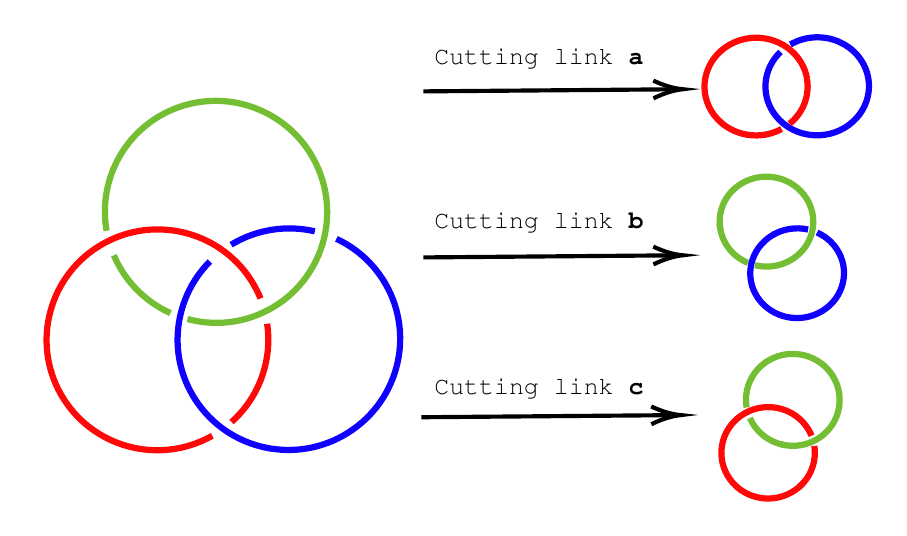
\begin{tikzpicture}[x=0.75pt,y=0.75pt,yscale=-1,xscale=1]
%uncomment if require: \path (0,300); %set diagram left start at 0, and has height of 300

%Shape: Arc [id:dp4773851197196687] 
\draw  [draw opacity=0][line width=2.25]  (121.14,167.84) .. controls (108.91,162.33) and (99.12,152.35) .. (93.85,139.98) -- (143.09,119.04) -- cycle ; \draw  [color={rgb, 255:red, 115; green, 190; blue, 50 }  ,draw opacity=1 ][line width=2.25]  (121.14,167.84) .. controls (108.91,162.33) and (99.12,152.35) .. (93.85,139.98) ;  
%Shape: Arc [id:dp7253265627788676] 
\draw  [draw opacity=0][line width=2.25]  (201.09,132.06) .. controls (208.42,135.46) and (215.07,140.58) .. (220.41,147.35) .. controls (238.66,170.47) and (234.55,204.02) .. (211.23,222.28) .. controls (187.91,240.54) and (154.21,236.6) .. (135.96,213.47) .. controls (119.1,192.11) and (121.32,161.86) .. (140.12,142.97) -- (178.18,180.41) -- cycle ; \draw  [color={rgb, 255:red, 15; green, 0; blue, 255 }  ,draw opacity=1 ][line width=2.25]  (201.09,132.06) .. controls (208.42,135.46) and (215.07,140.58) .. (220.41,147.35) .. controls (238.66,170.47) and (234.55,204.02) .. (211.23,222.28) .. controls (187.91,240.54) and (154.21,236.6) .. (135.96,213.47) .. controls (119.1,192.11) and (121.32,161.86) .. (140.12,142.97) ;  
%Shape: Arc [id:dp9192874489288929] 
\draw  [draw opacity=0][line width=2.25]  (90.35,128.13) .. controls (86.26,104.94) and (97.95,81.03) .. (120.28,70.59) .. controls (147.03,58.09) and (178.93,69.65) .. (191.53,96.4) .. controls (204.13,123.16) and (192.65,154.99) .. (165.9,167.49) .. controls (154.01,173.05) and (141.1,173.85) .. (129.33,170.68) -- (143.09,119.04) -- cycle ; \draw  [color={rgb, 255:red, 115; green, 190; blue, 50 }  ,draw opacity=1 ][line width=2.25]  (90.35,128.13) .. controls (86.26,104.94) and (97.95,81.03) .. (120.28,70.59) .. controls (147.03,58.09) and (178.93,69.65) .. (191.53,96.4) .. controls (204.13,123.16) and (192.65,154.99) .. (165.9,167.49) .. controls (154.01,173.05) and (141.1,173.85) .. (129.33,170.68) ;  
%Shape: Arc [id:dp042875124104498785] 
\draw  [draw opacity=0][line width=2.25]  (141.27,226.92) .. controls (115.61,241.44) and (83.02,232.58) .. (68.44,207.1) .. controls (53.84,181.59) and (62.8,149.1) .. (88.47,134.52) .. controls (114.13,119.94) and (146.77,128.8) .. (161.37,154.3) .. controls (162.58,156.42) and (163.63,158.58) .. (164.52,160.77) -- (114.9,180.7) -- cycle ; \draw  [color={rgb, 255:red, 255; green, 8; blue, 8 }  ,draw opacity=1 ][line width=2.25]  (141.27,226.92) .. controls (115.61,241.44) and (83.02,232.58) .. (68.44,207.1) .. controls (53.84,181.59) and (62.8,149.1) .. (88.47,134.52) .. controls (114.13,119.94) and (146.77,128.8) .. (161.37,154.3) .. controls (162.58,156.42) and (163.63,158.58) .. (164.52,160.77) ;  
%Shape: Arc [id:dp16987179979790257] 
\draw  [draw opacity=0][line width=2.25]  (150.35,134.89) .. controls (162.57,127.43) and (177.14,125.27) .. (190.69,128.44) -- (178.18,180.41) -- cycle ; \draw  [color={rgb, 255:red, 15; green, 0; blue, 255 }  ,draw opacity=1 ][line width=2.25]  (150.35,134.89) .. controls (162.57,127.43) and (177.14,125.27) .. (190.69,128.44) ;  
%Shape: Arc [id:dp6029343238857104] 
\draw  [draw opacity=0][line width=2.25]  (167.72,172.94) .. controls (168.49,178.17) and (168.48,183.61) .. (167.6,189.11) .. controls (165.58,201.63) and (159.35,212.43) .. (150.57,220.29) -- (114.9,180.7) -- cycle ; \draw  [color={rgb, 255:red, 255; green, 8; blue, 8 }  ,draw opacity=1 ][line width=2.25]  (167.72,172.94) .. controls (168.49,178.17) and (168.48,183.61) .. (167.6,189.11) .. controls (165.58,201.63) and (159.35,212.43) .. (150.57,220.29) ;  
%Straight Lines [id:da7534556779978497] 
\draw [line width=1.5]    (243,61) -- (286.98,60.64) -- (365,59.99) ;
\draw [shift={(368,59.97)}, rotate = 179.53] [color={rgb, 255:red, 0; green, 0; blue, 0 }  ][line width=1.5]    (14.21,-4.28) .. controls (9.04,-1.82) and (4.3,-0.39) .. (0,0) .. controls (4.3,0.39) and (9.04,1.82) .. (14.21,4.28)   ;
%Straight Lines [id:da5964379397474552] 
\draw [line width=1.5]    (243,141) -- (286.98,140.64) -- (365,139.99) ;
\draw [shift={(368,139.97)}, rotate = 179.53] [color={rgb, 255:red, 0; green, 0; blue, 0 }  ][line width=1.5]    (14.21,-4.28) .. controls (9.04,-1.82) and (4.3,-0.39) .. (0,0) .. controls (4.3,0.39) and (9.04,1.82) .. (14.21,4.28)   ;
%Straight Lines [id:da3238547254940084] 
\draw [line width=1.5]    (242,218) -- (285.98,217.64) -- (364,216.99) ;
\draw [shift={(367,216.97)}, rotate = 179.53] [color={rgb, 255:red, 0; green, 0; blue, 0 }  ][line width=1.5]    (14.21,-4.28) .. controls (9.04,-1.82) and (4.3,-0.39) .. (0,0) .. controls (4.3,0.39) and (9.04,1.82) .. (14.21,4.28)   ;
%Shape: Arc [id:dp27861944071878575] 
\draw  [draw opacity=0][line width=2.25]  (443.29,37.13) .. controls (446.74,38.64) and (449.87,40.92) .. (452.38,43.93) .. controls (460.87,54.17) and (458.95,69.01) .. (448.11,77.09) .. controls (437.26,85.17) and (421.59,83.43) .. (413.1,73.19) .. controls (405.25,63.73) and (406.29,50.33) .. (415.06,41.98) -- (432.74,58.56) -- cycle ; \draw  [color={rgb, 255:red, 15; green, 0; blue, 255 }  ,draw opacity=1 ][line width=2.25]  (443.29,37.13) .. controls (446.74,38.64) and (449.87,40.92) .. (452.38,43.93) .. controls (460.87,54.17) and (458.95,69.01) .. (448.11,77.09) .. controls (437.26,85.17) and (421.59,83.43) .. (413.1,73.19) .. controls (405.25,63.73) and (406.29,50.33) .. (415.06,41.98) ;  
%Shape: Arc [id:dp3246032835989415] 
\draw  [draw opacity=0][line width=2.25]  (415.56,79.14) .. controls (403.63,85.57) and (388.47,81.65) .. (381.68,70.37) .. controls (374.89,59.09) and (379.07,44.71) .. (391,38.26) .. controls (402.94,31.81) and (418.13,35.73) .. (424.92,47.02) .. controls (426.46,49.58) and (427.44,52.3) .. (427.88,55.05) -- (403.3,58.69) -- cycle ; \draw  [color={rgb, 255:red, 255; green, 8; blue, 8 }  ,draw opacity=1 ][line width=2.25]  (415.56,79.14) .. controls (403.63,85.57) and (388.47,81.65) .. (381.68,70.37) .. controls (374.89,59.09) and (379.07,44.71) .. (391,38.26) .. controls (402.94,31.81) and (418.13,35.73) .. (424.92,47.02) .. controls (426.46,49.58) and (427.44,52.3) .. (427.88,55.05) ;  
%Shape: Arc [id:dp6977384256640647] 
\draw  [draw opacity=0][line width=2.25]  (419.8,38.42) .. controls (427.01,34.24) and (435.97,33.83) .. (443.49,37.2) -- (432.74,58.56) -- cycle ; \draw  [color={rgb, 255:red, 15; green, 0; blue, 255 }  ,draw opacity=1 ][line width=2.25]  (419.8,38.42) .. controls (427.01,34.24) and (435.97,33.83) .. (443.49,37.2) ;  
%Shape: Arc [id:dp17478235887856808] 
\draw  [draw opacity=0][line width=2.25]  (427.82,54.94) .. controls (428.23,57.35) and (428.24,59.87) .. (427.81,62.42) .. controls (426.84,68.15) and (423.77,73.07) .. (419.46,76.58) -- (403.3,58.69) -- cycle ; \draw  [color={rgb, 255:red, 255; green, 8; blue, 8 }  ,draw opacity=1 ][line width=2.25]  (427.82,54.94) .. controls (428.23,57.35) and (428.24,59.87) .. (427.81,62.42) .. controls (426.84,68.15) and (423.77,73.07) .. (419.46,76.58) ;  
%Shape: Arc [id:dp8901695254096645] 
\draw  [draw opacity=0][line width=2.25]  (399.34,143.64) .. controls (391.55,140.4) and (386.04,133.05) .. (385.76,124.44) -- (408.28,123.75) -- cycle ; \draw  [color={rgb, 255:red, 115; green, 190; blue, 50 }  ,draw opacity=1 ][line width=2.25]  (399.34,143.64) .. controls (391.55,140.4) and (386.04,133.05) .. (385.76,124.44) ;  
%Shape: Arc [id:dp03862703000234913] 
\draw  [draw opacity=0][line width=2.25]  (432.64,128.99) .. controls (435.76,130.37) and (438.59,132.45) .. (440.85,135.21) .. controls (448.54,144.58) and (446.81,158.17) .. (436.99,165.57) .. controls (427.17,172.96) and (412.97,171.37) .. (405.28,162) .. controls (397.59,152.63) and (399.32,139.04) .. (409.15,131.65) .. controls (410.15,130.89) and (411.2,130.23) .. (412.28,129.66) -- (423.07,148.61) -- cycle ; \draw  [color={rgb, 255:red, 15; green, 0; blue, 255 }  ,draw opacity=1 ][line width=2.25]  (432.64,128.99) .. controls (435.76,130.37) and (438.59,132.45) .. (440.85,135.21) .. controls (448.54,144.58) and (446.81,158.17) .. (436.99,165.57) .. controls (427.17,172.96) and (412.97,171.37) .. (405.28,162) .. controls (397.59,152.63) and (399.32,139.04) .. (409.15,131.65) .. controls (410.15,130.89) and (411.2,130.23) .. (412.28,129.66) ;  
%Shape: Arc [id:dp037718546478421766] 
\draw  [draw opacity=0][line width=2.25]  (386.04,127.29) .. controls (384.39,117.94) and (389.31,108.33) .. (398.68,104.13) .. controls (409.94,99.06) and (423.38,103.74) .. (428.69,114.58) .. controls (434,125.42) and (429.16,138.31) .. (417.89,143.37) .. controls (412.98,145.58) and (407.65,145.94) .. (402.76,144.74) -- (408.28,123.75) -- cycle ; \draw  [color={rgb, 255:red, 115; green, 190; blue, 50 }  ,draw opacity=1 ][line width=2.25]  (386.04,127.29) .. controls (384.39,117.94) and (389.31,108.33) .. (398.68,104.13) .. controls (409.94,99.06) and (423.38,103.74) .. (428.69,114.58) .. controls (434,125.42) and (429.16,138.31) .. (417.89,143.37) .. controls (412.98,145.58) and (407.65,145.94) .. (402.76,144.74) ;  
%Shape: Arc [id:dp8813673871140711] 
\draw  [draw opacity=0][line width=2.25]  (411.35,130.17) .. controls (416.5,127.15) and (422.64,126.27) .. (428.35,127.56) -- (423.07,148.61) -- cycle ; \draw  [color={rgb, 255:red, 15; green, 0; blue, 255 }  ,draw opacity=1 ][line width=2.25]  (411.35,130.17) .. controls (416.5,127.15) and (422.64,126.27) .. (428.35,127.56) ;  
%Shape: Arc [id:dp7185944503709799] 
\draw  [draw opacity=0][line width=2.25]  (416.72,231.36) .. controls (409.32,229.97) and (403.21,225.03) .. (400.29,218.41) -- (420.98,209.61) -- cycle ; \draw  [color={rgb, 255:red, 115; green, 190; blue, 50 }  ,draw opacity=1 ][line width=2.25]  (416.72,231.36) .. controls (409.32,229.97) and (403.21,225.03) .. (400.29,218.41) ;  
%Shape: Arc [id:dp7635514288071453] 
\draw  [draw opacity=0][line width=2.25]  (398.75,213.31) .. controls (397.06,203.73) and (401.98,193.87) .. (411.37,189.55) .. controls (422.64,184.38) and (436.08,189.16) .. (441.39,200.24) .. controls (446.7,211.32) and (441.86,224.49) .. (430.59,229.67) .. controls (425.62,231.95) and (420.23,232.3) .. (415.3,231.02) -- (420.98,209.61) -- cycle ; \draw  [color={rgb, 255:red, 115; green, 190; blue, 50 }  ,draw opacity=1 ][line width=2.25]  (398.75,213.31) .. controls (397.06,203.73) and (401.98,193.87) .. (411.37,189.55) .. controls (422.64,184.38) and (436.08,189.16) .. (441.39,200.24) .. controls (446.7,211.32) and (441.86,224.49) .. (430.59,229.67) .. controls (425.62,231.95) and (420.23,232.3) .. (415.3,231.02) ;  
%Shape: Arc [id:dp4721143692942332] 
\draw  [draw opacity=0][line width=2.25]  (426.55,249.05) .. controls (424.84,251.09) and (422.73,252.87) .. (420.24,254.26) .. controls (409.43,260.29) and (395.68,256.63) .. (389.53,246.07) .. controls (383.37,235.51) and (387.15,222.06) .. (397.96,216.02) .. controls (408.78,209.99) and (422.53,213.65) .. (428.68,224.21) .. controls (429.2,225.09) and (429.64,226) .. (430.02,226.91) -- (409.1,235.14) -- cycle ; \draw  [color={rgb, 255:red, 255; green, 8; blue, 8 }  ,draw opacity=1 ][line width=2.25]  (426.55,249.05) .. controls (424.84,251.09) and (422.73,252.87) .. (420.24,254.26) .. controls (409.43,260.29) and (395.68,256.63) .. (389.53,246.07) .. controls (383.37,235.51) and (387.15,222.06) .. (397.96,216.02) .. controls (408.78,209.99) and (422.53,213.65) .. (428.68,224.21) .. controls (429.2,225.09) and (429.64,226) .. (430.02,226.91) ;  
%Shape: Arc [id:dp9908551582520359] 
\draw  [draw opacity=0][line width=2.25]  (431.34,231.82) .. controls (431.68,234.02) and (431.68,236.31) .. (431.31,238.62) .. controls (430.45,243.87) and (427.76,248.39) .. (424,251.65) -- (409.1,235.14) -- cycle ; \draw  [color={rgb, 255:red, 255; green, 8; blue, 8 }  ,draw opacity=1 ][line width=2.25]  (431.34,231.82) .. controls (431.68,234.02) and (431.68,236.31) .. (431.31,238.62) .. controls (430.45,243.87) and (427.76,248.39) .. (424,251.65) ;  

% Text Node
\draw (247,39) node [anchor=north west][inner sep=0.75pt]  [font=\small] [align=left] {{\fontfamily{pcr}\selectfont Cutting link \textbf{a}}};
% Text Node
\draw (247,118) node [anchor=north west][inner sep=0.75pt]  [font=\small] [align=left] {{\fontfamily{pcr}\selectfont Cutting link \textbf{b}}};
% Text Node
\draw (247,198) node [anchor=north west][inner sep=0.75pt]  [font=\small] [align=left] {{\fontfamily{pcr}\selectfont Cutting link \textbf{c}}};


\end{tikzpicture}
}
            \caption{Possible link cuts for the $3^4$ link class. All the cuts lead to entangled configuration.}
        \end{figure}

\noindent

\subsection{Applying to Four Qubit Systems}
\section{Physical Significance: Use in Qubit Networks}
The knot theoretic approach to entangled quantum states can be of great use in qubit networks, where different parties posses different qubits, entangled together and they want to perform some protocols (Here protocol means some series of operations/measurements to obtain some result, like the \textbf{BB84 protocol} for secure key distribution).
\begin{figure}[H]
    \centering


% \tikzset{every picture/.style={line width=0.75pt}} %set default line width to 0.75pt        

% \begin{tikzpicture}[x=0.75pt,y=0.75pt,yscale=-1,xscale=1]
% %uncomment if require: \path (0,300); %set diagram left start at 0, and has height of 300

% %Shape: Rectangle [id:dp8194440686845581] 
% \draw  [fill={rgb, 255:red, 223; green, 247; blue, 233 }  ,fill opacity=1 ] (177,190.34) -- (269.44,190.34) -- (269.44,246.4) -- (177,246.4) -- cycle ;
% %Shape: Rectangle [id:dp04310487861766332] 
% \draw  [color={rgb, 255:red, 0; green, 0; blue, 0 }  ,draw opacity=1 ][fill={rgb, 255:red, 223; green, 247; blue, 233 }  ,fill opacity=1 ] (269.44,53) -- (361.88,53) -- (361.88,109.06) -- (269.44,109.06) -- cycle ;
% %Shape: Rectangle [id:dp32975298478620196] 
% \draw  [fill={rgb, 255:red, 223; green, 247; blue, 233 }  ,fill opacity=1 ] (360.56,190.34) -- (453,190.34) -- (453,246.4) -- (360.56,246.4) -- cycle ;
% %Straight Lines [id:da23895133806094215] 
% \draw    (204.6,176.07) -- (253.73,109.22) ;
% \draw [shift={(254.91,107.61)}, rotate = 126.32] [color={rgb, 255:red, 0; green, 0; blue, 0 }  ][line width=0.75]    (10.93,-3.29) .. controls (6.95,-1.4) and (3.31,-0.3) .. (0,0) .. controls (3.31,0.3) and (6.95,1.4) .. (10.93,3.29)   ;
% \draw [shift={(203.41,177.68)}, rotate = 306.32] [color={rgb, 255:red, 0; green, 0; blue, 0 }  ][line width=0.75]    (10.93,-3.29) .. controls (6.95,-1.4) and (3.31,-0.3) .. (0,0) .. controls (3.31,0.3) and (6.95,1.4) .. (10.93,3.29)   ;
% %Straight Lines [id:da6917940815863461] 
% \draw    (379.05,111.28) -- (437.15,176.96) ;
% \draw [shift={(438.47,178.45)}, rotate = 228.5] [color={rgb, 255:red, 0; green, 0; blue, 0 }  ][line width=0.75]    (10.93,-3.29) .. controls (6.95,-1.4) and (3.31,-0.3) .. (0,0) .. controls (3.31,0.3) and (6.95,1.4) .. (10.93,3.29)   ;
% \draw [shift={(377.73,109.78)}, rotate = 48.5] [color={rgb, 255:red, 0; green, 0; blue, 0 }  ][line width=0.75]    (10.93,-3.29) .. controls (6.95,-1.4) and (3.31,-0.3) .. (0,0) .. controls (3.31,0.3) and (6.95,1.4) .. (10.93,3.29)   ;
% %Straight Lines [id:da8377933043589034] 
% \draw    (283.33,225.8) -- (349.32,225.8) ;
% \draw [shift={(351.32,225.8)}, rotate = 180] [color={rgb, 255:red, 0; green, 0; blue, 0 }  ][line width=0.75]    (10.93,-3.29) .. controls (6.95,-1.4) and (3.31,-0.3) .. (0,0) .. controls (3.31,0.3) and (6.95,1.4) .. (10.93,3.29)   ;
% \draw [shift={(281.33,225.8)}, rotate = 0] [color={rgb, 255:red, 0; green, 0; blue, 0 }  ][line width=0.75]    (10.93,-3.29) .. controls (6.95,-1.4) and (3.31,-0.3) .. (0,0) .. controls (3.31,0.3) and (6.95,1.4) .. (10.93,3.29)   ;

% % Text Node
% \draw (202.06,207.97) node [anchor=north west][inner sep=0.75pt]   [align=left] {{\fontfamily{pcr}\selectfont \textbf{Alice}}};
% % Text Node
% \draw (285.98,70.43) node [anchor=north west][inner sep=0.75pt]   [align=left] {\textbf{{\fontfamily{pcr}\selectfont Charlie}}};
% % Text Node
% \draw (393.58,208.77) node [anchor=north west][inner sep=0.75pt]   [align=left] {\textbf{{\fontfamily{pcr}\selectfont Bob}}};
% % Text Node
% \draw (285.14,138.91) node [anchor=north west][inner sep=0.75pt]  [font=\Large,color={rgb, 255:red, 255; green, 8; blue, 8 }  ,opacity=1 ]  {$\mathlarger{\mathlarger{\mathlarger{\mathlarger{\mathbf{\hat{\rho }_{abc}}}}}}$};


% \end{tikzpicture}



\tikzset{every picture/.style={line width=0.75pt}} %set default line width to 0.75pt        

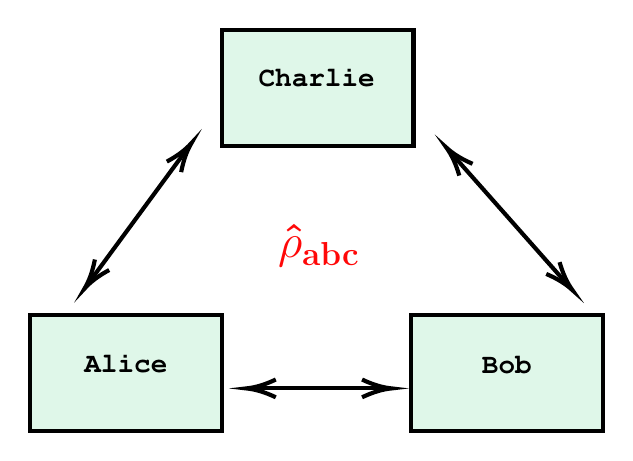
\begin{tikzpicture}[x=0.75pt,y=0.75pt,yscale=-1,xscale=1]
%uncomment if require: \path (0,300); %set diagram left start at 0, and has height of 300

%Shape: Rectangle [id:dp8194440686845581] 
\draw  [fill={rgb, 255:red, 223; green, 247; blue, 233 }  ,fill opacity=1 ][line width=1.5]  (177,190.34) -- (269.44,190.34) -- (269.44,246.4) -- (177,246.4) -- cycle ;
%Shape: Rectangle [id:dp04310487861766332] 
\draw  [color={rgb, 255:red, 0; green, 0; blue, 0 }  ,draw opacity=1 ][fill={rgb, 255:red, 223; green, 247; blue, 233 }  ,fill opacity=1 ][line width=1.5]  (269.44,53) -- (361.88,53) -- (361.88,109.06) -- (269.44,109.06) -- cycle ;
%Shape: Rectangle [id:dp32975298478620196] 
\draw  [fill={rgb, 255:red, 223; green, 247; blue, 233 }  ,fill opacity=1 ][line width=1.5]  (360.56,190.34) -- (453,190.34) -- (453,246.4) -- (360.56,246.4) -- cycle ;
%Straight Lines [id:da23895133806094215] 
\draw [line width=1.5]    (205.19,175.26) -- (253.14,110.03) ;
\draw [shift={(254.91,107.61)}, rotate = 126.32] [color={rgb, 255:red, 0; green, 0; blue, 0 }  ][line width=1.5]    (14.21,-4.28) .. controls (9.04,-1.82) and (4.3,-0.39) .. (0,0) .. controls (4.3,0.39) and (9.04,1.82) .. (14.21,4.28)   ;
\draw [shift={(203.41,177.68)}, rotate = 306.32] [color={rgb, 255:red, 0; green, 0; blue, 0 }  ][line width=1.5]    (14.21,-4.28) .. controls (9.04,-1.82) and (4.3,-0.39) .. (0,0) .. controls (4.3,0.39) and (9.04,1.82) .. (14.21,4.28)   ;
%Straight Lines [id:da6917940815863461] 
\draw [line width=1.5]    (379.71,112.03) -- (436.49,176.21) ;
\draw [shift={(438.47,178.45)}, rotate = 228.5] [color={rgb, 255:red, 0; green, 0; blue, 0 }  ][line width=1.5]    (14.21,-4.28) .. controls (9.04,-1.82) and (4.3,-0.39) .. (0,0) .. controls (4.3,0.39) and (9.04,1.82) .. (14.21,4.28)   ;
\draw [shift={(377.73,109.78)}, rotate = 48.5] [color={rgb, 255:red, 0; green, 0; blue, 0 }  ][line width=1.5]    (14.21,-4.28) .. controls (9.04,-1.82) and (4.3,-0.39) .. (0,0) .. controls (4.3,0.39) and (9.04,1.82) .. (14.21,4.28)   ;
%Straight Lines [id:da8377933043589034] 
\draw [line width=1.5]    (284.33,225.8) -- (348.32,225.8) ;
\draw [shift={(351.32,225.8)}, rotate = 180] [color={rgb, 255:red, 0; green, 0; blue, 0 }  ][line width=1.5]    (14.21,-4.28) .. controls (9.04,-1.82) and (4.3,-0.39) .. (0,0) .. controls (4.3,0.39) and (9.04,1.82) .. (14.21,4.28)   ;
\draw [shift={(281.33,225.8)}, rotate = 0] [color={rgb, 255:red, 0; green, 0; blue, 0 }  ][line width=1.5]    (14.21,-4.28) .. controls (9.04,-1.82) and (4.3,-0.39) .. (0,0) .. controls (4.3,0.39) and (9.04,1.82) .. (14.21,4.28)   ;

% Text Node
\draw (202.06,207.97) node [anchor=north west][inner sep=0.75pt]   [align=left] {{\fontfamily{pcr}\selectfont \textbf{Alice}}};
% Text Node
\draw (285.98,70.43) node [anchor=north west][inner sep=0.75pt]   [align=left] {\textbf{{\fontfamily{pcr}\selectfont Charlie}}};
% Text Node
\draw (393.58,208.77) node [anchor=north west][inner sep=0.75pt]   [align=left] {\textbf{{\fontfamily{pcr}\selectfont Bob}}};
% Text Node
\draw (316.39,157.15) node  [font=\LARGE,color={rgb, 255:red, 255; green, 8; blue, 8 }  ,opacity=1 ]  {$\mathlarger{\mathlarger{\mathlarger{\mathlarger{\mathbf{\hat{\rho }_{abc}}}}}}$};


\end{tikzpicture}

\caption{A qubit network, showing three parties, Alice, Bob and Charlie sharing an entangled state, represented by density operator $\hat{\rho}_{abc}$.}
\end{figure}
\noindent
For successfully performing a protocol between two parties, entanglement must exist between the qubits possessed by the two parties. The above diagram shows three parties Alice, Bob and Charlie, each possessing a qubit and their combined state is described by the density operator $\hat{\rho}_{abc}$. Then, suppose Alice and Bob want to perform a protocol while Charlie does not want to participate. In this case, a general operator for the system will be of the form:\\[0.2cm]
$$\hat{\mathrm{O}} = \sum\limits_i (\mathrm{\hat{M}_{i,ab}\otimes\hat{\mathds{1}_c}})\hat{\rho}_{abc}(\mathrm{\hat{M}^{\dagger}_{i,ab}\otimes\hat{\mathds{1}_c}})$$ where $\hat{M}_{i,ab}$ is some operator acting on the combined Hilbert space of Alice and Bob and the index $i$ runs over all the possible outcomes. Note that the operator does not interfere with Charlie's qubit. The probability of the $i^{\mathrm{th}}$ outcome is given by:
$$p_i = \Tr_{abc}[(\mathrm{\hat{M}^{\dagger}_{i,ab}\otimes\hat{\mathds{1}}_c})(\mathrm{\hat{M}_{i,ab}\otimes\hat{\mathds{1}}_c})\hat{\rho}_{abc}]\quad\xrightarrow[\text{system $c$}]{\text{Tracing out}} \Tr_{ab}[\mathrm{\hat{M}^{\dagger}_{i,ab}}\mathrm{\hat{M}_{i,ab}}\hat{\rho}_{ab}]$$
In this case, knowledge of Charlie's system is not neccessary for successfully applying the protocol by Alice and Bob. In the case Charlie decides to act on his qubit by some operator $\mathrm{\hat{N}_{i,c}}$, the total operator for the system will now be modified by:
$$\mathrm{\hat{M}_{i,ab}\otimes\hat{\mathds{1}_c}} \quad \longrightarrow \mathrm{\hat{M}_{i,ab}\otimes\hat{{N}}_{i,c}}$$
Now, for successfully performing the protocol, Alice and Bob must have a kmowledge of Charlie's operation since it could potentially affect the outcome of the protocol as the states are entangled. Thus, we have the following observations from the above discussion:
\begin{itemize}
    \item If the operator $\hat{\rho}_{ab}$ is separable, then the protocol cannot be performed successfully between Alice and Bob, as the two parties are not entangled. 
    \item If Charlie decides not to divulge any information about his system, the protocol cannot be applied as no correlation can be determined between the two parties Alice and Bob.
\end{itemize}
In this case, the above discussion on the knot theoretic approach to entangled quantum states can be of great use. As a demonstration, we consider building a three-qubit network such that: 
\begin{itemize}
    \item Bob and Charlie may never successfully perform any
    protocols without external help from Alice.
    \item Alice may
    have a chance to communicate with either Bob or Charlie
    if she wishes to.
\end{itemize}
The network is shown in the figure below:
\begin{figure}[H]
    \centering


\tikzset{every picture/.style={line width=0.75pt}} %set default line width to 0.75pt        

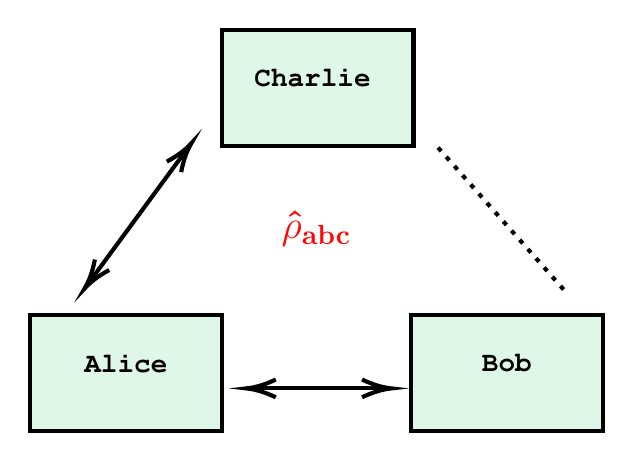
\begin{tikzpicture}[x=0.75pt,y=0.75pt,yscale=-1,xscale=1]
%uncomment if require: \path (0,300); %set diagram left start at 0, and has height of 300

%Shape: Rectangle [id:dp5199805559721411] 
\draw  [fill={rgb, 255:red, 223; green, 247; blue, 233 }  ,fill opacity=1 ][line width=1.5]  (197,162.92) -- (289.44,162.92) -- (289.44,218.97) -- (197,218.97) -- cycle ;
%Shape: Rectangle [id:dp4541164641811364] 
\draw  [color={rgb, 255:red, 0; green, 0; blue, 0 }  ,draw opacity=1 ][fill={rgb, 255:red, 223; green, 247; blue, 233 }  ,fill opacity=1 ][line width=1.5]  (289.44,25.57) -- (381.88,25.57) -- (381.88,81.63) -- (289.44,81.63) -- cycle ;
%Shape: Rectangle [id:dp04458970673752716] 
\draw  [fill={rgb, 255:red, 223; green, 247; blue, 233 }  ,fill opacity=1 ][line width=1.5]  (380.56,162.92) -- (473,162.92) -- (473,218.97) -- (380.56,218.97) -- cycle ;
%Straight Lines [id:da5905977694939716] 
\draw [line width=1.5]    (225.19,147.84) -- (273.14,82.6) ;
\draw [shift={(274.91,80.18)}, rotate = 126.32] [color={rgb, 255:red, 0; green, 0; blue, 0 }  ][line width=1.5]    (14.21,-4.28) .. controls (9.04,-1.82) and (4.3,-0.39) .. (0,0) .. controls (4.3,0.39) and (9.04,1.82) .. (14.21,4.28)   ;
\draw [shift={(223.41,150.26)}, rotate = 306.32] [color={rgb, 255:red, 0; green, 0; blue, 0 }  ][line width=1.5]    (14.21,-4.28) .. controls (9.04,-1.82) and (4.3,-0.39) .. (0,0) .. controls (4.3,0.39) and (9.04,1.82) .. (14.21,4.28)   ;
%Straight Lines [id:da10833960790906139] 
\draw [line width=1.5]  [dash pattern={on 1.69pt off 2.76pt}]  (393.73,82.36) -- (454.47,151.03) ;
%Straight Lines [id:da635570582048944] 
\draw [line width=1.5]    (304.33,198.37) -- (368.32,198.37) ;
\draw [shift={(371.32,198.37)}, rotate = 180] [color={rgb, 255:red, 0; green, 0; blue, 0 }  ][line width=1.5]    (14.21,-4.28) .. controls (9.04,-1.82) and (4.3,-0.39) .. (0,0) .. controls (4.3,0.39) and (9.04,1.82) .. (14.21,4.28)   ;
\draw [shift={(301.33,198.37)}, rotate = 0] [color={rgb, 255:red, 0; green, 0; blue, 0 }  ][line width=1.5]    (14.21,-4.28) .. controls (9.04,-1.82) and (4.3,-0.39) .. (0,0) .. controls (4.3,0.39) and (9.04,1.82) .. (14.21,4.28)   ;

% Text Node
\draw (222.06,180.54) node [anchor=north west][inner sep=0.75pt]   [align=left] {{\fontfamily{pcr}\selectfont \textbf{Alice}}};
% Text Node
\draw (303.98,43) node [anchor=north west][inner sep=0.75pt]   [align=left] {\textbf{{\fontfamily{pcr}\selectfont Charlie}}};
% Text Node
\draw (413.58,180.34) node [anchor=north west][inner sep=0.75pt]   [align=left] {\textbf{{\fontfamily{pcr}\selectfont Bob}}};
% Text Node
\draw (317.14,111.48) node [anchor=north west][inner sep=0.75pt]  [font=\Large,color={rgb, 255:red, 255; green, 8; blue, 8 }  ,opacity=1 ]  {$\mathlarger{\mathlarger{\mathlarger{\mathlarger{\mathbf{\hat{\rho }_{abc}}}}}}$};


\end{tikzpicture}

\caption{A qubit network, showing three parties, Alice, Bob and Charlie sharing an entangled state, represented by density operator $\hat{\rho}_{abc}$. The dotted line represent no connection between the two parties.}
\end{figure}
\noindent
The network can be easily described using the link polynomial language as: $\mathrm{P(a,b,c)= ac+ab}$ and thus we can immediately find a state that satisfies the above condition. The situation becomes more helpful when we consider higher number of qubits. Let us consider a four qubit network, where Alice, Bob, Charlie and Diana are the parties such that only the following parties can communicate:
\begin{itemize}
    \item Alice, Bob, and Charlie
    \item Alice, Bob, and Diana
    \item Alice and Charlie
\end{itemize}
\begin{figure}[H]
    \centering


\tikzset{every picture/.style={line width=0.75pt}} %set default line width to 0.75pt        

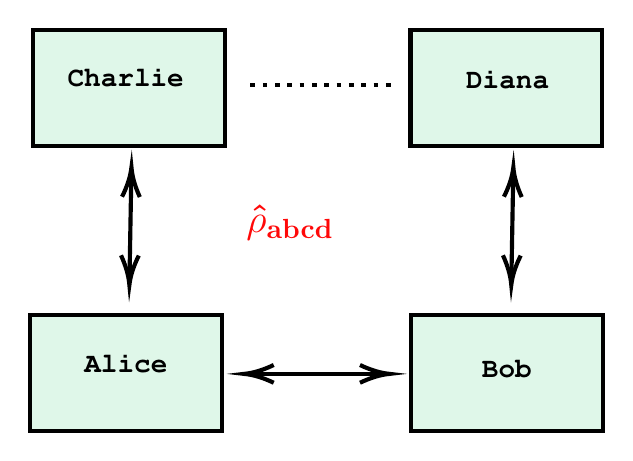
\begin{tikzpicture}[x=0.75pt,y=0.75pt,yscale=-1,xscale=1]
%uncomment if require: \path (0,300); %set diagram left start at 0, and has height of 300

%Shape: Rectangle [id:dp10277356992512154] 
\draw  [fill={rgb, 255:red, 223; green, 247; blue, 233 }  ,fill opacity=1 ][line width=1.5]  (197,162.92) -- (289.44,162.92) -- (289.44,218.97) -- (197,218.97) -- cycle ;
%Shape: Rectangle [id:dp015384298355835657] 
\draw  [color={rgb, 255:red, 0; green, 0; blue, 0 }  ,draw opacity=1 ][fill={rgb, 255:red, 223; green, 247; blue, 233 }  ,fill opacity=1 ][line width=1.5]  (198.44,25.57) -- (290.88,25.57) -- (290.88,81.63) -- (198.44,81.63) -- cycle ;
%Shape: Rectangle [id:dp7204404417404228] 
\draw  [fill={rgb, 255:red, 223; green, 247; blue, 233 }  ,fill opacity=1 ][line width=1.5]  (380.56,162.92) -- (473,162.92) -- (473,218.97) -- (380.56,218.97) -- cycle ;
%Shape: Rectangle [id:dp17140074186825027] 
\draw  [color={rgb, 255:red, 0; green, 0; blue, 0 }  ,draw opacity=1 ][fill={rgb, 255:red, 223; green, 247; blue, 233 }  ,fill opacity=1 ][line width=1.5]  (380.44,25.57) -- (472.88,25.57) -- (472.88,81.63) -- (380.44,81.63) -- cycle ;
%Straight Lines [id:da032463145441033014] 
\draw [line width=1.5]    (303.33,191.37) -- (367.32,191.37) ;
\draw [shift={(370.32,191.37)}, rotate = 180] [color={rgb, 255:red, 0; green, 0; blue, 0 }  ][line width=1.5]    (14.21,-4.28) .. controls (9.04,-1.82) and (4.3,-0.39) .. (0,0) .. controls (4.3,0.39) and (9.04,1.82) .. (14.21,4.28)   ;
\draw [shift={(300.33,191.37)}, rotate = 0] [color={rgb, 255:red, 0; green, 0; blue, 0 }  ][line width=1.5]    (14.21,-4.28) .. controls (9.04,-1.82) and (4.3,-0.39) .. (0,0) .. controls (4.3,0.39) and (9.04,1.82) .. (14.21,4.28)   ;
%Straight Lines [id:da7055775840806392] 
\draw [line width=1.5]    (245.05,145.52) -- (245.95,94.88) ;
\draw [shift={(246,91.88)}, rotate = 91.01] [color={rgb, 255:red, 0; green, 0; blue, 0 }  ][line width=1.5]    (14.21,-4.28) .. controls (9.04,-1.82) and (4.3,-0.39) .. (0,0) .. controls (4.3,0.39) and (9.04,1.82) .. (14.21,4.28)   ;
\draw [shift={(245,148.52)}, rotate = 271.01] [color={rgb, 255:red, 0; green, 0; blue, 0 }  ][line width=1.5]    (14.21,-4.28) .. controls (9.04,-1.82) and (4.3,-0.39) .. (0,0) .. controls (4.3,0.39) and (9.04,1.82) .. (14.21,4.28)   ;
%Straight Lines [id:da39607289649694266] 
\draw [color={rgb, 255:red, 0; green, 0; blue, 0 }  ,draw opacity=1 ][fill={rgb, 255:red, 44; green, 28; blue, 255 }  ,fill opacity=1 ][line width=1.5]    (429.05,145.52) -- (429.95,94.88) ;
\draw [shift={(430,91.88)}, rotate = 91.01] [color={rgb, 255:red, 0; green, 0; blue, 0 }  ,draw opacity=1 ][line width=1.5]    (14.21,-4.28) .. controls (9.04,-1.82) and (4.3,-0.39) .. (0,0) .. controls (4.3,0.39) and (9.04,1.82) .. (14.21,4.28)   ;
\draw [shift={(429,148.52)}, rotate = 271.01] [color={rgb, 255:red, 0; green, 0; blue, 0 }  ,draw opacity=1 ][line width=1.5]    (14.21,-4.28) .. controls (9.04,-1.82) and (4.3,-0.39) .. (0,0) .. controls (4.3,0.39) and (9.04,1.82) .. (14.21,4.28)   ;
%Straight Lines [id:da6546093054475423] 
\draw [line width=1.5]  [dash pattern={on 1.69pt off 2.76pt}]  (303.33,52.37) -- (332,52.37) -- (373.32,52.37) ;

% Text Node
\draw (222.06,180.54) node [anchor=north west][inner sep=0.75pt]   [align=left] {{\fontfamily{pcr}\selectfont \textbf{Alice}}};
% Text Node
\draw (213.98,43) node [anchor=north west][inner sep=0.75pt]   [align=left] {\textbf{{\fontfamily{pcr}\selectfont Charlie}}};
% Text Node
\draw (413.58,183.34) node [anchor=north west][inner sep=0.75pt]   [align=left] {\textbf{{\fontfamily{pcr}\selectfont Bob}}};
% Text Node
\draw (300.14,108.48) node [anchor=north west][inner sep=0.75pt]  [font=\Large,color={rgb, 255:red, 255; green, 8; blue, 8 }  ,opacity=1 ]  {$\mathlarger{\mathlarger{\mathlarger{\mathlarger{\mathbf{\hat{\rho }_{abcd}}}}}}$};
% Text Node
\draw (405.98,44) node [anchor=north west][inner sep=0.75pt]   [align=left] {\textbf{{\fontfamily{pcr}\selectfont Diana}}};


\end{tikzpicture}

\caption{The four qubit network, showing four parties, Alice, Bob, Charlie and Diana sharing an entangled state, represented by density operator $\hat{\rho}_{abcd}$. The dotted line represent no connection between the two parties.}
\end{figure}
We can easily see that the polynomial describing this network is $\mathrm{P(a,b,c,d) = abc+abd+ac}$. Thus a state can immediately be obtained using the algorithm described previously.
\section{Discussion and Conclusion}
\section{Acknowledgements}
\newpage
\section*{Appendix A: {\huge Quantum Information Basics}}
\addcontentsline{toc}{section}{Appendix A: Quantum Information Basics} % Optional
\subsection{Density Matrix}
\subsection{Peres-Horodecki Criterion}
\newpage


\section*{Appendix C: {\huge Code for Numeric Calculations}}
We used the \texttt{QuantumInformation.jl} package in \texttt{Julia} to perform the numerical calculations. The code provided below shows some basic calculations that we had used in this report. 
\addcontentsline{toc}{section}{Appendix C: { Code for Numerical Calculations}}
\begin{lstlisting}[language=Julia,label={lst:transmission}]
using QuantumInformation, LinearAlgebra, Latexify 
#example of a 3 qubit system: 3^2 link class mixed class

function ghz_n(n::Int64)
    up_f=zeros(2^n)
    a=up
    b=down
    for i =2:n 
        a=kron(a,up)
        b=kron(b,down)
    end
    return real.((a+b)/sqrt(2))
end
up = ket(1,2)
down = ket(2,2)

#defining the mixed state 
psi_3_2 = kron(ghz_n(3), ket(1,2))+kron(ghz_n(2), ket(1,2), ket(2,2));

#calculating the density matrix after tracing out the last qubit
rho_3_2 = round.(real.((ptrace(psi_3_2*psi_3_2', [2,2,2,2], 4))), digits=3) 
rho_3_2 = rho_3_2 ./tr(rho_3_2);

#calculating the partial transpose of the entire system
ppt_rho_3_2 = []
for i=1:3
    push!(ppt_rho_3_2, ptranspose(rho_3_2, [2,2,2], i));
end

#calculating the reduced traces 
red_rho_3_2 = []
for i= 1:3
    push!(red_rho_3_2, ptrace(rho_3_2, [2,2,2], i))
end

#calculating the eigenvalues of the PPT matrices
for i = 1:3
    println(round.(eigvals((ppt_rho_3_2[i])), digits=3))
end

#calculating the PPT matrices and their eigenvalues of the reduced system
for i = 1:3
    for j=1:2
    latexify(ptranspose(red_rho_3_2[i], [2,2], j))|>print
    end
end
for i = 1:3
    for j=1:1
    (round.(eigvals(ptranspose(red_rho_3_2[i], [2,2], j)), digits=3))|>println
    end
end
\end{lstlisting}
\bibliographystyle{plain}
\newpage
\bibliography{ref}
\end{document}
% References 
